% ignore chktex warning about dashes (no 8):
% chktex-file 8
% chktex-file 11
\documentclass[
final,
11pt,
a4paper,
DIV=11,
headinclude=true,
footinclude=false,
bibliography=totoc,
%two sides
twoside=true,  %true, false, semi
BCOR=5mm
]{scrbook}

\usepackage{../tex/preamble}

% Cover paper
\usepackage{pdfpages}

\usepackage{etoolbox}
\newtoggle{draftVersion}
%\toggletrue{draftVersion}
\togglefalse{draftVersion}

\begin{document}

\frontmatter

\includepdf{cover/cover.pdf}

\cleardoubleemptypage

%%% BEGIN ABSTRACTS %%%

\thispagestyle{plain}
\begin{otherlanguage}{portuguese}
{\fontfamily{lmr}\fontseries{b}\fontshape{n}\large\selectfont%
\begin{center}Resumo\end{center}}

Observações realizadas nas últimas três décadas confirmaram que 
o universo se encontra em um estado de expansão acelerada. Essa 
ace\-le\-ração é atribuída à presença da chamada energia escura, 
cuja origem permanece desconhecida. A maneira mais simples de se 
modelar a energia escura consiste em introduzir uma constante 
cosmológica positiva nas equações de Einstein, cuja solução no 
vácuo é então dada pelo espaço de de Sitter. Isso, por sua vez, 
indica que a cinemática subjacente ao espaço-tempo deve ser 
aproximadamente governada pelo grupo de de Sitter $SO(1,4)$, 
e não pelo grupo de Poincaré $ISO(1,3)$.

Nesta tese, adotamos tal argumento como base para a conjectura de 
que o grupo que governa a cinemática local é o grupo de de 
Sitter, com o desvio em relação ao grupo de Poincaré dependendo 
ponto-a-ponto do valor de um termo cosmológico variável. Com 
o propósito de desenvolver tal formalismo, estudamos a geometria 
de Cartan na qual o espaço modelo de Klein é, em cada ponto, um 
espaço de de Sitter com o conjunto de pseudo-raios definindo uma 
função não-constante do espaço-tempo.  Encontramos que o tensor 
de torção nessa geo\-metria adquire uma contribuição que não está 
presente no caso de uma constante cosmológica.  Fazendo uso da 
teoria das realizações não-lineares, estendemos a classe de 
simetrias do grupo de Lorentz $SO(1,3)$ para o grupo de de 
Sitter. Em seguida, verificamos que a estrutura da gravitação 
telepa\-ra\-lela--- uma teoria gravitacional equivalente 
à relatividade geral--- é uma geometria de Riemann-Cartan não 
linear.

Inspirados nesse resultado, construímos uma generalização da 
gravitação teleparalela sobre uma geometria de de Sitter--Cartan 
com um termo cosmológico dado por uma função do espaço-tempo, 
a qual é consistente com uma cinemática localmente governada pelo 
grupo de de Sitter. A função cosmológica possui sua própria 
dinâmica e emerge naturalmente acoplada não-minimalmente ao campo 
gravitacional, analogamente ao que ocorre nos modelos 
telaparalelos de energia escura ou em teorias de gravitação 
escalares-tensoriais. Característica peculiar do modelo aqui 
desenvolvido, a função cosmológica fornece uma contribuição para 
o desvio geodésico de partículas adjacentes em queda livre.  
Embora tendo sua própria dinâmica, a energia escura manifesta-se 
como um efeito da cinemática local do espaço-tempo.

\end{otherlanguage}


\cleardoubleemptypage

\thispagestyle{plain}
{\fontfamily{lmr}\fontseries{b}\fontshape{n}\large\selectfont%
\begin{center}Abstract\end{center}}

Observations during the last three decades have confirmed that
the universe momentarily expands at an accelerated rate, which is 
assumed to be driven by dark energy whose origin remains unknown.  
The minimal manner of modelling dark energy is to include 
a positive cosmological constant in Einstein's equations, whose 
solution in vacuum is de Sitter space. This indicates that the 
large-scale kinematics of spacetime is approximated by the de 
Sitter group $SO(1,4)$ rather than the Poincar\'e 
group~$ISO(1,3)$. 

In this thesis we take this consideration to heart and conjecture 
that the group governing the local kinematics of physics is the 
de Sitter group, so that the amount to which it is a deformation 
of the Poincar\'e group depends pointwise on the value of 
a nonconstant cosmological function. With the objective of 
constructing such a framework we study the Cartan geometry in 
which the model Klein space is at each point a de Sitter space 
for which the combined set of pseudoradii forms a nonconstant 
function on spacetime. We find that the torsion receives 
a contribution that is not present for a cosmological constant. 
Invoking the theory of nonlinear realizations we extend the class 
of symmetries from the Lorentz group $SO(1,3)$ to the enclosing 
de Sitter group. Subsequently, we find that the geometric 
structure of teleparallel gravity--- a description for the 
gravitational interaction physically equivalent to general 
relativity--- is a nonlinear Riemann--Cartan geometry.

This finally inspires us to build on top of a de Sitter--Cartan 
geometry with a cosmological function a generalization of 
teleparallel gravity that is consistent with a kinematics locally 
regulated by the de Sitter group. The cosmological function is 
given its own dynamics and naturally emerges nonminimally coupled 
to the gravitational field in a manner akin to teleparallel dark 
energy models or scalar-tensor theories in general relativity.  
New in the theory here presented, the cosmological function gives 
rise to a kinematic contribution in the deviation equation for 
the world lines of adjacent free-falling particles. While having 
its own dynamics, dark energy manifests itself in the local 
kinematics of spacetime.

\vspace{2\baselineskip}
\noindent
\textbf{Keywords:} dark energy, de Sitter special relativity, 
teleparallel gravity, cosmological function, Cartan geometry.

\vspace{\baselineskip}
\noindent
\textbf{Subjects:} gravitation, cosmology, special relativity.


%%% END ABSTRACTS %%%

\tableofcontents

\addchap{Acknowledgments}
\thispagestyle{empty}

This thesis has found its way into existence because of the 
dedication and kind-heartedness of various persons to whom 
I would like to express my gratitude.

In the first place I would like to thank Prof.~José Geraldo 
Pereira for having granted me the pleasure to collaborate under 
his guidance on truly interesting questions. The confidence he 
showed by giving me the space to come up with solutions, together 
with the advice he gave when these were hard to find, I hold in 
high esteem.

Further I would like to mention gratefully some of the present 
and past members of our research group; Lucas Lolli Savi for 
having introduced me, and Martin Kr\v{s}\v{s}ak, Adriana Araujo 
and Almeira del Carmen Sampson for interesting discussions.

I am indebted to CAPES for monetary support during four years of 
studying. Although it may be beyond their consent I would like to 
thank the Brazilian population for having financed this research, 
and for their hospitality in receiving me in their beautiful 
country. Unfortunately, I cannot assure the taxpayers that they 
will get value for money.

Exchanging \emph{het Pajottenland} for a concrete jungle not 
always has been straightforward. It is with the greatest 
admiration that I thank Fernanda for her continuous support, 
patience, and companion along the road we are exploring.

Last but foremost I thank my family for their unconditional and 
warm understanding of the choices I make. It is their love and 
unabating support which inspire me to carve out this path so far 
away from home.

\cleardoubleemptypage
\thispagestyle{empty}

\vspace*{2cm}
%\vspace*{\fill}

\begin{center}
\begin{minipage}{12cm}
  \textit{%
    And different forms of \ldots~make laws in different ways.  
    Some operate democratically; in others the aristocrats rule; 
    and in still others a single tyrant makes the laws. It all 
    depends on their various interests. They all claim that what 
    is advantageous to themselves is justice for the people they 
    rule. Anyone who violates this principle they punish as 
    a lawbreaker, and they brand that person as unjust. That is 
    what I mean, sir, when I say that there exists in all states 
    the same principle of justice, and that is the interest of 
    the established \ldots. In all cases the \ldots~has the 
    power, so the only reasonable conclusion is that everywhere 
    there is but one principle of justice: the interest of the 
    stronger.
  }

\blankline
\hfill
Thrasymachos in Republic I, 338d-339a, Plato

\hfill
{\small(Translation by B.~Jowett)}
\end{minipage}
\end{center}

\mainmatter%

\chapter{Prolegomena}

The gravitational force was the first of the four fundamental 
interactions in physics to have been given a quantitative 
description when Sir Isaac Newton stated his law of universal 
gravitation in 1687. Well over three centuries later the 
ubiquitous gravitational interaction still lacks a solid 
understanding both at the smallest of unobservable and the 
largest of observable length scales, considering that Einstein's 
general relativity remains in full control in between.  At very 
small distances and high energies, i.e., around the Planck energy 
density, a quantization of the gravitational interaction is 
expected indispensable~\cite{Padmanabhan:1987au, Kiefer:2007ria}.  
The problem of constructing quantum gravity is thus of direct 
relevance to understand the physics of the interior of black 
holes and the stages of the universe closely following the big 
bang, but trying to solve it head-on might result too ambitious.

It is not impossible that general relativity comes short in 
describing the evolution of the large-scale structure of the 
universe, so that it may not be the complete story at the 
classical level already. Until the nineties of the last century 
the gravitational force had been observed to be attractive only, 
such that the expansion of the universe was believed to be 
decelerating. In 1998, however, comparison of the apparent 
luminosity and redshift for a set of Type Ia supernovae showed 
for the first time that the expansion of the universe fairly 
recently started to accelerate~\cite{Perlmutter:1998np, 
  Riess:1998cb}, i.e., gravity has a repulsive component.  
According to Einstein's equations such a component can only be 
the result of some sort of energy whose pressure to density ratio 
is less than $-1/3$, coined \emph{dark energy} due to this exotic 
equation of state.  The simplest candidate for dark energy is the 
cosmological constant $\Lambda$, which has a pressure to density 
ratio equal to $-1$ if interpreted as a perfect fluid.  
Observations indicate it accounts for about 70\% of the total 
energy density, whereas the remaining 30\% is almost completely 
made up of pressureless dust~\cite{Ade:2015xua}. It is part of 
the standard model of cosmology--- the so-called $\Lambda$ cold 
dark matter ($\Lambda$CDM) model--- that dark energy is the 
cosmological constant, being the simplest model consistent with 
the present state of observational data.  Nevertheless, the 
absolute constancy of the cosmological constant due to its 
inability to interact with other forms of energy, as well as the 
lack of a physical explanation for its observed value which is 
close to $10^{-52}\:\mrm{m}^{-2}$, give it a somewhat artificial 
appearance unless one is willing to interpret it as another 
fundamental constant of nature.  Alternative models for the 
cosmological constant to explain the observed dark energy come in 
a number of varieties. Some of these models minimally couple 
exotic scalar fields to general relativity, while others modify 
gravity directly~\cite{Copeland:2006wr}.  Generally they account 
for some form of dark energy with a dynamical equation of state 
that mimics a present-day cosmological constant driving the 
accelerated expansion of the universe.

The existence of dark energy suggests that the large-scale 
geometry of spacetime must be considered a deformation of de 
Sitter instead of Minkowski space, for it is the former that 
solves Einstein's equations in the absence of further 
contributions to the energy-momentum density. The kinematics of 
physics at this scale is consequently expected to be governed by 
the de Sitter group $SO(1,4)$ in place of the Poincar\'e group 
$ISO(1,3)$, for what reason its characterization by special 
relativity is to be replaced with the more general de Sitter 
special relativity~\cite{Aldrovandi:2006vr}. The degree to which 
the kinematic group is deformed from the Poincar\'e to the de 
Sitter group depends on the value of $\Lambda$, which in the case 
of dynamical dark energy must be allowed to become time 
dependent. In addition, there seems no reason to suppose \emph{a 
  priori} that dark energy should remain homogeneous over scales 
where the cosmological principle breaks down, such that $\Lambda$ 
and the corresponding kinematic group become spacetime dependent 
in principle. According to this scheme, different regions in 
spacetime are approximated by de Sitter spaces with different 
cosmological constants whose values are given by the cosmological 
function $\Lambda$. Because the cosmological function modifies 
the local kinematics of physics one anticipates it to form an 
integral part of the geometry of spacetime.

The working objective of this thesis consists in finding the 
precise mathematical structure to implement this scheme and to 
apply it in order to construct a generalization of the 
gravitational interaction coupled to the cosmological function.  
The set of mathematical tools that are necessary to describe the 
spacetimes we are after is contained in Cartan geometry, which is 
a nonhomogeneous version of Klein 
geometry~\cite{sharpe1997diff_geo}. Klein geometries describe 
homogeneous spaces in terms of their Lie symmetry groups, which 
connect any two of the spaces' points.  When these symmetries are 
retained only between points that are separated by an 
infinitesimal element, Cartan geometry introduces inhomogeneities 
that are quantified by nonzero values for the curvature or 
torsion two-forms or both. Accordingly, the space characterized 
by the Cartan geometry is at each point approximated by the 
corresponding homogeneous Klein space. It becomes intuitively 
clear that we need to consider a Cartan geometry modeled on de 
Sitter space in order to achieve our purpose, but with the 
peculiarity that the set of cosmological constants, i.e., the 
cosmological function, is nonconstant on spacetime.

It appears sensible to have the cosmological function implemented 
in this manner as the obtained geometry reduces to 
a Riemann--Cartan geometry when $\Lambda$ vanishes everywhere.  
This is nothing but a Cartan geometry modeled on Minkowski space, 
from which it is well known that its zero-torsion variant is the 
framework that underlies general relativity. When it is curvature 
instead of torsion that is turned off, the resulting 
Riemann--Cartan geometry is used to describe teleparallel 
gravity. This theory is physically equivalent to general 
relativity in its description of the gravitational interaction, 
although conceptually it is rather unlike 
it~\cite{aldrovandi:2012tele}.  A key difference between the two 
alternatives is that the spin connection of teleparallel gravity 
accounts for inertial effects only, such that it does not bear 
any gravitational degrees of freedom. Inertial and gravitational 
effects are therefore logically separated, which makes the 
description robust against a hypothetical breakdown of the weak 
equivalence principle. When aiming for a generalization of the 
gravitational interaction in the presence of the cosmological 
function, we shall take as our starting point the description of 
teleparallel gravity rather than the one of general relativity.  
This way gravitational degrees of freedom are encoded in the 
torsion of the geometry, while the spin connection represents 
inertial effects due to the noninertiality of the frame and 
kinematic effects due to the cosmological function. 

To conclude this introductory chapter we give a brief outline of 
the thesis.
\begin{itemize}
  \item[$\circ$] Basic tools regarding differentiable manifolds, 
    Lie groups and principal fibre bundles are recalled 
    in~\S\ref{ch:prelim}, which are preliminary to a modern 
    treatment of geometry.%
    \vspace{3pt}
  \item[$\circ$] Geometry is the central theme 
    of~\S\ref{ch:Cartan_geo}. The abstract geometries of 
    Ehresmann connections are introduced first, after which the 
    Lie theoretic descriptions of homogeneous Klein geometries 
    and nonhomogeneous Cartan geometries are looked at in detail.  
    We additionally revise the relation between Ehresmann and 
    Cartan connections.
    \vspace{3pt}
  \item[$\circ$] \S\ref{ch:dSC_geometry}, based on 
    Ref.~\cite{Jennen:2014mba}, constructs de Sitter--Cartan 
    geometry, which is a Cartan geometry modeled on de Sitter 
    space so that the cosmological function is nonconstant.  
    Afterwards, a nonlinear realization of the Cartan geometry is 
    considered to render the construction $SO(1,4)$ invariant.%
    \vspace{3pt}
  \item[$\circ$] In~\S\ref{ch:review_TG} we review teleparallel 
    gravity and clarify how its historical interpretation as 
    a gauge theory for the Poincar\'e translations can be 
    understood in terms of a nonlinear Riemann--Cartan geometry.
    \vspace{3pt}
  \item[$\circ$] \S\ref{ch:dSTG}, based on 
    Ref.~\cite{Jennen:2015bxa}, introduces de Sitter teleparallel 
    gravity, which generalizes teleparallel gravity for the 
    cosmological function using de Sitter--Cartan geometry. It is 
    shown what the phenomenology is of the kinematic effects due 
    to a nonvanishing cosmological function. Finally, we 
    postulate the dynamics of the gravitational field coupled to 
    the cosmological function.
    \vspace{3pt}
  \item[$\circ$] The thesis is concluded 
    in~\S\ref{ch:conclusions}.
\end{itemize}

\chapter{Preliminaries}
\label{ch:prelim}

In this first of three mathematically inclined chapters we 
provide a selective survey of differentiable manifolds and Lie 
groups preliminarily to the study of Cartan geometry in the 
following chapter. This review is mainly based on the first 
chapter of the beautiful exposition~\cite{kob1996found} and the 
book~\cite{nakahara:2003gt}.

\section{Differentiable manifolds}

\subsection{Topological spaces and differentiable atlases}

\begin{definition}
Let $\mc{S}$ be a set and let $\mc{P}(\mc{S}) = \{ S \mid 
S \subseteq \mc{S} \}$ be the power set of $\mc{S}$, i.e., the 
collection of subsets of $\mc{S}$. A subset $\tau_\mc{S}$ of 
$\mc{P}(\mc{S})$ is a \emph{topology} on $\mc{S}$ if the 
following is true, namely,
\begin{itemize}
  \item[(i)] The empty set $\emptyset$ and $\mc{S}$ itself are in 
    $\tau_\mc{S}$;
  \item[(ii)] The union of any number of elements of 
    $\tau_\mc{S}$ is an element of $\tau_\mc{S}$;
  \item[(iii)] The intersection of any finite number of elements 
    of $\tau_\mc{S}$ is an element of $\tau_\mc{S}$.
\end{itemize}
The pair $(\mc{S},\tau_\mc{S})$ is called a topological space and 
the subsets of $\mc{S}$ that are in the topology are referred to 
as \emph{open sets}. The elements of $\mc{S}$ are called 
\emph{points}. We shall generally abbreviate notation and denote 
the topological space simply by $\mc{S}$.
\end{definition}

This at first sight rather abstract construction gives us a 
qualitative notion of closeness between points of a set. This 
notion is obtained when the topology is used to define 
convergence of sequences in a topological space.

\begin{definition}
A sequence of points $x_1, \ldots x_n, \ldots =
{\{x_n\}}_{n=1}^\infty$ \emph{converges} to the point $x$ if for 
any open set $U$ that contains $x$ there is a natural number 
$n_U$ such that the tail ${\{x_n\}}_{n > n_U}$ is in $U$. The 
convergence of the sequence is denoted by $x_n 
\overset{\tau_\mc{S}}{\longrightarrow} x$.
\end{definition}

The points ${\{x_n\}}_{n > n_U}$ are said to be closer to $x$ 
than $x_{n_U}$. If $V$ is an open subset of $U$, then 
${\{x_n\}}_{n > n_V}$ is a subtail of ${\{x_n\}}_{n > n_U}$ and 
$n_V \geq n_U$, so that the points in $V$ are closer to $x$ than 
the points in $U/V$. By considering a countable series of open 
subsets that contain $x$, the points of the corresponding 
subtails get arbitrarily close to $x$. To assure oneself that 
this abstraction is natural, it is useful to concretize it for 
the set $\mathds{R}^d$ of real $d$-tuples $x = (x^1,\ldots 
x^\mu,\ldots x^d)$.

\begin{example}
The \emph{usual topology} on $\mathds{R}^d$ is constructed as 
follows. For any point $x$ and any positive real number $r$, the 
\emph{open ball} with center $x$ and radius $r$ is defined by
\begin{equation*}
B(x,r) = \{y \in \mathds{R}^d \mid \|x-y\| < r \}.
\end{equation*}
The open sets $U$ that constitute the usual topology are those 
that for each $x \in U$ encompass an open ball with center $x$.  
Consider a convergent sequence $x_n \to x$ with respect to the 
usual topology. Let a collection of open sets that contain $x$ be 
given by $B(x,r)$ for any strictly positive $r$. Since the 
sequence $\{x_n\}$ converges to $x$, there is for any radius 
a number $n_r$ such that $B(x,r)$ contains the tail ${\{x_n\}}_{n 
  > n_r}$, that is, $\|x_n - x\| < r$ for any $n > n_r$. When $r$ 
gets arbitrary small, the elements of the sequence contained in 
$B(x,r)$ come arbitrarily close to $x$, generally denoted by 
$\lim_{n\to\infty}x_n = x$.
\end{example}

A subset $N$ of $\mc{S}$ is a \emph{neighborhood} of a point $x$ 
if $N$ encompasses an open set to which $x$ belongs. If $N$ is 
open it is called an \emph{open neighborhood}. Evidently, the 
elements of the usual topology on $\mathds{R}^d$ are open 
neighborhoods of any of its points.

A topological space $(\mc{S},\tau_\mc{S})$ is a \emph{Hausdorff 
  space} if for any two points there exist disjoint 
neighborhoods. The set $\mathds{R}^d$ with the usual topology is 
an example of a Hausdorff space. Indeed, for any two points $x_1$ 
and $x_2$ there exist $B(x_i,r)$ with $r \leq \|x_1-x_2\|/2$.

Let $\mc{S}$ and $\mc{T}$ be topological spaces. A function 
$\varphi : \mc{S} \to \mc{T}$ is \emph{continuous} if the 
preimage of any open subset of $\mc{T}$ is open in $\mc{S}$, 
i.e., $\varphi^{-1}(V) \in \tau_\mc{S}$ whenever $V \in 
\tau_\mc{T}$.  The function $\varphi$ is \emph{homeomorphic} if 
it is a bijection and both $\varphi$ and $\varphi^{-1}$ are 
continuous. This implies that open sets of $\mc{S}$ are mapped to 
open sets of $\mc{T}$.  When there exists a homeomorphism between 
two topological spaces they are said to be homeomorphic.  In 
particular, if a mapping $\varphi : \mc{S} \to \mathds{R}^d$ is a 
homeomorphism, $\mc{S}$ is homeomorphic to $\mathds{R}^d$.

Naturally, not every topological space is homeomorphic to 
$\mathds{R}^d$. We are nonetheless interested in topological 
spaces whose open sets are homeomorphic to the open sets in 
$\mathds{R}^d$. To provide a topological space with such a 
structure, we first define it.

\begin{definition}
A \emph{differentiable atlas} of dimension $d$ for a topological 
space $\mc{S}$ is a collection of pairs $\{(U_i,\varphi_i)\}$ for 
which the following is true:
\begin{itemize}
  \item[(i)] Every $U_i$ is an open set of $\mc{S}$ and $\cup_i 
    U_i = \mc{S}$;
  \item[(ii)] Each $\varphi_i$ is a homeomorphism from $U_i$ onto 
    an open subset of $\mathds{R}^d$;
  \item[(iii)] Whenever $U_i \cap U_j$ is nonempty the 
    homeomorphism $\varphi_j \circ \varphi_i^{-1} : \varphi_i(U_i 
    \cap U_j) \to \varphi_j(U_i \cap U_j)$ is differentiable, 
    i.e., of class $C^\infty$.
\end{itemize}
The pairs $(U_i,\varphi_i)$ are called \emph{coordinate charts} 
or just charts. The second item makes sense because the sets 
$U_i$ are topological subspaces of $\mc{S}$ with topologies
\begin{equation*}
  \tau_{U_i} = \{U_i \cap U \mid U \in \tau_\mc{S}\}.
\end{equation*}
When the last condition is dropped, the atlas is said to be 
topological instead of differentiable.
\end{definition}

\begin{definition}
A \emph{differentiable manifold} $\mc{M}$ of dimension $d$ is a 
Hausdorff space on which is defined a $d$-dimensional smooth 
atlas.
\end{definition}

The above defined manifold is for obvious reasons also called a 
\emph{real} differentiable manifold. A complex (analytic) 
$d$-dimensional manifold is readily constructed by demanding that 
the homeomorphisms $\varphi_i$ of the coordinate charts map onto 
open subsets of $\mathds{C}^d$. From now on, by a manifold we 
shall mean a real differentiable manifold.

The smoothness of the transition functions $\varphi_j \circ 
\varphi_i^{-1}$ can be written as follows in terms of coordinate 
charts. Consider a nonempty intersection $U_i \cap U_j$ on which 
there are defined two coordinate systems $x^\mu = \varphi_i$ and 
$y^\mu = \varphi_j$ taking values in some open set of 
$\mathds{R}^d$. The transition function on this open set takes 
the form $y^\mu(x^\nu) = \varphi_j \circ \varphi_i^{-1}(x^\nu)$.  
Differentiability of such a mapping means that the functions 
$y^\mu(x^\nu)$ are smooth, so that $\pd y^\mu/\pd x^\nu$ and 
higher order derivatives exist.

A mapping $f$ from a $d$-dimensional manifold $\mc{M}$ to a 
$d'$-dimensional manifold $\mc{M}'$ is differentiable if for 
every chart $(U_i,\varphi_i)$ of $\mc{M}$ and every chart 
$(V_j,\psi_j)$ of $\mc{M}'$ such that $f(U_i) \subset V_j$, the 
$\mathds{R}^{d'}$-valued function $\psi_j \circ f \circ 
\varphi_i^{-1} : \varphi_i(U_i) \to \psi_j(V_j)$ is 
differentiable. We shall denote the latter equally by $f$ or 
$f^{\mu'}$, where $\mu'=1,\ldots d'$. If we denote $x^\mu 
= \varphi_i$ and $y^{\mu'}=\psi_j$, the mapping may be expressed 
as $y^{\mu'} = f^{\mu'}(x^\mu)$. If $f$ is a bijection and its 
inverse is differentiable, it is called a \emph{diffeomorphism}.  
One may conclude that $d = d'$ because all the matrices $\psi_j 
\circ f \circ \varphi_i^{-1}$ are invertible as well. If the 
diffeomorphism goes from $\mc{M}$ to itself, it is also called 
a \emph{transformation}.

At this point it is appropriate to dedicate a few lines to the 
relationship between diffeomorphisms and coordinate 
transformations on a manifold $\mc{M}$, on which there are 
defined two atlases $\{(U_i,\varphi_i)\}$ and $\{(V_j,\psi_j)\}$.  
For any two overlapping charts $(U_i,\varphi_i)$ and 
$(V_j,\psi_j)$ a \emph{coordinate transformation} is defined by
\begin{equation*}
  \psi_j \circ \varphi_i^{-1} : \varphi_i(U_i \cap V_j) \to 
  \psi_j(U_i \cap V_j) : x^\mu \mapsto y^\mu(x^\nu) = \psi_j 
  \circ \varphi_i^{-1}(x^\nu).
\end{equation*}
From the definition of a differentiable atlas it follows that a 
coordinate transformation is a smooth invertible transformation 
on $\mathds{R}^d$. Concretely, the points of $\mc{M}$ with 
coordinates $x^\mu$ are given new coordinates $y^\mu$, but the 
points themselves have not changed.  On the other hand, given a 
diffeomorphism $f: \mc{M} \to \mc{M}$, we may consider its 
representation on $\mathds{R}^d$, namely,
\begin{equation*}
  \varphi_j \circ f \circ \varphi_i^{-1} : \varphi_i(U_i \cap 
  f^{-1}(U_j)) \to \varphi_j( f(U_i) \cap U_j): x^\mu \mapsto 
  y^\mu(x^\nu) = \varphi_j \circ f \circ \varphi_i^{-1}(x^\nu).
\end{equation*}
The point with coordinates $x^\mu$ is mapped to another point 
with coordinates $y^\mu$, whereas the coordinate atlas itself has 
been left untouched. Diffeomorphisms and coordinate 
transformations can be identified with each other on subdomains 
of $\mathds{R}^d$ by choosing $\psi_j = \varphi_j \circ f$ or $f 
= \varphi^{-1}_j \circ \psi_j$.  Whether one prefers to think 
about the transformation $x^\mu \mapsto y^\mu(x^\nu)$ as a 
coordinate transformation (the \emph{passive} point of view) or a 
diffeomorphism (the \emph{active} point of view) is not relevant 
mathematically.

\subsection{Tensor fields}

There are two subclasses of mappings on a given manifold $\mc{M}$ 
that are worthwhile to consider explicitly. The first consists of 
the \emph{curves} $x_t$, which map open intervals of $\mathds{R}$ 
into $\mc{M}$, i.e., $t \in (a,b) \mapsto x_t \in \mc{M}$. We 
shall assume that a curve does not intersect with itself, 
although they may form loops. A second important class of 
mappings are made up by the functions $f : \mc{M} \to 
\mathds{R}$, which assign a real number to each point of the 
manifold. The set of differentiable functions on $\mc{M}$ will be 
given the name $\mathscr{F}(\mc{M})$. With the help of a 
coordinate chart $(U_i,\varphi_i)$ one readily obtains a curve 
$\varphi_i \circ x_t$ in $\varphi_i(U_i) \subset \mathds{R}^d$ 
and a function $f \circ \varphi_i^{-1}$ on $\varphi_i(U_i)$. We 
generally shall write them as $x_t^\mu = \varphi_i(x_t)$ and 
$f(x^\mu) = f \circ \varphi_i^{-1}(x^\mu)$, respectively.

The \emph{tangent vector} $X$ to a curve $x_t$ at the point $x 
= x_{t_0}$ is the mapping $\mathscr{F}(x_{t_0}) \to \mathds{R}$ 
defined by
\begin{equation}
\label{eq:def_tangVec}
  X_x f = \frac{d}{dt}(f\circ x_t)|_{t_0},\quad
  \text{for any}~f\in\mathscr{F}(x_{t_0}),
\end{equation}
In terms of a local coordinate system $(U_i,\varphi_i)$, this is 
expressed as $\dot{x}_t^\mu\pd_\mu|_{t_0}f(x^\nu)$, where the dot 
means differentiation with respect to $t$. The tangent vector to 
$x_t$ at any point along the curve is therefore given by
\begin{equation}
\label{eq:tangVec_coor}
  X^\mu \frac{\pd}{\pd x^\mu} = \frac{dx_t^\mu}{dt} 
  \frac{\pd}{\pd x^\mu},
\end{equation}
which is the directional derivative along the curve. If 
$(V_j,\psi_j)$ is a second coordinate chart such that $x = 
x_{t_0} \in V_j$, one also may write~\eqref{eq:def_tangVec} as 
$\dot{y}_t^\mu\pd_\mu|_{t_0}f(y^\nu)$. It follows directly that 
the components of a tangent vector at $x$
transform according to
\begin{equation*}
  X^\mu \mapsto X^\nu \left.\frac{\pd y^\mu}{\pd 
      x^\nu}\right|_{x}
\end{equation*}
under the coordinate transformation $x^\mu \mapsto y^\mu(x^\nu) = 
\psi_j\circ\varphi_i^{-1}(x^\nu)$. 

Obviously, at any point $x$ the tangent vector is a linear 
operator on the space $\mathscr{F}(x)$, i.e., for any two 
functions $f$ and $g$ it is true that $X(f+g) = X(f) + X(g)$.  
Furthermore, it satisfies Leibniz's rule, i.e., $X(fg) = X(f)g + 
fX(g)$. Under the natural addition and scalar multiplication, the 
set of tangent vectors forms a vector space at any $x$, which is 
called the \emph{tangent space} $T_x \mc{M}$.  
From~\eqref{eq:tangVec_coor} it is evident that the collection 
$\{\pd/\pd x^\mu\}$ forms a basis for the tangent space, so that 
$\dim T_x\mc{M} = \dim \mc{M}$. For obvious reasons it is called 
a \emph{coordinate basis}.

A \emph{vector field} $X$ on $\mc{M}$ is obtained by smoothly 
assigning a tangent vector at any point in $\mc{M}$. More 
precisely, the function $Xf$, being defined pointwise by $(Xf)(x) 
= X_x f$, is differentiable whenever $f \in \mathscr{F}(\mc{M})$.  
Vector fields are thus mappings of $\mathscr{F}(\mc{M})$ onto 
itself, the set of which we shall denote by 
$\mathscr{X}(\mc{M})$. They constitute an infinite-dimensional 
vector space under the natural addition and scalar 
multiplication.  Moreover, it is a Lie algebra\footnote{See 
  \S\ref{sec:LieGrAlg} for the definition for a Lie algebra.} 
with the bracket given by $[X,Y]f = X(Yf)-Y(Xf)$, which on 
a local coordinate patch is expressed as ${[X,Y]}^\mu = X^\nu 
\pd_\nu Y^\mu - Y^\nu \pd_\nu X^\mu$. The bracket is 
a commutator, i.e., $[X,Y] = -[Y,X]$ and therefore satisfies the 
Jacobi identity
\begin{equation*}
  [[X,Y],Z] + [[Y,Z],X] + [[Z,X],Y] = 0.
\end{equation*}

If a collection $\{e_a\}$, with $a = 1,\ldots \dim\mc{M}$, of 
vector fields on $\mc{M}$ is at any point on which they are 
defined a basis for the tangent space, it is said to be 
a \emph{frame}.  The commutator of two elements of the frame can 
at any point be written as a linear combination of the frame 
fields, i.e.,
\begin{equation}
\label{eq:frame_manifold}
  [e_a,e_b] = c\ind{_{ab}^c}(p) e_c,
\end{equation}
where the nonconstant $c\ind{_{ab}^c}$ are called the 
\emph{structure functions} of the frame. Note that the structure 
functions of a coordinate basis vanish. When it is possible to 
define a frame on the whole of $\mc{M}$, the manifold is said to 
be \emph{parallelizable}.

The \emph{total differential} $df$ of a function $f$ is the 
$\mathscr{F}(\mc{M})$-linear functional on the set of vector 
fields $\mathscr{X}(\mc{M})$ that is defined pointwise by
\begin{equation}
\label{eq:totDeriv}
  df_x(X) = X_x(f),
  \quad\text{for any}~X\in\mathscr{X}(\mc{M}).
\end{equation}
In a local coordinate system $(U_i,\varphi_i)$ such that $x^\mu = 
\varphi_i$,~\eqref{eq:totDeriv} implies $dx^\mu(\pd_\nu) = 
\delta^\mu_\nu$.  Hence, the set $\{dx^\mu\}$ forms a dual set to 
the coordinate basis and spans the \emph{cotangent space} 
$T^\ast_p\mc{M}$, which is equal in dimension to $T_p\mc{M}$.  
Because $df(X) = X^\nu df(\pd_\nu) = X^\nu\pd_\nu f = X^\nu 
\pd_\mu f dx^\mu(\pd_\nu)$, it is obvious that $df = \pd_\mu f 
dx^\mu$.  Of course, not any element $\omega_\mu dx^\mu$ of the 
cotangent space can be written as a total differential of a 
function.  A \emph{one-form} $\omega : \mathscr{X}(\mc{M}) \to 
\mathscr{F}(\mc{M})$ is a smooth assignment of an element of the 
cotangent space at any point along $\mc{M}$ whereby it is meant 
that $\omega(X)$ is differentiable whenever $X$ is 
differentiable.  From now on the set of vector fields and the set 
of one-forms are denoted by $T\mc{M} = \mathscr{X}(\mc{M})$ and 
$T^\ast\mc{M}$, respectively.  We remark that in a local 
coordinate system one finds that $\omega(X) = \omega_\mu X^\mu$, 
from which it is readily concluded that a coordinate 
transformation $x^\mu \mapsto y^\mu(x^\nu)$ induces at any point 
a concomitant transformation on the components of the one-form 
according to $\omega_\mu \mapsto \omega_\nu \pd x^\nu / \pd 
y^\mu$.

It is then possible to interpret a vector field as a mapping of 
one-forms into functions by identifying $X(\omega) = \omega(X)$, 
which in a local coordinate system gives meaning to the equality 
$\pd_\mu dx^\nu = \delta^\nu_\mu$. Such an interpretation paves 
the way for the introduction of differentiable multilinear 
mappings
\begin{equation*}
  T : \underbrace{T^*\mc{M} \times \dots 
    T^*\mc{M}}_{r~\text{times}} \times \underbrace{T\mc{M} \times 
    \dots T\mc{M}}_{s~\text{times}} \to \mathscr{F}(\mc{M}),
\end{equation*}
which are named $(r,s)$-type tensor fields and whose collection 
we shall label by $T^r_s\mc{M}$. Elements of $T^r_0\mc{M}$ are 
also called \emph{contravariant} tensor fields, while those of 
$T^0_s\mc{M}$ go by the name of \emph{covariant} tensors. The 
\emph{tensor product} $\otimes$ of two tensor fields $T \in 
T^{r_1}_{s_1}\mc{M}$ and $S \in T^{r_2}_{s_2}\mc{M}$ is the 
$(r_1+r_2, s_1+s_2)$-type tensor field defined through
\begin{multline*}
  (T \otimes S)(\omega_1, \ldots \omega_{r_1}, \eta_1, \ldots 
  \eta_{r_2}, X_1, \dots X_{s_1}, Y_1, \dots Y_{s_2}) \\
  = T(\omega_1, \ldots \omega_{r_1}, X_1, \dots X_{s_1})
    S(\eta_1, \ldots \eta_{r_2}, Y_1, \dots Y_{s_2}),
\end{multline*}
for any set of one-forms $(\{\omega_i\},\{\eta_j\})$ and vector 
fields $(\{X_i\},\{Y_j\})$. A tensor field $T$ is expanded in 
some local coordinate system according to 
$T\ind{^{\mu_1\cdots\mu_r}_{\nu_1\cdots\nu_s}} \pd_{\mu_1} 
\otimes \cdots \pd_{\mu_r} \otimes dx^{\nu_1} \otimes \cdots 
dx^{\nu_s}$.

A mapping $f : \mc{M} \to \mc{N}$ between two manifolds induces a 
mapping $f^*: \mathscr{F}(\mc{N}) \to \mathscr{F}(\mc{M})$ 
between their sets of functions, defined by
\begin{equation*}
  (f^* g)(x) = g(f(x)),\quad\text{for any}~x\in\mc{M}.
\end{equation*}
Since the function $g$ on $\mc{N}$ is pulled back to a function 
$f^* g$ on $\mc{M}$, $f^*g$ is called the \emph{pullback} of $g$ 
by the mapping $f$. The \emph{pushforward} of a vector $X \in T_x 
\mc{M}$ is the vector $f_*X$ tangent to $\mc{N}$ at $f(x)$ such 
that
\begin{equation*}
  {(f_*X)}_{f(x)}(g) = X_x(f^*g),
  \quad\text{for any}~g \in \mathscr{F}(\mc{N}).
\end{equation*}
Consequently, the pullback $f^* : T^*\mc{N} \to T^*\mc{M}$ of a 
one-form is defined pointwise as
\begin{equation*}
  {(f^*\omega)}_x(X) = \omega_{f(x)}(f_*X),
  \quad\text{for any}~X\in T_x\mc{M}.
\end{equation*}
The pushforward and pullback are generalized in a straightforward 
way to act on contravariant and covariant tensor fields. Indeed, 
for $T \in T^r_0\mc{M}$ and $S \in T^0_s\mc{N}$ we have
\begin{gather*}
  {(f_*T)}_{f(x)}(\omega_1,\dots \omega_r)
    = T_x(f^*\omega_1,\dots f^*\omega_r),
  \quad\text{for any}~\omega_i \in T^*_{f(x)}\mc{N}
  \\
  \shortintertext{and}
  {(f^*S)}_x(X_1,\dots X_s)
    = S_{f(x)}(f_*X_1,\dots f_*X_s),
  \quad\text{for any}~X_j \in T_x\mc{M}.
\end{gather*}

In general it is not possible to transform $(r,s)$-type tensors, 
because the pushforward and pullback transform in opposite 
directions between $\mc{M}$ and $\mc{N}$. More precisely, the 
pushforward follows the same direction as $f$, whereas the 
pullback goes the other way around. However, if the mapping is a 
diffeomorphism $\mc{M} \to \mc{M}$ one may define the pushforward 
of an arbitrary mixed-type tensor field $T \in
T^r_s\mc{M}$ by
\begin{gather*}
  {(f_* T)}_{f(x)}(\omega_1,\dots \omega_r,X_1,\dots X_s)
    = T_x(f^*\omega_1,\dots f^*\omega_r,f^{-1}_*X_1,\dots 
    f^{-1}_*X_s)
  \\
  \shortintertext{and}
  {(f^* T)}_x(\omega_1,\dots \omega_r,X_1,\dots X_s)
    = T_{f(x)}(f^{-1*}\omega_1,\dots f^{-1*}\omega_r,f_*X_1,\dots 
    f_*X_s),
\end{gather*}
for any $\omega_i \in T^*\mc{M}$ and $X_j \in T\mc{M}$.  
Obviously, the pullback of a tensor field by $f$ is equal to its 
pushforward by $f^{-1}$, i.e., $f^* = f^{-1}_*$, and vice versa.

The product manifold $\mc{M} \times \mc{N}$ is the set of 
elements $(x,y)$, where $x$ and $y$ are points in $\mc{M}$ and 
$\mc{N}$, respectively. For every point $(x,y)$, the tangent 
space $T_{(x,y)}(\mc{M} \times \mc{N})$ can be identified with 
the direct product $T_x\mc{M} \times T_y\mc{N}$ as follows. Let 
$z_t = (x_t,y_t)$ be a curve in $\mc{M} \times \mc{N}$ and let 
$Z$ be the tangent to $z_t$ at $t = 0$, i.e.,
\begin{equation*}
  Zg = \left.\frac{d}{dt}\right|_0 g(z_t)
    = \left.\frac{d}{dt}\right|_0 g(x_t,y_0)
      + \left.\frac{d}{dt}\right|_0 g(x_0,y_t)
    = \bar{X}g + \bar{Y}g,
\end{equation*}
where $\bar{X}$ is the vector tangent to the curve 
$(x_t,y_0)$ and $\bar{Y}$ is the vector tangent to the curve 
$(x_0,y_t)$. We then identify $Z$ with $(X,Y)$, where $X$ and 
$Y$ are the vectors tangent to, respectively, $x_t$ and $y_t$ at 
$t = 0$. This notation allows us to state the \emph{Leibniz 
  rule} in the following proposition.

\begin{proposition}
\label{prop:Leibniz}
Let $f$ be a mapping $\mc{M} \times \mc{N} \to \mc{O}$. If $Z \in 
T_{(x_0,y_0)}(\mc{M} \times \mc{N})$ corresponds to 
$(X,Y) \in T_{x_0}\mc{M} + T_{y_0}\mc{N}$, then
\begin{equation*}
  f_* Z = f_{1*}X + f_{2*}Y,
\end{equation*}
where $f_1 : x \in \mc{M} \to f(x,y_0) \in \mc{O}$ and $f_2 : y 
\in \mc{N} \to f(x_0,y) \in \mc{O}$.
\end{proposition}
\begin{proof}
Let $Z$ be the tangent vector to $(x_t,y_t)$ at $t = 0$. In the 
manner described in the paragraph preceding the proposition we 
have that $Z = \bar{X} + \bar{Y}$, and hence $f_*Z = f_*\bar{X} 
+ f_*\bar{Y}$.  It is easy to see that $f_*\bar{X} = f_{1*}X$ and 
$f_*\bar{Y} = f_{2*}Y$, which proves what needed to be 
demonstrated.
\end{proof}


\subsection{Differential forms}

There is a subclass of covariant tensor fields widely used in 
physics, so that it is appropriate to have it reviewed in a 
separate discussion. These are the so-called differential forms, 
now defined.

\begin{definition}
A \emph{differential form} $\omega$ of degree $p$, or simply a 
$p$-form, is a covariant tensor field of rank $p$ that is totally 
antisymmetric, i.e., for any set of vector fields $\{X_i\}$
\begin{equation*}
  \omega(X_{\pi(1)},\ldots X_{\pi(p)}) = \varepsilon(\pi)\, 
  \omega(X_1,\ldots X_p),
\end{equation*}
where $\pi$ is an element of the group of permutations of 
$(1,\ldots p)$ and $\varepsilon(\pi)$ the corresponding sign.
\end{definition}

Being a covariant tensor field, a differential form can be 
interpreted as a multilinear antisymmetric mapping over 
$\mathscr{F}(\mc{M})$ of $\mathscr{X}(\mc{M}) \times \ldots 
\mathscr{X}(\mc{M})$ into $\mathscr{F}(\mc{M})$.  We shall denote 
the module of differential $p$-forms on $\mc{M}$ by 
$\Omega^p(\mc{M})$. It is a short exercise to show that a 
covariant tensor field is a differential form if and only if it 
is an eigenstate with eigenvalue $1$ of the antisymmetrizer 
$\mc{A}$, whose action is defined by
\begin{equation*}
  (\mc{A}T)(X_1,\ldots X_p) = \frac{1}{p!} \sum_\pi 
  \varepsilon(\pi) \, T(X_{\pi(1)},\ldots X_{\pi(p)}),
\end{equation*}
on any $T \in T^0_p\mc{M}$. Because $\mc{A}^2 = \mc{A}$, the 
antisymmetrizer is a projector from the covariant tensor fields 
of rank $p$ onto the module of differential $p$-forms. Therefore, 
and since $\mc{A}$ is a linear operator, the elements $dx^{\mu_1} 
\wedge \ldots dx^{\mu_p} = p! \mc{A}(dx^{\mu_1} \otimes \ldots 
dx^{\mu_p})$ form a coordinate basis for elements of 
$\Omega^p(\mc{M})$, so that a generic $p$-form $\omega$ may be 
expanded according to
\begin{equation*}
  \omega = \frac{1}{r!}\omega_{\mu_1\cdots \mu_p} dx^{\mu_1} 
  \wedge \dots dx^{\mu_p}.
\end{equation*}

The \emph{exterior} or \emph{wedge product} of a $p$-form 
$\omega$ with a $r$-form $\eta$ is the $(p+r)$-form $\omega 
\wedge \eta$, defined by
\begin{equation*}
  \omega \wedge \eta = \frac{(p+r)!}{p!r!} \mc{A}(\omega \otimes 
  \eta),
\end{equation*}
which in local coordinates is expressed as
\begin{equation*}
  \omega \wedge \eta = \frac{1}{p!r!} \omega_{\mu_1\cdots \mu_p} 
  \eta_{\mu_{p+1}\cdots \mu_{p+r}} dx^{\mu_1} \wedge \ldots 
  dx^{\mu_{p+r}}.
\end{equation*}
It is easily seen that the dimension of $\Omega^p(\mc{M})$ is 
given by $\binom{d}{p}$ and that there exist no $p$-forms for $p 
> d$. The \emph{exterior algebra} $\Omega(\mc{M}) = 
\Omega^0(\mc{M}) \oplus \Omega^1(\mc{M}) \oplus \cdots 
\Omega^d(\mc{M})$, where $\Omega^0(\mc{M}) = \mathscr{F}(\mc{M})$ 
denotes the functions on $\mc{M}$, is therefore closed under the 
exterior product.

Next, a derivative operator is defined on the exterior algebra.
\begin{definition}
\emph{Exterior differentiation} is the linear mapping $d : 
\Omega^{p}(\mc{M}) \to \Omega^{p+1}(\mc{M})$ that is 
characterized by the following properties:
\begin{itemize}
  \item[(i)] For any function $f \in \mathscr{F}(\mc{M})$, $df$ 
    is the total differential;
  \item[(ii)] $d \circ d \equiv 0$;
  \item[(iii)] For any $\omega \in \Omega^p(\mc{M})$ and $\eta 
    \in \Omega^r(\mc{M})$,
    \begin{equation*}
      d(\omega \wedge \eta) = d\omega \wedge \eta + {(-1)}^p 
      \omega \wedge d\eta.
    \end{equation*}
\end{itemize}
\end{definition}

In terms of a local coordinate system, the exterior derivative of 
a $p$-form $\omega$ is given by
\begin{equation*}
  d\omega = \frac{1}{p!} \pd_\mu \omega_{\mu_1\cdots \mu_r} 
  dx^{\mu} \wedge dx^{\mu_1} \wedge \ldots dx^{\mu_p}.
\end{equation*}

There is an expression concerning differential forms that is 
useful to remember for future reference. For any vector-valued 
one-form $\omega$ and vector fields $X$ and $Y$, the following 
identity holds:
\begin{equation}
\label{eq:id_dform_vect}
  d\omega(X,Y) = X(\omega(Y)) - Y(\omega(X)) - \omega([X,Y]).
\end{equation}
This equality is a special case from a larger class of identities 
that are formulated for vector-valued differential forms of any 
degree and proved in, e.g.,~\cite{kob1996found}, Prop.~3.11.  
Equation~\eqref{eq:id_dform_vect} is easily verified by comparing 
the left-hand side with the right-hand side in a local coordinate 
chart.

\begin{definition}
The \emph{interior product} of a differential form with respect 
to a vector field $X$ is the linear mapping $i_X 
: \Omega^p(\mc{M}) \to \Omega^{p-1}(\mc{M})$, such that:
\begin{itemize}
  \item[(i)] For each function $f \in \mathscr{F}(\mc{M})$, 
    $i_X(f) = 0$;
  \item[(ii)] For any $\omega \in \Omega^p(\mc{M})$,
    \begin{equation*}
      (i_X \omega)(X_1,\ldots,X_{p-1})      
      = \omega(X,X_1,\ldots,X_{p-1}).
    \end{equation*}
\end{itemize}
\end{definition}
We shall also make use of the notation $X\ip\omega = i_X \omega$.  
In a local coordinate system the interior product of a $p$-form 
may be expressed as
\begin{equation*}
  i_X\omega = \frac{1}{(p-1)!} X^\mu \omega_{\mu\mu_1 \cdot 
    \mu_{p-1}} dx^{\mu_1} \wedge \ldots dx^{\mu_{p-1}}.
\end{equation*}

\subsection{One-parameter groups of transformations}
\label{ssec:one-par_groups_trafo}

An \emph{integral curve} $x_t$ of a vector field $X$ on a 
manifold $\mc{M}$ is a curve to which $X$ is tangent at $x_t$ for 
any value of the parameter $t$. Given a local coordinate chart, 
this means that
\begin{equation}
\label{eq:odeIntCurve}
  \frac{dx_t^\mu}{dt} = X^\mu(x_t).
\end{equation}
For any set of initial conditions $x^\mu_0$ the system of 
ordinary differential equations~\eqref{eq:odeIntCurve} has 
a unique solution~\cite{loomis:1990ac}.  Concretely, this 
expresses that given a point $x_0$ a unique integral curve of $X$ 
through the point exists.

\begin{definition}
A \emph{one-parameter group of transformations} of $\mc{M}$ is 
a set ${\{\phi_t\}}_{t\,\in\,\mathds{R}}$ of mappings of 
$\mc{M}$, satisfying the following conditions:
\begin{itemize}
  \item[(i)] For each $t \in \mathds{R}$, $\phi_t$ is a 
    diffeomorphism of $\mc{M}$;
  \item[(ii)] For all $t,s \in \mathds{R}$ and $x \in \mc{M}$, 
    $\phi_t \circ \phi_s(x) = \phi_{t+s}(x)$.
\end{itemize}
\end{definition}
By identifying $\phi_0$ with the unit element and $\phi_{-t}$ 
with the inverse element of $\phi_t$, it is easily understood 
that a one-parameter group of transformations is an abelian 
group. Each one-parameter group of transformations $\phi_t$ 
naturally induces a vector field on $\mc{M}$ as follows. For any 
point $x \in \mc{M}$, a curve through $x$ is traced out by 
$\phi_t(x)$.  The vector field $X$ tangent to the thus obtained 
curves solves the system
\begin{equation}
  \label{eq:ode_1parTrafo_gen}
  \frac{d}{dt}f(\phi_t(x)) = Xf(\phi_t(x))
  \quad\text{for any}~x \in \mc{M}.
\end{equation}
Conversely, let $X$ be a vector field on $\mc{M}$ and let 
$\phi_t(x)$ be an integral curve of $X$ that passes through $x$, 
such that $\phi_0(x) = x$. This curve solves  the set of 
differential equations~\eqref{eq:ode_1parTrafo_gen} with the 
initial condition $\phi_0(x) = x$. By the uniqueness of solutions 
it is easily verified that $\phi_t \circ \phi_s = \phi_{t+s}$, so 
that $\phi_t$ is a one-parameter group of transformations that 
induces $X$. In this context, one says that the vector field $X$ 
\emph{generates} the one-parameter group $\phi_t$.

Let $X$ be a vector field and let $\phi_t$ be a one-parameter 
group of transformations generated by $X$. The \emph{Lie 
  derivative} of a generic mixed-type tensor field $T$ with 
respect to the vector field $X$ is defined by
\begin{equation*}
  \mathscr{L}_X T = \lim_{t \to 0} \frac{1}{t}(T - \phi_{t*} T),
\end{equation*}
which is a tensor field of the same type as $T$.
For a differential form $\omega$, its Lie derivative can be 
rewritten as
\begin{equation*}
  \mathscr{L}_X \omega = \lim_{t \to 0} 
  \frac{1}{t}(\phi^*_t\omega - \omega),
\end{equation*}
and it may be verified that there is a useful relation between 
the Lie derivative, the exterior derivative and the interior 
product of a differential form~\cite{kob1996found}:
\begin{equation}
\label{eq:LieExtInt}
  \mathscr{L}_X \omega = d \circ i_X \omega + i_X \circ d \omega.
\end{equation}

In terms of a local coordinate chart, it follows from the 
definition that the Lie derivatives of a vector field $Y$ and 
one-form $\omega$ take the forms
\begin{equation*}
  {(\mathscr{L}_X Y)}^\mu = X^\nu\pd_\nu Y^\mu - Y^\nu\pd_\nu 
  X^\mu
  \quad\text{and}\quad
  {(\mathscr{L}_X \omega)}_\mu = X^\nu\pd_\nu \omega_\mu 
  + \omega_\nu \pd_\mu X^\nu.
\end{equation*}
This furthermore shows that the Lie derivative with respect to 
$X$ of a vector field $Y$ is equal to the Lie bracket $[X,Y]$.

\begin{proposition}
\label{prop:transfGener}
Let $\phi$ be a transformation of a manifold $\mc{M}$. If $X$ 
generates the one-parameter group of transformations $\phi_t$, 
the vector field $\phi_* X$ generates the one-parameter group 
$\phi \circ \phi_t \circ \phi^{-1}$.
\end{proposition}

This proposition, a proof for which can be found 
in~\cite{kob1996found}, pg.~14, implies that $X$ is invariant 
under the action of $\phi$, that is, $\phi_* X = X$, if and only 
if $\phi$ commutes with $\phi_t$, namely, $[\phi,\phi_t] = 0$ for 
all $t$.

Given a transformation $\phi$ of a manifold $\mc{M}$, we are able 
to conclude that for any two vector fields $X$ and $Y$ on 
$\mc{M}$, it is true that $\phi_*[X,Y] = [\phi_*X,\phi_*Y]$, 
because
\begin{equation}
\label{eq:transfCommBrack}
\phi_*[X,Y] = \lim_{t \to 0} \frac{1}{t}(\phi_*Y - {(\phi \circ 
  \phi_t \circ \phi^{-1})}_* \phi_*Y) = [\phi_*X,\phi_*Y],
\end{equation}
where $X$ generates $\phi_t$.

%SECTION
\section{Lie groups and Lie algebras}
\label{sec:LieGrAlg}

It is possible to endow manifolds with a group structure that is 
consistent with its differentiable character.  The resulting 
objects, which go by the name of Lie groups, find vast 
applications in many areas of physics, where they generally 
represent real-world or abstract groups of continuous 
transformations. In physical applications they generally take the 
form of the so-called matrix groups, which will be reviewed in 
\S\ref{ssec:matrix_groups}. As they form a subclass of Lie 
groups, we begin with a discussion on the nature of generic Lie 
group manifolds.

\subsection{Generalities}

\begin{definition}
A \emph{Lie group} is a group which at the same time is 
a differentiable manifold, such that the group composition and 
the inverse operation are differentiable mappings. The dimension 
of the group is the dimension of the manifold.
\end{definition}

We will denote by $L_a : g \mapsto ag$ and $R_a : g \mapsto ga$, 
the left translation, respectively, right translation of a Lie 
group $G$ by an element $a \in G$. These diffeomorphisms on Lie 
groups allow us to consider a canonical subclass of vector fields 
on $G$. A vector field $A$ is \emph{left invariant} if it is 
invariant under the action of left translations, i.e., $L_{a*}A 
= A$ for any $a \in G$. Each element $A_e \in T_e G$ defines 
a unique left-invariant vector field $A_a = L_{a*}A_e$ on $G$, 
while the inverse translation identifies a left-invariant vector 
field with a unique element of the tangent space at the identity.  
This bijection is an isomorphism between the tangent space $T_e 
G$ and the vector space of left-invariant vector fields on $G$, 
the latter of which is denoted by $\mf{g}$, so that $\dim\mf{g} 
= \dim G$. Since $\mf{g}$ is a subset of $\mathscr{X}(G)$, the 
former inherits from the latter the definition for the Lie 
bracket. It follows from~\eqref{eq:transfCommBrack} that $\mf{g}$ 
is closed under the Lie bracket, i.e., $[A,B]$ is left invariant 
whenever $A$ and $B$ are elements of $\mf{g}$.

\begin{definition}
The \emph{Lie algebra} $\mf{g}$ of a Lie group $G$ is the set of 
all left-invariant vector fields on $G$ together with the usual 
vector addition, scalar multiplication and Lie bracket 
$[\cdot,\cdot] : \mf{g} \times \mf{g} \to \mf{g}$.
\end{definition}

Every $A \in \mf{g}$ generates a one-parameter group of 
transformations $\phi_t$ of $G$, which allows us to define the 
curve $a_t = \phi_t(e)$ that goes through the origin of $G$. The 
left-invariance of $A$ implies that $a_t$ is a one-parameter 
subgroup of $G$. We therefore call $a_t$ the one-parameter 
subgroup generated by $A$, whose curve is a solution to the set 
of differential equations $\dot{f}(a_t) = Af(a_t)$ for any $f \in 
\mathscr{F}(G)$. This equation is generally given the shorthand 
notation $a^{-1}_t \dot{a}_t f = A_e f$. The correspondence 
between one-parameter subgroups of a Lie group and elements of 
its Lie algebra becomes manifest if we introduce the 
\emph{exponential map} $\exp : \mf{g} \to G$ as follows. For 
a one-parameter group $a_t$ generated by $A$, define $\exp 
A = a_1$.  We now show that $\exp tA = a_t$ for any $t \in 
\mathds{R}$.  If $c$ is a real number, we have that 
$df(a_{ct})/dt = c\, df(a_{ct})/d(ct) = cAf(a_{ct})$, which 
proves that $a_{ct}$ is the one-parameter subgroup generated by 
$cA$. The left-invariant vector field $B = cA$ also generates 
$b_t$, which satisfies $df(b_{t})/dt = cAf(b_t)$.  From the 
uniqueness of the solution, we conclude that $a_{ct} = b_t$ and 
$\exp cA = b_1 = a_c$. This proves the assertion. 

Each automorphism $\phi$ of a Lie group $G$ induces an 
automorphism $\phi_*$ of its Lie algebra.\footnote{%
  An automorphism of a Lie group is a diffeomorphism that 
  respects the group structure, whereas an automorphism of a Lie 
  algebra is an invertible mapping that preserves the Lie 
  bracket.}
To verify this, note first that $\phi_* A$ is left-invariant 
whenever $A$ is an element of $\mf{g}$, because $\phi \circ L_a 
= L_{\phi(a)} \circ \phi$.  Furthermore, $\phi_*$ commutes with 
the Lie bracket, as was shown in~\eqref{eq:transfCommBrack}. In 
particular, the conjugation $\mathrm{conj}_a : g \in G \mapsto 
a g a^{-1} \in G$ induces the automorphism
\begin{equation*}
  \Ad_a : A \in \mf{g} \mapsto \Ad_a(A) = R_{a^{-1}*} A \in 
  \mf{g}.
\end{equation*}
The mapping $\Ad : g \mapsto \Ad_g = \Ad(g)$ is the \emph{adjoint 
  representation} of $G$ on $\mf{g}$. Let $\phi_t$ be the 
one-parameter group of transformations of $G$ generated by $A$, 
corresponding to which $a_t = \phi_t(e) = \exp tA$ is the 
one-parameter subgroup of $G$. For any $g \in G$, $\phi_t(g) = 
\phi_t \circ L_g (e) = R_{a_t} g$, as 
Prop.~\ref{prop:transfGener} implies that $[L_g, \phi_t] = 0$.  
The \emph{adjoint representation} $\ad : A \mapsto \ad_A = 
\ad(A)$ of $\mf{g}$ on itself is defined as
\begin{equation*}
\begin{split}
  \ad_A (B) = \lim_{t \to 0} \frac{1}{t} (B - \Ad_{a^{-1}_t} (B))
    &= \lim_{t \to 0} \frac{1}{t} (B - R_{a_t*} B)
    \\
    &= \lim_{t \to 0} \frac{1}{t} (B - \phi_{t*} B) = [A,B].
\end{split}
\end{equation*}

Although it is true that the Lie algebra $\mf{g}$ denotes the set 
of left-invariant vector fields on $G$, while $T_e G$ is the 
tangent space at the identity, the canonical isomorphism of left 
translation allows us to refer to both of them as the Lie algebra 
of $G$. We shall make use of this natural identification and 
denote $T_e G$ by $\mf{g}$ as well.

Note also that a frame $e_a$ of left-invariant vector fields on 
$G$ forms a basis for the Lie algebra. The structure functions in 
its commutation relations~\eqref{eq:frame_manifold} are 
constants, because both sides of $[e_a,e_b] = c\ind{_{ab}^c} e_c$ 
are left-invariant.  They are called, quite unsurprisingly, the 
\emph{structure constants} of $\mf{g}$.

\begin{definition}
  The \emph{Maurer-Cartan form} on $G$ is the $\mf{g}$-valued 
  one-form $\omega_G : TG \to \mf{g}$, defined by $\omega_G(X) = 
  L_{g^{-1}*}X$ for $X \in T_g G$.
\end{definition}

The Maurer-Cartan form is left invariant, i.e., $L^*_a \omega_G 
= \omega_G$ for any $a \in G$, since for $X \in T_g G$ we have 
that
\begin{equation*}
  (L^\ast_a \omega_G)(X) = \omega_G(L_{a*}X) = L_{{(ag)}^{-1}*} 
  L_{a*}X = \omega_G(X).
\end{equation*}
Furthermore, for each left-invariant $A$, $\omega_G(A)$ is a 
constant function. Therefore, it follows 
from~\eqref{eq:id_dform_vect} that $d\omega_G(A,B) = 
-\omega_G([A,B])$ for any two $A,B \in \mf{g}$. Because 
$\omega_G([A,B]) = [\omega_G(A),\omega_G(B)] = 
\tfrac{1}{2}[\omega_G,\omega_G](A,B)$,\footnote{We refer the 
  reader to \S\ref{sapp:lie_alg_diff} for a summary on the
  notation that is used for Lie algebra-valued differential 
  forms.} we obtain the Maurer-Cartan \emph{structural equation}, 
namely
\begin{equation}
  \label{eq:MC_struct_eq}
  d\omega_G + \frac{1}{2}[\omega_G,\omega_G] = 0.
\end{equation}
Although the structural equation has been derived for 
left-invariant vector fields, it is true for generic vector 
fields $X$ and $Y$ on $G$. The reason is that it is an equation 
of two-forms which act linearly on vector fields. As any vector 
field can pointwise be expanded with respect to a basis of 
$\mf{g}$, Eq.~\eqref{eq:MC_struct_eq} retains its validity for 
all elements of $\mathscr{X}(G)$. If the Maurer-Cartan form is 
expanded as $\omega_G^a e_a$, the structural 
equation~\eqref{eq:MC_struct_eq} can equally be decomposed 
according to
\begin{equation*}
  d\omega_G^a + \frac{1}{2} c\ind{_{bc}^a} \omega_G^b \wedge 
  \omega_G^c = 0,
\end{equation*}
where we made use of the equality $[\omega_G,\omega_G] = 
\omega_G^b \wedge \omega_G^c [e_b, e_c]$.

Lie groups are often characterized by their action on manifolds.  
The following definition generalizes the one-parameter groups of 
transformations on a manifold that were introduced in 
\S\ref{ssec:one-par_groups_trafo} to Lie transformation groups.
\begin{definition}
  The \emph{action} of a Lie group $G$ on a manifold $\mc{M}$ is 
  a differentiable mapping $(a,x) \in G \times \mc{M} \mapsto 
  \phi_a(x) \in \mc{M}$ that satisfies the conditions:
  \begin{itemize}
    \item[(i)] For each $a \in G$, $\phi_a$ is a diffeomorphism 
      of $\mc{M}$;
    \item[(ii)] For all $a,b \in G$ and $x \in \mc{M}$, $\phi_b 
      \circ \phi_a(x) = \phi_{ab}(x)$, or alternatively, $\phi_b 
      \circ \phi_a(x) = \phi_{ba}(x)$.
  \end{itemize}
\end{definition}
Since $\phi_a$ is a diffeomorphism, so that there is a unique $y 
= \phi_a(x)$ for each $x$, and because $\phi_e \circ \phi_a(x) = 
\phi_a(x)$, $\phi_e$ is the identity transformation of $\mc{M}$.  
Similarly, one may conclude that $\phi_{a^{-1}} = \phi_a^{-1}$.
The action is said to be \emph{transitive} if for any two points 
$x$ and $y$, there exists an element $a$ of $G$ such that $y = 
\phi_a (x)$. If the existence of a point $x$, for which 
$\phi_a(x) = x$, implies $a = e$, the action is called 
\emph{free}. In other words, there are no fixed points for 
nontrivial elements. The action is \emph{effective} if $\phi_a(x) 
= x$ for all points $x$ implies $a=e$, that is, if the only 
element that leaves $\mc{M}$ unchanged is the identity of $G$.  
Note that a free action is effective but that the converse does 
not hold in general.

If the action of a Lie group $G$ is given on a manifold $\mc{M}$, 
each left invariant vector field $A$ of $G$ induces a vector 
field $A^\star$ on $\mc{M}$ as follows. Namely, the action 
$\phi_{a_t}$ of the one-parameter subgroup $a_t = \exp tA$ on 
$\mc{M}$ induces a vector field $A^\star \in 
\mathscr{X}(\mc{M})$, which satisfies
\begin{equation*}
  \frac{d}{dt}f(\phi_{a_t}(x)) = A^\star f(\phi_{a_t}(x))
  \quad\text{for any}~x\in\mc{M}.
\end{equation*}

Well-known examples of Lie transformation groups are the left and 
right action of a Lie group on a manifold, which are defined by, 
respectively, $L_a(x) = ax$ and $R_a(x) = xa$ for any point $x$ 
and group element $a$. In particular the right action is of great 
importance for its role played in the theory of principal fibre 
bundles, which are to be reviewed in 
\S\ref{sec:principal_bundles}. We therefore recall some 
properties that are proper to the right action of a Lie group on 
a manifold.

The vector field $A^\star$ that is induced by the right action 
$R_{a_t}$ is called the \emph{fundamental vector field} generated 
by $A$, where as usual $a_t = \exp tA$. We first verify that the 
mapping $\rho : A \in \mf{g} \mapsto A^\star \in 
\mathscr{X}(\mc{M})$ is a Lie algebra homomorphism, i.e., it is 
linear and $[A^\star, B^\star] = {[A,B]}^\star$. Observe that the 
mapping $\rho$ can be constructed explicitly as follows. For any 
$x \in \mc{M}$, let $\rho_x : g \in G \mapsto xg \in \mc{M}$. One 
may understand that $\rho_{x*} A_e = A^\star_x = {\rho(A)}_x$, 
from which it trivially follows that $\rho$ is a linear operator. 
To show that it is a Lie algebra homomorphism, we note that for 
every $x$
\begin{align*}
  {[A^\star, B^\star]}_x
  &= \lim_{t \to 0} \frac{1}{t}(B^\star_x - {(R_{a_t*} 
    B^\star)}_x)
    \\
    &= \lim_{t \to 0} \frac{1}{t} \rho_{x*} (B_e - 
    \Ad_{a_t^{-1}}(B_e))
    = \rho_{x*} {[A,B]}_e = {[A,B]}^\star_x,
\end{align*}
where the second equality follows from (let $f \in 
\mathscr{F}(\mc{M})$)
\begin{multline*}
  (R_{a_t*} B^\star_{x a_t^{-1}}) f
    = (R_{a_t*} \rho_{x a_t^{-1}*} B_e) f
    \\
    = B_e(f \circ R_{a_t} \circ \rho_{x a_t^{-1}})
    = B_e(f \circ \rho_x \circ \mathrm{conj}_{a_t^{-1}})
    = (\rho_{x*} \Ad_{a_t^{-1}}(B_e)) f,
\end{multline*}
As a corollary, these equalities lead to the interesting 
observation that
\begin{equation}
\label{eq:Ract_fund_Ad}
  R_{g*}A^\star = {(\Ad_{g^{-1}} (A))}^\star
  \quad\text{for any}~A \in \mf{g}.
\end{equation}

Finally, if the right action of a Lie group on a manifold is 
free, the fundamental vector field corresponding to a nonzero 
element of the Lie algebra is everywhere nonvanishing. Indeed, if 
$A^\star$ were vanishing at some point $x$, $xa_t = x$ for all 
$t$. Since the action is free, this implies that $a_t$ is the 
identity element of $G$, so that $A$ must be the zero element of 
$\mf{g}$.
At any point $x$, the Lie algebra spanned by the fundamental 
vector fields is isomorphic to $\mf{g}$.

\subsection{Matrix groups}
\label{ssec:matrix_groups}

The vector space of linear mappings $\mathds{R}^n \to 
\mathds{R}^n$ consists of the real $n \times n$ matrices, which 
we denote by $M(n,\mathds{R})$. Because not every matrix is 
invertible, $M(n,\mathds{R})$ is not a group with respect to the 
matrix multiplication rule. By limiting our attention to those 
that are invertible, we obtain the largest subspace of 
$M(n,\mathds{R})$ that is a group, which is called the general 
linear group of $\mathds{R}$ and denoted by
\begin{equation*}
  Gl(n,\mathds{R}) = \{ g \in M(n,\mathds{R}) \mid \det g \neq 
  0 \}.
\end{equation*}
Since we shall be concerned only with $\mathds{R}$-valued 
matrices, we drop the reference to the set of real numbers and 
simply write $Gl(n)$. It can be shown that the general linear 
group is a smooth manifold and that the matrix multiplication and 
inverse operations are differentiable~\cite{sharpe1997diff_geo}, 
from which it follows that $Gl(n)$ is a Lie group. There is a 
natural coordinate system that is given by the matrix entries 
$g\ind{^i_j}$, from which it is clear that the general linear 
group is $n^2$-dimensional.

The determinant of the $n \times n$ matrices forms a continuous 
mapping from $Gl(n)$ onto $\mathds{R}/\{0\}$, because it is a 
polynomial in the matrix entries. Since its image has two 
disconnected pieces, its preimage also is disconnected in the 
same way. The component of $Gl(n)$ that has a positive 
determinant is connected to the identity and is easily seen to be 
a Lie group as well.  From now on we shall only consider the 
identity component and agree that $Gl(n)$ refers to this group.

A tangent vector $X$ at $g$ can be expanded as $X = 
X\ind{^i_j}\pd\ind{_i^j}|_g$, where the $n^2$ real numbers 
$X\ind{^i_j}$ are arbitrary. Thereby we conclude that $T_g Gl(n) 
\simeq M(n)$. The left and right translation of $Gl(n)$ on itself 
are given by the left and right matrix multiplication, 
respectively. The pushforward of the left translation on $X \in 
T_g Gl(n)$ is then determined by
\begin{equation*}
  (L_{a*}X)f = X(f\circ L_a)
  = X\ind{^k_l} \frac{\pd[ag]\ind{^i_j}}{\pd g\ind{_k^l}} 
  \pd\ind{_i^j}|_{ag} f
  = a\ind{^i_k} X\ind{^k_j} \pd\ind{_i^j}|_{ag} f.
\end{equation*}
This shows that if $X\ind{^i_j} \in M(n)$ corresponds to $X \in 
T_g Gl(n)$, the matrix $[aX]\ind{^i_j}$ corresponds to $L_{a*}X 
\in T_{ag}Gl(n)$. In a similar way, it can be demonstrated that 
the right translation of $X$ induces the right multiplication on 
$X\ind{^i_j}$, i.e., $[Xa]\ind{^i_j}$ corresponds to $R_{a*}X \in 
T_{ga}Gl(n)$. It follows directly that the matrix 
$[aXa^{-1}]\ind{^i_j}$ is in correspondence with $\Ad_a(X) \in 
T_{aga^{-1}}Gl(n)$.

As a consequence, if $A \in \mf{gl}(n)$ is a left-invariant 
vector field on $Gl(n)$ and $A\ind{^i_j}$ is the matrix 
corresponding to $A$ at the identity, $[gA]\ind{^i_j}$ is the 
matrix that corresponds to $A$ at $g$. Consider a second element 
$B \in \mf{gl}(n)$ for which $B\ind{^i_j}$ corresponds to $B_e 
\in T_e Gl(n)$. It is a short exercise to show that
\begin{equation*}
  {[A,B]}_g f = g\ind{^i_k}([AB]\ind{^k_j} 
  - [BA]\ind{^k_j})\pd\ind{_i^j}|_e f
  = [g[A,B]]\ind{^i_j}\pd\ind{_i^j}|_e f,
\end{equation*}
where the commutator on the right-hand side of the second 
equation is the ordinary matrix commutator. One concludes that 
the left-invariant vector field $[A,B] \in \mf{gl}(n)$ at the 
identity corresponds to $[A,B]\ind{^i_j} \in M(n)$. As a result 
of that is there a Lie algebra isomorphism between the set of 
left-invariant vector fields on $Gl(n)$ and the set of matrices 
$M(n)$, equipped with the matrix commutator. Since it is far more 
practical to use matrices in applications, we shall identify them 
with the set of left-invariant vector fields, so that in the 
following $\mf{gl}(n)$ refers to the set of real $n \times n$ 
matrices, where the composition rule is the matrix commutation 
operation.

Finally, it is useful to find out how the Maurer--Cartan form 
looks like on $Gl(n)$. Assume $X\ind{^i_j}$ is the matrix that 
corresponds to $X \in T_g Gl(n)$. In general, the Maurer--Cartan 
form sends a tangent vector into the Lie algebra by left 
translating it to the identity, where it is identified with the 
corresponding element of the Lie algebra.  Since for the general 
linear group, the Lie algebra $\mf{gl}(n)$ consists of the 
matrices making up the components of the left-invariant vector 
fields at the identity, it follows that the Maurer--Cartan form 
should be a mapping
\begin{equation*}
  X\ind{^i_j}\pd\ind{_i^j}|_g
  \mapsto [g^{-1}X]\ind{^i_j},
\end{equation*}
where $[g^{-1}X]\ind{^i_j}$ is the matrix corresponding to 
$L_{g^{-1}*}X \in T_e Gl(n)$. Therefore, at any point $g \in 
Gl(n)$, the Maurer--Cartan form is given by the 
$\mf{gl}(n)$-valued one-form
\begin{equation}
  \omega_{Gl(n)} = [g^{-1}]\ind{^i_k}dg\ind{^k_j} : T_g Gl(n) \to 
  \mf{gl}(n).
\end{equation}
This is the reason why the Maurer--Cartan form is sometimes 
written formally as $g^{-1}dg$, albeit it only makes sense for 
matrix Lie groups.
\section{Principal fibre bundles}
\label{sec:principal_bundles}

In this last section, we review the notion of principal and their 
associated fibre bundles. The usefulness of fibre bundles for the 
description of physical phenomena can hardly be understated, as 
it forms the background on which both the standard model of 
particle physics and general relativity are formulated.  
Nevertheless, to implement a description for the interactions 
these theories attempt to model, the bundle structure is not 
sufficient and a geometry has to be defined on top through the 
introduction of connections. A discussion on these connections 
and what type of geometries they create will be treated in the 
following chapter.  To start with the beginning, let us now 
define principal fibre bundles.

\begin{definition}
A \emph{principal fibre bundle} $P(\mc{M},G)$ over a manifold 
$\mc{M}$ with Lie group $G$ consists of a manifold $P$ and an 
action of $G$ on $P$, for which the following conditions are 
satisfied:
\begin{itemize}
  \item[(i)] $G$ acts freely on $P$ on the right;
  \item[(ii)] $\mc{M} = P/G$ is the quotient space of $P$ by the 
    equivalence relation induced by the right action of $G$, and 
    the canonical projection $\pi : P \to \mc{M}$ is 
    differentiable;
  \item[(iii)] $P$ is locally trivial, in the sense that every $x 
    \in \mc{M}$ has a neighborhood $U_i$ such that 
    $\pi^{-1}(U_i)$ is isomorphic with $U_i \times G$, i.e., 
    there is a diffeomorphism
    \begin{equation*}
      \psi_i : p \in \pi^{-1}(U_i) \mapsto (\pi(p),\gamma_i(p)) 
      \in U_i \times G,
    \end{equation*}
    called a \emph{local trivialization}, where $\gamma_i$ is a 
    mapping from $\pi^{-1}(U_i)$ to $G$, such that $\gamma_i(pa) 
    = \gamma_i(p)a$ for any $a \in G$.
\end{itemize}
\end{definition}

We shall call $P$ the bundle manifold, $\mc{M}$ the base 
manifold, $\pi^{-1}(x) \simeq G$ the fibre over $x$, and $G$ the 
structure group or typical fibre of $P$. For every two 
overlapping charts $U_i$ and $U_j$, we define the 
\emph{transition functions} $t_{ij}(\pi(p)) 
= \gamma_i(p){\gamma_j(p)}^{-1}$ for each $p \in \pi^{-1}(U_i 
\cap U_j)$.  The transition functions are constant on the fibres 
of $P$, so that they are mappings
\begin{equation*}
  t_{ij} : U_i \cap U_j \to G.
\end{equation*}
It is directly verified that $t_{ii}(x) = e$ for any $x \in U_i$, 
that $t_{ji}(x) = {t_{ij}(x)}^{-1}$ for any $x \in U_i \cap U_j$, 
and that $t_{ij}(x) t_{jk}(x) = t_{ik}(x)$ for any $x \in U_i 
\cap U_j \cap U_k$. The transition functions owe their name to 
the fact that they relate different local trivializations on 
overlapping charts, namely $\psi^{-1}_j(\pi(p),\gamma_j(p)) 
= \psi^{-1}_i(\pi(p),\gamma_i(p)) 
= \psi^{-1}_i(\pi(p),t_{ij}(\pi(p))\gamma_j(p))$ for any $p \in 
\pi^{-1}(U_i \cap U_j)$.

When there is a manifold $F$ on which $G$ acts on the left, the 
\emph{associated fibre bundle} with the principal bundle 
$P(\mc{M},G)$ is constructed as follows. First, an action of $G$ 
on the product manifold $P \times F$ is defined through
\begin{equation*}
  (p,f) \in P \times F \mapsto (pa,a^{-1}f),
  \quad\text{with}~a \in G.
\end{equation*}
Consider then the quotient space $E = (P \times F)/G$ of 
equivalence classes $[p,f] = [pa,a^{-1}f]$, induced by the action 
of $G$ on $P \times F$.  We shall denote this quotient space by 
$E = P \times_G F = P[F]$. The projection $\pi_E : E \to \mc{M}$ 
is specified by
\begin{equation*}
  \pi_E([p,f]) = \pi(p),
\end{equation*}
a mapping that is well defined, for $\pi(pa) = \pi(p)$. Because 
for any $x \in \mc{M}$, there is a neighborhood $U_i$ for which 
$\pi^{-1}(U_i) \simeq U_i \times G$, it is also true that
\begin{equation*}
  \pi_E^{-1}(U_i) \simeq \frac{U_i \times G \times F}{G} = U_i 
  \times F
  \quad\text{and}\quad
  \pi_E^{-1}(x) \simeq F,
\end{equation*}
the latter of which are called the fibres of $E$. The local 
trivializations on overlapping charts $U_i \cap U_j$ are given by
\begin{align*}
  \tilde{\psi}_j([p,f])
  &= [\psi_j(p),f] = [\pi(p),\gamma_j(p),f]
  \begin{aligned}[t]
    &= [\pi(p),e,\gamma_j(p)f]
    \\
    &\equiv (\pi_E([p,f]),\varphi_j([p,f])),
  \end{aligned}
  \\
  \tilde{\psi}_i([p,f])
  &= [\psi_i(p),f] = [\pi(p),\gamma_i(p),f]
  \begin{aligned}[t]
    &= [\pi(p),e,t_{ij}(\pi(p))\gamma_j(p)f]
    \\
    &= (\pi_E([p,f]),t_{ij}([p,f])\varphi_j([p,f])),
  \end{aligned}
\end{align*}
so that $\tilde{\psi}_j^{-1}(\pi_E([p,f]),\varphi_j([p,f])) = 
\tilde{\psi}_i^{-1}(\pi_E([p,f]),t_{ij}([p,f])\varphi_j([p,f]))$, 
from which we conclude that the transition functions are the same 
on a principal bundle $P$ and some associated fibre bundle $E$.

A \emph{cross section} of a fibre bundle $P$ over a region $U_i 
\subset \mc{M}$ is a mapping $\sigma : U_i \to P$ such that $\pi 
\circ \sigma$ is the identity mapping on $U_i$. Similarly, one 
may consider cross sections of associated fibre bundles.

\begin{proposition}
\label{prop:corr_sec_map}
Let $Q(\mc{M},G)$ be a principal bundle and let $F$ be a manifold 
on which $G$ acts on the left. There is a one-to-one 
correspondence between sections of $Q[F] = Q \times_G F$ and 
mappings $\varphi : Q \to F$ that are $G$ equivariant, i.e., 
$R_g^*\phi = g^{-1}\phi$.
\end{proposition}
\begin{proof}
When $\varphi : Q \to F$ is a map that satisfies $\varphi(qg) = 
g^{-1} \varphi(q)$ for any $g \in G$, a section of $Q[F]$ is 
given by $\sigma(\pi(q)) \equiv [q,\varphi(q)]$ for each $q \in 
Q$. This is indeed a section, for it is constant on the fibres:
\begin{equation*}
  \sigma(\pi(qg)) = [qg,\varphi(qg)] = [q,\varphi(q)] = 
  \sigma(\pi(q)).
\end{equation*}

Conversely, let $\sigma$ be section of $Q[F]$. Then there must be 
a map $Q \to F$ so that
\begin{equation*}
  \sigma(\pi(q)) = [q,\varphi(q)] = [qg,g^{-1}\varphi(q)].
\end{equation*}
Because a section is constant on the fibres, $\sigma(\pi(q)) = 
\sigma(\pi(qg))$ and $\varphi(qg) = g^{-1}\varphi(q)$, that is, 
$\varphi$ is $G$ equivariant.
\end{proof}

\newpage
\begin{subappendices}
\section{Lie algebra-valued differential forms}
\label{sapp:lie_alg_diff}

In this dissertation, we use to some extent the index-free 
language of Lie algebra-valued differential forms. Once familiar, 
they are very powerful in keeping equations readable and focused 
on their algebraic structure. For convenience of the reader who 
is not at home with the notation, we gather the facts necessary 
to understand its use.

Consider a manifold $\mc{M}$ and a Lie algebra $\mf{g}$. The 
space of $\mf{g}$-valued differential $p$-forms on $\mc{M}$, 
i.e., $\mf{g} \otimes \Omega^p(\mc{M})$, will be denoted by 
$\Omega^p(\mc{M}, \mf{g})$.  If ${\{E_a\}}_{a= 
  1\ldots\dim\mf{g}}$ is a basis for $\mf{g}$, an element $\eta$ 
of $\Omega^p(\mc{M}, \mf{g})$ can be expanded as $\eta^a \otimes 
E_a$, which will also be written as $\eta = \eta^a E_a$, and 
where every $\eta^a \in \Omega^p(\mc{M})$.

For any two forms $\eta \in \Omega^p(\mc{M}, \mf{g})$ and $ 
\theta \in \Omega^q(\mc{M}, \mf{g})$ such that $p + q \leq \dim 
\mc{M}$, a bracket operation is defined by
\begin{equation*}
  (\eta,\theta) \in \Omega^p(\mc{M},\mf{g}) \times 
  \Omega^q(\mc{M},\mf{g}) \mapsto [\eta,\theta] = \eta^a \wedge 
  \theta^b [E_a,E_b] \in \Omega^{p+q}(\mc{M},\mf{g}),
\end{equation*}
where the last bracket is of course just the ordinary Lie bracket 
of $\mf{g}$. This operator is a graded commutator, namely,
\begin{equation*}
  [\eta,\theta] = {(-1)}^{pq+1} [\theta,\eta],
\end{equation*}
and satisfies the graded Jacobi identity (let $\omega \in 
\Omega^r(\mc{M},\mf{g})$):
\begin{equation*}
  {(-1)}^{rp}[[\eta,\theta],\omega] 
  + {(-1)}^{pq}[[\theta,\omega],\eta] +
  {(-1)}^{qr}[[\omega,\eta],\theta] \equiv 0,
\end{equation*}
which can be rewritten in the alternative form
\begin{equation*}
  [\eta,[\theta,\omega]]
  = [[\eta,\theta],\omega]
  + {(-1)}^{pq} [\theta,[\eta,\omega]].
\end{equation*}
From this identity it follows that
\begin{equation*}
  [\eta,[\theta,\theta]] =
  \begin{cases}
    2 [[\eta,\theta],\theta] & \text{for odd}~q, \\
    0 & \text{for even}~q.
  \end{cases}
\end{equation*}

The exterior derivative of differential forms can naturally be 
extended to act on Lie algebra-valued differential forms, by 
restricting its action on the form parts, that is,
\begin{equation*}
  \eta \in \Omega^p(\mc{M},\mf{g}) \mapsto d\eta = d\eta^a E_a 
  \in \Omega^{p+1}(\mc{M},\mf{g}).
\end{equation*}
It obeys a graded Leibniz rule, namely,
\begin{equation*}
  d[\eta,\theta] = [d\eta,\theta] + {(-1)}^p [\eta,d\theta].
\end{equation*}

Lastly, we observe that if $\eta$ and $\theta$ are 
$\mf{g}$-valued one-forms, then for any two vector fields $X$ and 
$Y$ one has \begin{gather*}
  [\eta,\theta](X,Y) = [\eta(X), \theta(Y)] - [\eta(Y), 
  \theta(X)], \\
  [\eta,\eta](X,Y) = 2[\eta(X),\eta(Y)].
\end{gather*}
In these expressions, we used the notation $\eta(X) = 
\eta^a(X)E_a$, so that the brackets on the right-hand side reduce 
to the ordinary bracket of $\mf{g}$.

\end{subappendices}

\begin{comment}
\setchapterpreamble[u]{%
  \dictum[Engraving at Plato's academy. John Tzetzes, 
  Chiliades]{%
    \noindent
    {\dictumgreek%
      mhde'is >agewm'etrhtos e>is'itw mou t{}`hn st'eghn
    }\\
    \hspace{1.3em}
    {\footnotesize
      [let no one inapt to geometry come under my roof]}
  }
  \bigskip
  \dictum[\'{E}lie Cartan, \cite{Cartan:1939sj}, quoted 
  from~\cite{sharpe1997diff_geo}]{%
    In the wake of the movement of ideas which followed the 
    general theory of relativity, I was led to introduce the 
    notion of new geometries, more general than Riemannian 
    geometry, and playing with respect to the different Klein 
    geometries the same role as the Riemannian geometries play 
    with respect to Euclidean space. The vast synthesis that 
    I realized in this way depends of course on the ideas of 
    Klein formulated in his celebrated Erlangen programme while 
    at the same time going far beyond it since it includes 
    Riemannian geometry, which had formed a completely isolated 
    branch of geometry, within the compass of a very general 
    scheme in which the notion of group still plays a fundamental 
    role.
  }
  \dictumendskip%
}
\end{comment}
\chapter{Cartan geometry}
\label{ch:Cartan_geo}

Having reviewed principal fibre bundles in the preceding chapter, 
we next discuss how geometry is brought into play. Through the 
course of history geometry has undergone a remarkable 
evolution--- from Euclid's axioms through Riemannian manifolds to 
its present-day description in terms of connections on principal 
bundles~\cite{Chern:1990wg}. To the broad public, geometry 
remains a theory of Euclidean lengths and angles, or at best the 
analytical equations as developed by Descartes. Within the 
standard models of physics Ehresmann connections and Riemannian 
geometry are familiar concepts because of their applications in 
particle physics and general relativity, respectively. The 
objective of this chapter is to review the less-known structure 
of Cartan geometry, which generalizes the local geometry of 
Riemannian spaces, i.e., Euclidean geometry, to generic Klein 
geometries, which describe homogeneous spaces defined in terms of 
symmetry Lie groups. Such generalizations will give us the 
mathematical tools to tackle the problem of formulating theories 
of gravity whose local geometry is given by de Sitter space, 
instead of Minkowski space.

We begin by reviewing the more general Ehresmann connections, 
which define the abstract geometries underlying Yang--Mills 
theories.  Afterwards, the Klein geometry of homogeneous spaces 
is introduced, followed by their nonhomogeneous generalizations 
in Cartan geometry. To conclude, the relation between Ehresmann 
and Cartan connections is considered.

\section{Ehresmann connections}
\label{sec:Ehresmann_conn}

Let $Q(\mc{M},G)$ be a principal $G$ bundle over a manifold 
$\mc{M}$. Because $G$ acts freely on the right on $Q$, the 
fundamental vector fields on the bundle space vanish nowhere. At 
any point $q$ they span the \emph{vertical subspace} $V_q \subset 
T_q Q$, whose dimension is equal to $\mf{g}$. Vertical vectors 
are tangent to the fibres of $Q$ and form the kernel of the 
bundle projection. Furthermore, the distribution $q \to V_q$ is 
right invariant, i.e., $R_{a*}V_q = V_{qa}$ for any $a \in G$, 
because the fundamental vector fields 
satisfy~\eqref{eq:Ract_fund_Ad}. Note, however, that a generic 
vertical vector field must not be right invariant. 

The vertical distribution is canonical on a principal bundle. On 
the other hand, at any point $q$ we are left with an infinite set 
of linear complements $H_q = T_q Q - V_q$, each of dimension 
$\dim\mc{M} = \dim Q - \dim G$. The geometric idea behind an 
\emph{Ehresmann connection} is to single out a smooth 
distribution $q \to H_q$ that is right invariant, which is to 
say, a distribution such that~\cite{ehresmann:1950}
\begin{itemize}
  \item[(i)] $T_q Q = H_q + V_q$,
  \item[(ii)] $R_{g*} H_q = H_{qg}$, and
  \item[(iii)] $H_q$ depends differentiably on $q$, so that a 
    smooth vector field $X$ is separated into smooth vector 
    fields $X^\mrm{h}$ and $X^\mrm{v}$, where $X^\mrm{h}_q \in 
    H_q$ and $X^\mrm{v}_q \in V_q$.
\end{itemize}
The subspaces $H_q$ are said to be \emph{horizontal}.  
Consequently, a connection singles out a unique horizontal 
complement to every vertical subspace along the principal bundle, 
which gives rise to a $\mf{g}$-valued one-form as follows. Let 
$\omega$ be the differential form that maps a vector field $X$ on 
$Q$ into the Lie algebra of $G$ according to
\begin{equation*}
  \omega_q (X) = A,
  \quad\text{where}~X^\mrm{v}_q = A^\star_q.
\end{equation*}
If an Ehresmann connection is given on $Q$, then $\omega$ 
annihilates horizontal vector fields, for they have no vertical 
components by construction. Furthermore, $R_g^*\omega = 
\Ad_{g^{-1}}\omega$, an equality that follows from the right 
invariance of the horizontal distribution together 
with~\eqref{eq:Ract_fund_Ad}. Therefore, it is possible to define 
an Ehresmann connection on a principal bundle equivalently 
through the following connection one-form.
\begin{definition}
An Ehresmann connection $\omega$ on a principal bundle 
$Q(\mc{M},G)$ is a $\mf{g}$-valued one-form that satisfies:
\begin{itemize}
  \item[(i)] $\omega(A^\star) = A$, for each $A \in \mf{g}$;
  \item[(ii)] $R_g^*\omega = \Ad_{g^{-1}}\omega$.
\end{itemize}
The horizontal subspace of $T_q Q$ is for every $q$ defined by 
the kernel of $\omega$, i.e.,
\begin{equation*}
  H_q = \{ X \in T_q Q \mid \omega(X) = 0 \}.
\end{equation*}
\end{definition}
Note that the second item of this definition rightly implies that 
the horizontal distribution is right invariant. Furthermore, the 
condition $\omega(X) = 0$ is a system of $\dim G$ ordinary 
differential equations, thus leaving undetermined the $\dim 
\mc{M}$ directions of the horizontal subspaces. The advantage of 
the definition in terms of a one-form is that it lends itself 
better to applications than the geometrically more intuitive 
definition given above.  In view of these applications it 
actually turns out to be necessary to pull back the connection on 
the bundle space to a family of local connection forms on the 
base manifold $\mc{M}$, since it is in the latter that 
observational physics takes place.

Let $\{U_i\}$ be an open covering of $\mc{M}$, for which $\psi_i$ 
is a family of local trivializations and $t_{ij}$ a set of 
corresponding transition functions. For every chart $U_i$, we 
denote by $\sigma_i$ the cross section that is defined by 
$\sigma_i(x) = \psi^{-1}_i(x,e)$. The \emph{local connection 
  form} is constructed subsequently as
\begin{equation}
  \omega_i = \sigma_i^*\omega : TU_i \to \mf{g},
\end{equation}
which is a $\mf{g}$-valued one form on $U_i \subset \mc{M}$. The 
following proposition explains how the local connection forms 
defined by different local trivialisations are related to each 
other.

\begin{proposition}
\label{prop:trafo_local_Ehr_conn}
The local connection forms on overlapping charts $U_i$ and $U_j$ 
are related by
\begin{equation}
\label{eq:trafo_Ehr_conn}
  \omega_j = \Ad(t_{ij}^{-1}) \omega_i + t_{ij}^*\omega_G.
\end{equation}
\end{proposition}
\begin{proof}
On two overlapping charts $U_i$ and $U_j$, we observe that 
$\sigma_j(x) = \sigma_i(x) t_{ij}(x)$. If $X \in T_x\mc{M}$, it 
follows from Prop.~\ref{prop:Leibniz} that
\begin{equation*}
  \sigma_{j*}X = R_{t_{ij}*}\sigma_{i*}X + 
  \rho_{\sigma_i*}t_{ij*}X.
\end{equation*}
To understand the right-hand side of this equation, it is useful 
to consider the following diagrams, where the second represents 
the pushforward of the first, namely,
\begin{equation*}
\begin{tikzcd}[
  column sep=0.7cm,
  every arrow/.append style={-latex}
  ]
  x \arrow[r]
    \arrow[rr,
        "\sigma_j"',
        bend right=15,
        start anchor={[yshift=-4pt]},
        end anchor={[yshift=2pt]}]
  & (\sigma_i(x), t_{ij}(x)) \arrow[r]
  & \sigma_i(x) t_{ij}(x)
\end{tikzcd}
\end{equation*}
and (by Prop.~\ref{prop:Leibniz})
\begin{equation*}
\begin{tikzcd}[
  column sep=0.7cm,
  every arrow/.append style={-latex}
  ]
  X \arrow[r]
    \arrow[rr,
        "\sigma_{j*}"',
        bend right=15,
        start anchor={[yshift=-2.5pt]},
        end anchor={[yshift=+5pt]south west}]
  & (\sigma_{i*}X, t_{ij*}X) \arrow[r]
  & R_{t_{ij}*}\sigma_{i*}X + \rho_{\sigma_i*}t_{ij*}X
\end{tikzcd}
\!.
\end{equation*}

Next let $t_{ij*}X$ be equal to $A \in \mf{g}$ at $t_{ij}(x)$.  
Because $\rho_{q*}A_g = A_{qg}^\star$ for any $q \in Q$ and $g 
\in G$, it follows that $\omega(\rho_{\sigma_i*} t_{ij*}X) 
= A = \omega_G(t_{ij*}X)$.  We thus find that
\begin{equation*}
  \omega(\sigma_{j*}X) = (R_{t_{ij}}^*\omega)(\sigma_{i*}X) + 
  \omega_G(t_{ij*}X),
\end{equation*}
which proves the assertion.
\end{proof}

A \emph{horizontal lift} of a curve $x_t$ in $\mc{M}$ is a curve 
$\tilde{x}_t$ in $Q$ such that $\pi(\tilde{x}_t) = x_t$ and the 
tangent vector to $\tilde{x}_t$ is horizontal for any $t$. The 
curve $\tilde{x}_t$ thus satisfies $\omega(\dot{\tilde{x}}_t) 
= 0$. These conditions add up to a system of $\dim Q$ ordinary 
differential equations, so that there is a unique horizontal lift 
of $x_t$ for each initial condition $\tilde{x}_0 = q \in 
\pi^{-1}(x_0)$.

Since it will be of use when defining the covariant derivative on 
associated vector bundles, we construct a horizontal lift of a 
curve $x_t$ that lies within a chart $U_i$. If we choose a 
section $\sigma_i$ on $U_i$ such that $\sigma_i(x_0) = 
\tilde{x}_0$, a curve $g_{t}$ exists in $G$ for which 
$\tilde{x}_t = \sigma_i(x_t)g_t$ and $g_0 = e$. Invoking 
Prop.~\ref{prop:Leibniz}, one finds that
\begin{equation*}
  df(\sigma_i(x_t)g_t)/dt
  = R_{g_t*} df(\sigma_i(x_t))/dt + \rho_{\sigma_i(x_t)*} 
  df(g_t)/dt.
\end{equation*}
The lift is horizontal, so that $\omega$ annihilates the 
left-hand side, which implies that $\omega(R_{g_t*} \sigma_{i*} 
\dot{x}_t) = - \omega(\rho_{\sigma_i(x_t)*}\dot{g}_t)$, where 
$\dot{x}_t$ and $\dot{g}_t$ denote the tangent vectors to $x_t$ 
and $g_t$, respectively.  To simplify the right-hand side, note 
that if $A$ is the element of $\mf{g}$ that coincides with 
$\dot{g}_t$ at a given $t$, then $\rho_{\sigma_i(x_t)*}\dot{g}_t 
= A^\star\hspace{-4pt}\raisebox{-3pt}{\scriptsize 
  $\sigma_i(x_t)g_t$}$, and thus $\omega(\rho_{\sigma_i(x_t)*} 
\dot{g}_t) = A_e = g^{-1}_t\dot{g}_t$. Therefore, the lift 
$\tilde{x}_t = \sigma_i(x_t)g_t$ of $x_t$ is horizontal if and 
only if the curve $g_t$ solves the system of ordinary 
differential equations
\begin{equation}
\label{eq:Gcurve_hor_lift}
  \Ad_{g^{-1}_t} \omega_i(\dot{x}_t) = -g^{-1}_t \dot{g}_t,
  \quad\text{with}~g_0 = e.
\end{equation}

The right $G$ action by constant elements maps the horizontal 
lift $\tilde{x}_t$ trough $\tilde{x}_0$ into a horizontal lift 
$\tilde{x}_t a$ trough $\tilde{x}_0 a$. Indeed, $\pi(\tilde{x}_t 
a) = x_t$ and $\omega(R_{a*}\dot{\tilde{x}}_t) = 
(R_{a_t}^*\omega)(\dot{\tilde{x}}_t) + a_t^{-1} \dot{a}_t$, which 
is equal to zero if and only if $a_t$ is constant along the 
curve. 

Because the curve $x_t$ has a unique horizontal lift through any 
point in the fibre above $x_0$, which in turn singles out a 
unique point in the fibre above a second point $x_1$, a 
corresponding map is induced.  This mapping
\begin{equation*}
  x_t : \pi^{-1}(x_0) \to \pi^{-1}(x_1)
\end{equation*}
is called the \emph{parallel displacement along the curve $x_t$} 
of the fibre at $x_0$ to the fibre at $x_1$. Since horizontal 
lifts of $x_t$ are related by the right action of constant 
elements of $G$, parallel transport commutes with the constant 
right action.

Finally, the \emph{curvature} of an Ehresmann connection $\omega$ 
is the $\mf{g}$-valued two-form defined as
\begin{equation}
  \Omega = d\omega + \frac{1}{2}[\omega,\omega]
  \quad\Longrightarrow\quad
  \Omega_i = d\omega_i + \frac{1}{2}[\omega_i,\omega_i],
\end{equation}
where $\Omega_i = \sigma_i^* \Omega$ is the local curvature 
two-form, pulled back to the domain $U_i$ of $\sigma_i$. The 
curvature satisfies a Bianchi identity, namely,
\begin{equation}
  d\Omega + [\omega,\Omega] \equiv 0
  \quad\Longrightarrow\quad
  d\Omega_i + [\omega_i,\Omega_i] \equiv 0.
\end{equation}
On overlapping charts $U_i$ and $U_j$, the curvature forms 
$\Omega_i$ and $\Omega_j$ are related
by\footnote{This relation may also be verified by reconsidering 
  the proof for Prop~\ref{prop:trafo_local_Ehr_conn} if we 
  substitute $\Omega$ for $\omega$. More precisely, when we take 
  into account that $\Omega$ returns zero if at least one of its 
  arguments is vertical, which is proven in 
  \S\ref{sec:Cartan_geo}, one 
  obtains~\eqref{eq:trafo_Ehr_curv}.}~\cite{sharpe1997diff_geo}%
\begin{equation}
\label{eq:trafo_Ehr_curv}
  \Omega_j = \Ad(t_{ij}^{-1}) \Omega_i.
\end{equation}

From now on, we shall not refer explicitly to the chart $U_i$ on 
which the connection and its curvature are pulled back, so that 
the forms on $Q$ and their local versions on $\mc{M}$ are denoted 
by the same symbols. This is not a problem, for their domains 
will make clear which we are referring to. The section $\sigma$ 
chosen to pull back the connection and curvature is referred to 
as the \emph{gauge}. Obviously, any other section $\sigma'$ is a 
valid gauge as well. On their common domain, two gauges are 
related by the corresponding transition function $g^{-1}$, i.e., 
$\sigma' = \sigma g^{-1}$ which is referred to as the \emph{gauge 
  transformation}.  The behavior under gauge transformations of 
an Ehresmann connection and its curvature on the base manifold is 
determined by Eqs.~\eqref{eq:trafo_Ehr_conn} 
and~\eqref{eq:trafo_Ehr_curv}, for $t_{ij} = g^{-1}$.  

To conclude this section on Ehresmann connections on principal 
bundles, we introduce parallel transport and covariant 
differentiation on associated vector bundles, which is a 
derivative operator that is consistent with the geometry of the 
bundle. Let $E = Q[V]$ be the associated bundle with 
$Q(\mc{M},G)$, such that $V$ is a linear representation space of 
$G$. The fibres of $E$ are isomorphic to $V$ as vector spaces, 
whereby vector addition and scalar multiplication is given by
\begin{equation*}
  c_1[q,v] + c_2[q,w] = [q, c_1 v + c_2 w].
\end{equation*}
If the set ${\{E_a\}}_{a=1\ldots\dim V}$ forms a basis for $V$, 
then the collection $\{[q,E_a]\}$ is a basis for the fibre over 
$x = \pi(q)$, because any element $\pi_E^{-1}(x)$ can be written 
as $[q,v^a E_a] = v^a[q,E_a]$, where $q \in \pi^{-1}(x)$.

Given a curve $x_t$ and a horizontal lift $\tilde{x}_t$, a 
section $s = [\tilde{x}_t, v(x_t)]$ of the vector bundle $E$ is 
parallel transported along a curve $x_t$ on $\mc{M}$ if the 
$V$-valued function $v(x_t)$ is constant. Note that parallel 
transport is independent of the horizontal lift chosen. Whether a 
section is parallel transported along $x_t$ therefore only 
depends on the Ehresmann connection $\omega$, and is quantified 
by the \emph{covariant derivative} $D_{\dot{x}_t} s = 
[\tilde{x}_t, \dot{v}(x_t)]$. It follows directly that a section 
is parallel transported if and only if its covariant derivative 
vanishes everywhere along $x_t$.

In order to express the covariant derivative on a local chart $U 
\subset \mc{M}$, we assume that $x_t$ lies within $U$.  Let 
$\sigma : U \to Q$ be a section such that $\sigma(x_t)g_t 
= \tilde{x}_t$ with $g_0 = e$, and let $e_a(x) = [\sigma(x),E_a]$ 
be a frame field on $U$. The covariant derivative of a section 
$s(x_t) = v^a(x_t) e_a(x_t) = [\tilde{x}_t g_t^{-1}, v(x_t)]$ is 
given by (note that the $G$ action on $V$ is represented by 
matrices)
\begin{equation*}
  D_{\dot{x}_t} s(x_t)
  = [\tilde{x}_t, d(g^{-1}_t)/dt\, v(x_t) + g_t^{-1} dv(x_t)/dt]
  = [\sigma(x_t), \omega(\dot{x}_t)v(x_t) + \dot{v}_t],
\end{equation*}
where we used~\eqref{eq:Gcurve_hor_lift}. This can be further 
worked out to give
\begin{equation*}
  D_{\dot{x}_t} (v^a e_a) = \dot{x}_t^\mu ( \pd_\mu v^a + 
  \omega\ind{^a_{b\mu}}v^b) e_a,
\end{equation*}
which leads to the well known expression of the covariant 
derivative of a field $v$ in component form, that is,
\begin{equation}
\label{eq:cov_deriv_comp}
  {(D_\mu v)}^a = \pd_\mu v^a + \omega\ind{^a_{b\mu}}v^b.
\end{equation}

Under a gauge transformation $\sigma \to \sigma' = \sigma 
g^{-1}$, we have
\begin{equation*}
  v^a \mapsto v^{\prime a} = g\ind{^a_b} v^b, \quad
  \omega\ind{^a_b} \mapsto \omega\ind{^{\prime a}_b} = 
  g\ind{^a_c} \omega\ind{^c_d} [g^{-1}]\ind{^d_b} + g\ind{^a_c} 
  d[g^{-1}]\ind{^c_b}.
\end{equation*}

\section{Klein geometry}
\label{sec:Klein_geo}

At the time Felix Klein initiated its \emph{Erlanger Programm} in 
1872, of which an English translation was published about twenty 
years later~\cite{Klein:1893}, a collection of homogeneous 
geometries had come to light, such as, for example, projective 
and hyperbolic geometry. These geometries differed to a more or 
less extent from the Euclidean geometry, which for two millennia 
had been the unique geometry that was described by a consistent 
set of theorems.  Any of the newly conceived geometries had its 
own theory, which, although showing similarities in its axioms, 
were above all conspicuous by the degree to which they 
contrasted.

It was Klein who, instead of giving too much importance to their 
dissimilarities, appreciated the common structure that existed 
among these geometries. He observed that each geometry is the 
study of a set of properties of configurations that belong to 
some manifold $S$, and that these geometric properties are 
invariant under a Lie group $G$ of transformations--- the 
principal group or \emph{Hauptgruppe}--- acting on the left on 
$S$.  An obvious example is given by Euclidean geometry, in which 
the geometric properties are angles and lengths in 
three-dimensional space, and the group of transformations is the 
so-called group of motions, which consists of the rotations 
$SO(3)$ and the vector group of translations $\mathds{R}^3$.

Conversely, the geometric properties are characterized by their 
invariance under the transformations of the principal Lie group.  
Given a Lie group $G$ and a manifold $S$ of any dimension on 
which there is defined a left $G$ action, a corresponding 
geometry is defined, in which the real geometric properties are 
those that remain invariant under $G$ transformations. Thereby, 
Klein shifted emphasis of the geometric properties to the 
principal group, which led to a unified description for ``a 
series of almost distinct theories, which are advancing in 
comparative independence of each other''~\cite{Klein:1893}. In 
what follows we take a closer look at Klein's point of view on 
homogeneous geometries.

\begin{definition}
A \emph{homogeneous space} consists of a manifold $S$ and a Lie 
group $G$ that acts on the left of $S$ in a transitive and 
effective way. The elements of $G$ are called the symmetries of 
$S$, while $G$ is said to be the symmetry group of the 
homogeneous space.
\end{definition}

Given a point $\xi \in S$, $H_\xi$ denotes the subgroup of $G$ 
that leaves $\xi$ fixed, i.e., $H_\xi(\xi) = \xi$. Because $S$ is 
transitive under the action of $G$, it can be identified with the 
right cosets $G/H_\xi$, namely,
\begin{equation*}
  g(\xi) \in S \rightleftharpoons
  [g] \in G/H_\xi,
\end{equation*}
where $[g]$ is the equivalence class induced by the relation $g 
\sim gh$ for any $h \in H_\xi$. At first sight, the description 
of the homogeneous space in terms of its symmetry group 
apparently forces one to break the symmetry by singling out a 
point preferred over the others. However, one must take into 
account that there is nothing special about our choice for $\xi$ 
to be the \emph{origin} of $S$, as any other point $\xi'$ will 
serve as well. The broken symmetries are then understood to be 
merely hidden. To be sure, if $\xi' = a(\xi)$ were taken the 
origin, $S$ is identified with $G/H_{\xi'}$, where the isotropy 
group of $\xi'$ is related with the isotropy group of $\xi$ by 
the adjoint action, namely, $H_{\xi'} = a H_\xi a^{-1}$.

Instead of describing a geometry with an origin $\xi$ as the pair 
$(S,\xi)$ and principal group $G$, we may as well describe it as 
a pair $(G,H_\xi)$. The change of viewpoint necessitates a choice 
of origin in a trivial way, since the combined set of isotropy 
groups of different choices are mutually isomorphic.  
Nonetheless, it has a physically nontrivial meaning that the 
group inclusion
\begin{equation*}
  i : H \to G,
\end{equation*}
is not canonically given, if $i(H) = H_\xi$ denotes the isotropy 
group of $\xi$. For now, we shall assume this subtlety understood 
and denote each one them by the same letter $H$. 

\begin{definition}
A \emph{Klein geometry} $(G,H)$ consists of a Lie group $G$ and a 
closed subgroup $H \subset G$, such that the space of cosets 
$G/H$ is connected. The manifold $S \simeq G/H$ is called the 
homogeneous space of the Klein geometry.
\end{definition}

The Klein geometry is reductive if there is a direct sum 
decomposition as vector spaces $\mf{g} = \mf{h} \oplus \mf{p}$ 
that is $\Ad(H)$ invariant, which is equivalent to the conditions 
\begin{equation*}
  [\mf{h},\mf{h}] \subseteq \mf{h}
  \quad\text{and}\quad
  [\mf{h},\mf{p}] \subseteq \mf{p}.
\end{equation*}
Note that the action of $G$ is effective if and only if the 
largest subgroup of $H$ normal in $G$ is trivial. The Klein 
geometry $(G,H)$ is therefore said to be effective in case the 
identity elements constitute the largest subgroup of $H$ that is 
normal in $G$.

The natural projection of $G$ onto its right cosets gives rise to 
a principal $H$ bundle $G(G/H,H)$, with the right action of $H$ 
on the bundle space canonically given. The fundamental vector 
fields generated by elements of $\mf{h}$ are identical to the 
latter. Indeed, let $A \in \mf{h}$ so that $a_t = \exp(tA)$ is 
a one-parameter subgroup of $H$. For any function $f$ on $G$, one 
derives
\begin{equation*}
  A^\star_{ga_t}f = \frac{d}{dt}f(ga_t) = L_{g*}A_{a_t} f = 
  A_{ga_t}f.
\end{equation*}

Summarizing, the following structure is associated with an 
effective Klein geometry $(G,H)$:
\begin{itemize}
  \item[(i)] The homogeneous space $S \simeq G/H$ on which $G$ 
    acts transitively and effectively;
  \item[(ii)] A principal fibre bundle $G(G/H,H)$;
  \item[(iii)] There is a $\mf{g}$-valued one-form on the bundle 
    space, given by the Maurer-Cartan form $\omega_G$, which 
    satisfies
    \begin{itemize}
      \item[(a)] The linear map $\omega_G : T_g G \to \mf{g}$ is 
        an isomorphism, at any $g \in G$;
      \item[(b)] $\omega_G(A^\star) = A$, for each fundamental 
        vector field corresponding to $A \in \mf{h}$;
      \item[(c)] $R^*_h\omega_G = \Ad(h^{-1})\omega_G$, for every 
        $h \in H$.
    \end{itemize}
\end{itemize}

After having read the items just summed up, one should pause 
a moment to assure himself of the power of the Kleinian point of 
view on homogeneous spaces.  The shift from the concrete 
geometric properties to the abstract Lie theoretic viewpoint 
allowed one to recognize a fairly rich amount of structure 
associated with the geometry.  It is this Lie theoretic language 
that allows for a beautiful generalization to nonhomogeneous 
spaces, and where the homogeneity is retained at the 
infinitesimal level, which forms the subject of Cartan geometry, 
to be reviewed in the following section. 

When the homogeneous space describes spacetime, the symmetry 
group is also called the \emph{kinematic group}. Homogeneous 
spacetimes underly a corresponding theory of special relativity 
and exhibit metrical properties, which \emph{a priori} are not 
determined by the symmetry group. For instance, in 
\S\ref{sec:Klein_dS_space} we shall consider de Sitter spaces 
with different cosmological constants.  These have the same 
symmetry groups but differ in their metrical properties, 
depending only but crucially on the value of the cosmological 
constant. The extra information required to introduce a metric on 
the Klein space $G/H$ can nevertheless be blended without effort 
into the Lie theoretic structure of Klein geometries, which we 
sketch as follows.  First note that $\mrm{pr}_\mf{h} \circ 
\omega_G$ is an Ehresmann connection on the bundle $G(G/H,H)$, 
which we do not verify explicitly as it also follows as a special 
case from Prop.~\ref{prop:cartan_ehres_coframe}. Furthermore, the 
space $H_g = {[\mrm{pr}_\mf{p} \circ \omega_G|_g]}^{-1}(\mf{p}) 
\subset T_g G$ is horizontal with respect to the connection 
$\mrm{pr}_\mf{h} \circ \omega_G$ at any $g \in G$, and is equal 
in dimension to the tangent space $T_{[g]}G/H$.  Therefore, the 
tangent spaces to the Klein space can be identified with the 
vector space $\mf{p} = \mf{g}/\mf{h}$, up to the adjoint $H$ 
action,\footnote{This follows from $H_{gh} = R_{h*}H_g$, see also 
  the discussion following 
  Prop.~\ref{prop:cartan_ehres_coframe}.} in accordance with the 
diagram
\begin{equation*}
\begin{tikzcd}[
  row sep=8pt
  ]
  T_g G \arrow[dd, "\pi"]
      \arrow[dr, "\mrm{pr}_\mf{h} \circ \omega_G"]
  & \\
  {} & \mf{p} \arrow[dl]
  \\
  T_{[g]}G/H &
\end{tikzcd}
\end{equation*}
If an $\Ad(H)$ invariant metric is defined on $\mf{p}$, a 
corresponding metric is induced on the tangent bundle of $S 
\simeq G/H$. This metric on $\mf{p}$ can be given canonically, 
such as the Cartan--Killing metric, or defined by hand, and 
included in the definition of the Klein geometry. The resulting 
structure is called a \emph{metric Klein geometry}.

\section{Cartan geometry}
\label{sec:Cartan_geo}

The spaces of Klein geometries are perfectly homogeneous, so that 
they look identical at all points and at every scale. They are 
adequate to describe physical objects at some scales but 
generally become quite useless at other scales. For example, when 
viewed at over a large enough scale our universe looks 
homogeneous, but such a description clearly becomes insufficient 
on smaller scales, at which the distribution of matter is 
nonhomogeneous~\cite{Wu:1998ad}.

Before Klein developed its theory of homogeneous geometry in 
terms of the principal group, a first notion of nonhomogeneity of 
manifolds was introduced in the form of Riemannian 
spaces~\cite{riemann:1854}. More precisely, in Riemannian 
manifolds the homogeneity of Euclidean spaces disappears, for the 
distance between two infinitesimally separated points $x^\mu$ and 
$x^\mu + dx^\mu$ ceases to be constant along space, while it is 
given by the square root of the quadratic form 
$g_{\mu\nu}(x)dx^\mu dx^\nu$, where the two-form $g$ is called 
the \emph{metric}. Such a generalization, however, did also break 
the Euclidean nature at the infinitesimal level of space, since 
there is no canonical way to relate the geometric properties of 
infinitesimal elements at different points.\footnote{It is true 
  that the tangent space can be shown to have the Euclidean 
  metric, but this is not sufficient to recover an infinitesimal 
  Euclidean geometry, because one should also be able to 
  translate the tangent space at one point to the tangent space 
  at a neighboring point, without modifying the geometric 
  properties, which in this case are the Euclidean length and 
  angles.} This changed when Levi-Civita developed parallel 
displacement of tangent spaces along curves in space, an 
operation in which the length of elements and the angles between 
elements are ensured to be preserved~\cite{levicivita:1916}, or 
in other words, an operation with respect to which the metric is 
covariantly constant. In this way, it has meaning to say that the 
geometry is locally of a Euclidean nature, since its geometric 
properties in the tangent space are invariant under rotations and 
parallel transport. The degree to which nonhomogeneity of the 
Riemannian space differs from the Euclidean geometry, namely, the 
degree to which an around an infinitesimal loop parallel 
transported tangent Euclidean space differs from its preimage, is 
quantified by the presence of curvature and torsion. 

Therefore, Riemannian spaces generalize the flat Euclidean space, 
for which both curvature and torsion vanish, while their local 
geometry remains Euclidean. On the other hand, we discussed in 
the previous section how Klein geometry generalizes Euclidean 
geometry to generic homogeneous spaces by defining the geometry 
in terms of a symmetry Lie group. The French mathematician 
{\'E}lie Cartan recognized that both directions of the 
generalization of Euclidean spaces could be unified in one 
consistent theory. Just as Riemannian geometry is 
a nonhomogeneous version of its model Euclidean geometry, any 
Klein geometry gives way to a nonhomogeneous Cartan 
geometry~\cite{cartan:1923cc, Cartan:1926gh,cartan:1935rm}, which 
retains the geometric properties of the homogeneous space at the 
infinitesimal level.  This scheme of generalizations is 
summarized in Fig.~\ref{fig:gen_scheme_cartan}.

\begin{figure}
\centering
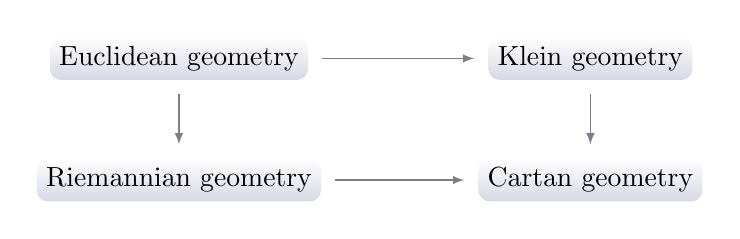
\begin{tikzpicture}[
  cell/.style={%
    rounded corners,
    shade,
    top color=white,
    bottom color=Periwinkle!50!black!20
  },
  line/.style={%
    draw=Periwinkle!30!black!70, thin,
    -latex,
    shorten >=5pt, shorten <=5pt
  }
]
\matrix [column sep=2cm, row sep=1cm]
{%
\node [cell] (eucl) {Euclidean geometry}; &
\node [cell] (klein) {Klein geometry}; \\
\node [cell] (riem) {Riemannian geometry}; &
\node [cell] (cartan) {Cartan geometry}; \\
};
\path [line] (eucl) -- (klein);
\path [line] (eucl) -- (riem);
\path [line] (riem) -- (cartan);
\path [line] (klein) -- (cartan);
\end{tikzpicture}
\caption{%
  Generalization scheme of geometries, where generalization runs 
  along the direction of the arrows. The first row includes 
  homogeneous manifolds in which the symmetry group of Euclidean 
  geometry is generalized to generic Lie groups. The second row 
  are the corresponding nonhomogeneous geometries, which retain 
  the homogeneity of their model geometries at the local level, 
  but which are more general in that they have nonvanishing 
  curvature and torsion. Adapted from~\cite{sharpe1997diff_geo}.
}
\label{fig:gen_scheme_cartan}
\end{figure}

Our review on Cartan geometry principally 
follows~\cite{sharpe1997diff_geo}, a must-read for those who want 
an extended analysis of the subject and some of its applications.  
Further mathematically rigorous discussions on Cartan geometry 
are found in~\cite{kobayashi:1957tc, Alekseevsky:1995cc}, while 
the articles~\cite{Wise:2009fu, Wise:2010sm, Westman:2012xk} are 
helpful for understanding the geometric intuition that underlies 
the abstract notions central to the mathematics. In the 
following, we shall assume that $G$ and $H$ are Lie groups, such 
that $H$ is a subgroup of $G$, and denote their Lie algebras by 
$\mf{g}$ and $\mf{h}$, respectively.

\begin{definition}
A \emph{Cartan geometry} $(P,A)$ modeled on $(\mf{g},H)$ consists 
of a principal $H$ bundle $P(\mc{M},H)$, on which there exists a
$\mf{g}$-valued one-form $A$--- the \emph{Cartan connection}--- 
satisfying the following properties:
\begin{itemize}
  \item[(i)] The map $A : T_p P \to \mf{g}$ is a linear 
    isomorphism, at any $p \in P$;
  \item[(ii)] $A(B^\star) = B$, for each fundamental vector field 
    corresponding to $B \in \mf{h}$;
  \item[(iii)] $R_h^*A = \Ad_{h^{-1}} A$, for every $h \in H$.
\end{itemize}
A Cartan geometry is said to be reductive if $\mf{g} = \mf{h} 
\oplus \mf{p}$, where $\mf{p} = \mf{g}/\mf{h}$, is a reductive 
splitting.
\end{definition}

The Cartan connection differs from an Ehresmann connection in the 
first of its defining properties. Whereas the latter connection 
is valued in the Lie algebra of its structure group, a Cartan 
connection is valued in a larger algebra that must be of the same 
dimension as $P$. This is an important ingredient of Cartan 
geometries, because it implies that the dimension of the base 
manifold is equal to the dimension of the homogeneous space of 
the Klein geometry $(G,H)$, i.e.
\begin{equation*}
  \dim \mc{M} = \dim G/H.
\end{equation*}

The isomorphism $A_p$ can be inverted pointwise to give an 
injection of $\mf{g}$ into $\mathscr{X}(P)$, namely, $A^{-1} 
: B \in \mf{g} \mapsto A_p^{-1}(B) \in T_p P$. The $H$ 
equivariance property of the Cartan connection implies that 
$A_{ph}^{-1} = R_{h*} \circ A_p^{-1} \circ \Ad_h$, as can be 
verified from the following commuting diagram:
\begin{equation*}
\begin{tikzcd}[
  column sep=1.5cm
  ]
  T_pP
    \arrow[r, "R_{h*}"]
    \arrow[d, "A_p"]  &
  T_{ph}P
    \arrow[d, "A_{ph}"]
  \\
  \mf{g}
    \arrow[r, "\Ad_{h^{-1}}"] &
  \mf{g}
\end{tikzcd}%
.
\end{equation*}
Because $A(B^\star) = B$ for each $B \in \mf{h}$ and since
$A$ is a linear isomorphism, one concludes that $A^{-1}(B)$ is 
the fundamental vector field that corresponds to $B \in \mf{h}$.  
At an arbitrary point $p$, the restriction of the Cartan 
connection on the fibres yields
\begin{equation*}
  A_p(B^\star) = B = \omega_H(B^\star),
\end{equation*}
where on the most right-hand side $B^\star$ denotes the 
fundamental vector field on the Lie group $H$. It is in this 
sense that the Cartan connection is said to restrict to the 
Maurer-Cartan form on the fibres of $P$, i.e., $A|_H = \omega_H$.

The \emph{Cartan curvature} is the exterior covariant derivative 
of the Cartan connection, which is given by
\begin{equation}
  \label{eq:Cartan_curv}
  F = dA + \frac{1}{2}[A,A],
\end{equation}
and satisfies the Bianchi identity
\begin{equation}
\label{eq:cartan_bianchi}
  dF + [A,F] \equiv 0.
\end{equation}
The $\mf{g}$-valued two-form $F$ is strictly horizontal in the 
sense that it vanishes if at least one of its arguments is a 
vertical vector field. This can be understood by observing that 
$A$ restricts to $\omega_H$ on the fibres, whose exterior 
covariant derivative is always zero, see~\eqref{eq:MC_struct_eq}.  
Explicitly, it is verified as follows. Since $F$ is a two-form, 
it is enough to check that $F(X^\mrm{v},Y)$ vanishes, where 
$X^\mrm{v}$ is a vertical and $Y$ a generic vector field on $P$.  
At any $p \in P$, there is a $B \in \mf{h}$ such that 
$X^\mrm{v}_p = B^\star_p = A^{-1}_p(B)$.  Thence,
$F_p(X^\mrm{v},Y) = dA_p(A^{-1}_p(B), Y) + [B,A_p(Y)]$, and
\begin{align*}
  dA_p(A^{-1}_p(B), Y)  &= {\big(i_{A^{-1}_p(B)} \circ 
    dA\big)}_p(Y)
  \\
  &= -{\big(d \circ i_{A^{-1}_p(B)} A\big)}_p(Y)  
  + {\big(\mathscr{L}_{A^{-1}_p(B)} A\big)}_p(Y),
\end{align*}
where we used~\eqref{eq:LieExtInt}.
Since $i_{B^\star} A = B$ is a constant function, the first term 
vanishes. If we denote $b_t = \exp(tB)$, the second term can be 
written as $\lim_{t \to 0} \tfrac{1}{t} [ {(R_{b_t}^*A)}_p(Y) 
- A_p(Y)] = - \ad_B(A_p(Y))$. We thus find that what was looked 
for:
\begin{equation*}
F_p(X^\mrm{v},Y) = - \ad_B(A_p(Y)) + \ad_B(A_p(Y)) \equiv 0.
\end{equation*}

A Cartan geometry is said to be \emph{flat} if the Cartan 
curvature vanishes. An example of a flat Cartan geometry modeled 
on $(\mf{g},H)$ is the Klein geometry $(G,H)$. More precisely, 
the pair $(G,\omega_G)$ is a flat Cartan geometry, which can 
easily be verified by comparing the definition for the latter 
with the structure associated with a Klein geometry discussed in 
\S\ref{sec:Klein_geo}. Conversely, the space $\mc{M}$ of a flat 
Cartan geometry modeled on $(\mf{g},H)$ is in the neighborhood of 
any point of $\mc{M}$ isomorphic as a Cartan geometry to an open 
subset of the Klein space $S \simeq 
G/H$~\cite{sharpe1997diff_geo}. The Cartan curvature is thus a 
measure that quantifies the nonhomogeneity of $\mc{M}$, in 
comparison with the perfect homogeneity of the Klein space $S$.

For the following, we restrict our attention to reductive Cartan 
geometries for which, moreover, the Lie algebra $\mf{g}$ is 
symmetric. Concretely, there is a reductive splitting as vector 
spaces
\begin{equation}
  \mf{g} = \mf{h} \oplus \mf{p}
\end{equation}
such that $[\mf{h},\mf{h}] \subseteq \mf{h}$, $[\mf{h},\mf{p}] 
\subseteq \mf{p}$, and $[\mf{p},\mf{p}] \subseteq \mf{h}$. It is 
the last condition that is necessarily fulfilled in order that a 
reductive algebra be symmetric. When the Cartan geometry is 
reductive, it is sensible to consider the corresponding 
decompositions of the connection and its curvature, thus defined 
by
\begin{equation*}
\begin{split}
  A_\mf{h} &= \mrm{pr}_\mf{h} \circ A \\
  A_\mf{p} &= \mrm{pr}_\mf{p} \circ A
\end{split}
\quad\quad\text{and}\quad\quad
\begin{split}
  F_\mf{h} &= \mrm{pr}_\mf{h} \circ F \\
  F_\mf{p} &= \mrm{pr}_\mf{p} \circ F,
\end{split}
\end{equation*}
because they transform reducibly under the right $H$ action.

\begin{proposition}
\label{prop:cartan_ehres_coframe}
The one-form $A_\mf{h} \in \Omega(P,\mf{h})$ is an Ehresmann 
connection on $P$, and the one-form $A_\mf{p} \in 
\Omega(P,\mf{p})$ is a displacement form, namely, $H$ 
equivariant, i.e., $R_h^*A_\mf{p} = \Ad(h^{-1}) A_\mf{p}$ for 
each $h \in H$, and strictly horizontal.
\end{proposition}

\begin{proof}
Because $A$ is $H$ equivariant and since $\mf{g}$ is reductive, 
it follows that $R_h^*A_\mf{h} + R_h^*A_\mf{p} = \Ad(h^{-1}) 
A_\mf{h} + \Ad(h^{-1}) A_\mf{p}$. By rearranging this equation so 
that
\begin{equation*}
  R_h^*A_\mf{h} - \Ad(h^{-1})A_\mf{h}
    = \Ad(h^{-1}) A_\mf{p} - R_h^*A_\mf{p},
\end{equation*}
we obtain an equality between an $\mf{h}$-valued left-hand side 
and a $\mf{p}$-valued right-hand side. This only makes sense if 
both sides vanish, which proves the $H$ equivariance of 
$A_\mf{h}$ and $A_\mf{p}$.

Next let $B^\star$ be the fundamental vector field that 
corresponds to $B \in \mf{h}$. We have that $B = A(B^\star) = 
A_\mf{h}(B^\star) + A_\mf{p}(B^\star)$, or
\begin{equation*}
  B - A_\mf{h}(B^\star) = A_\mf{p}(B^\star).
\end{equation*}
This can only be true if both sides vanish, hence 
$A_\mf{h}(B^\star) = B$ and $A_\mf{p}(B^\star) = 0$, which 
completes the proof.
\end{proof}

Note that for any $B \in \mf{p}$, $A_\mf{h}(A^{-1}(B)) = 0$ as 
$A$ is an isomorphism. Consequently, at any $p \in P$ the 
subspace $A_p^{-1}(\mf{p})$ is horizontal with respect to the 
Ehresmann connection $A_\mf{h}$. Conversely, any element of $H_p$ 
must be in $A_p^{-1}(\mf{p})$, so that at $A_p^{-1}(\mf{p}) = 
H_p$. If $\mf{g}$ is reductive, the distribution $p \to 
A_p^{-1}(\mf{p})$ is right invariant and is therefore equal to 
the horizontal distribution that corresponds to $A_\mf{h}$:
\begin{equation*}
  H_{ph} = A_{ph}^{-1}(\mf{p})
    = R_{h*}A_p^{-1}( \Ad_h( \mf{p}))
    = R_{h*}H_p,
\end{equation*}
This also implies that the tangent spaces of $\mc{M}$ can be 
identified with $\mf{p}$, up to adjoint $H$ transformations, 
because $\pi_* : H_p \to T_x\mc{M}$ is right invariant. Moreover, 
if there is defined an $\Ad(H)$ invariant metric on $\mf{p}$, it 
can be pulled back to give a metric structure on the base 
manifold $\mc{M}$.

The two-forms $F_\mf{h}$ and $F_\mf{p}$ are $H$ equivariant and 
horizontal, because the same is true for $F$, as has been 
verified above. For a symmetric Lie algebra, the definition for 
the Cartan curvature~\eqref{eq:Cartan_curv} allows us to express 
them in terms of $A_\mf{h}$ and $A_\mf{p}$, namely,
\begin{subequations}
\label{eqs:curv_tors_expl}
\begin{align}
  \label{eq:curv_expl}
  F_\mf{h} &= dA_\mf{h} + \frac{1}{2} 
  [A_\mf{h}, A_\mf{h}]  + \frac{1}{2}
  [A_\mf{p},A_\mf{p}],
  \\
\shortintertext{and}
  \label{eq:tors_expl}
  F_\mf{p} &= dA_\mf{p} + 
  [A_\mf{h},A_\mf{p}].
\end{align}
\end{subequations}
The $\mf{h}$-valued $F_\mf{h}$ is called the (corrected) 
curvature of the geometry. In general, this is not the same as 
the exterior covariant derivative of the Ehresmann connection 
$A_\mf{h}$, which is given by $dA_\mf{h} + \frac{1}{2} 
[A_\mf{h}, A_\mf{h}]$ only. The $\mf{p}$-component 
$F_\mf{p}$ of the Cartan curvature is called the \emph{torsion} 
of the geometry. The Klein geometry $(G,H)$ is therefore a Cartan 
geometry modeled on $(\mf{g},H)$ with vanishing curvature and 
torsion.

We also decompose the Bianchi identity~\eqref{eq:cartan_bianchi} 
in an $\mf{h}$-, respectively, $\mf{p}$-valued component, 
rendering the identities
\begin{subequations}
\label{eqs:bianchi_ids_decomp}
\begin{gather}
  d_{A_\mf{h}} \circ d_{A_\mf{h}} A_\mf{h} \equiv 0,\\
\shortintertext{and}
  d_{A_\mf{h}} \circ d_{A_\mf{h}} A_\mf{p} + [A_\mf{p}, 
  d_{A_\mf{h}} A_\mf{h}] \equiv 0,
\end{gather}
\end{subequations}
where $d_{A_\mf{h}}$ is the exterior covariant derivative with 
respect to the Ehresmann connection~$A_\mf{h}$.

The structures associated with a Cartan connection were 
heretofore all considered on the bundle space $P$ only. As we 
already mentioned in \S\ref{sec:Ehresmann_conn}, it is necessary 
to pull back the geometric objects to the base manifold, for it 
is here that physical theories are implemented in a concrete 
manner. Just as an Ehresmann connection and its curvature are 
pulled back by a family of gauges $\sigma$, a Cartan connection 
and its curvature give rise to a family of local connection and 
curvature forms, defined on subdomains of $\mc{M}$. These local 
forms will be denoted by the same symbols as the corresponding 
forms on $P$.  Furthermore, from the transformation behavior of 
the Cartan connection and its curvature under gauge 
transformations $\sigma \mapsto \sigma' = \sigma h^{-1}$, one 
concludes that the local connection $A$ and curvature $F$ 
transform as
\begin{equation}
\label{eq:trafoLocalCartanConnCurv}
  A \mapsto \Ad(h) A + h^{-1*}\omega_H
  \quad\text{and}\quad
  F \mapsto \Ad(h) F,
\end{equation}
where $h^{-1*}\omega_H = hdh^{-1}$ if $H$ is a matrix group. We 
conclude in mentioning that the $\mf{p}$-valued part of the local 
connection, i.e., $A_\mf{p} : T_x \mc{M} \to \mf{p}$ is an 
isomorphism. This follows from the first condition in the 
definition of a Cartan connection. Naturally, such an isomorphism 
only makes sense for reductive Cartan geometries.


\section{Relation between Ehresmann and Cartan connections}
\label{sec:relEhrCartConns}

In this final section on Cartan geometry we discuss the 
relationship between Ehresmann connections and Cartan 
connections.  To be precise, we shall review how certain 
Ehresmann connections on a principal $G$ bundle restrict to 
Cartan connections modeled on $(\mf{g},H)$ on a reduced $H$ 
bundle.

The reduction of a principal $G$ bundle to a principal bundle 
with structure group $H$, $H$ being a subgroup of $G$, comes down 
to the restriction of the structure group $G$ to the smaller 
group $H$, as will be reviewed in \S\ref{ssec:reduction_bundle}.  
At various places in physics, such a mechanism generally models 
a situation in which a larger symmetry group is broken down to an 
enclosed group describing less symmetry. Such a reduction of 
symmetries may be forced by hand or may happen by chance, which 
is the case in spontaneous symmetry breaking.

We already saw that the notion of symmetry breaking is closely 
related to the Lie theoretic description of homogeneous spaces in 
Klein geometry, where the isomorphism $S \simeq G/i(H)$ depends 
on the inclusion $i : H \to G$, $i(H) = H_\xi$ being the isotropy 
group of an arbitrary point $\xi$ in $S$. In a similar way, a 
principal $G$ bundle reduces to a principal $H$ bundle by 
singling out a section $\xi$ of the associated $G$ bundle with 
typical fibre $S$. Conceptually, the section $\xi$ locally 
singles out a point $\xi(x)$ of the fibre $S_x$ over $x$, which 
breaks the symmetry group $G$ of $S$ pointwise to $i_x(H) = 
H_{\xi(x)}$.  Concomitantly, some Ehresmann connections on the 
$G$ bundle restrict to Cartan connections on the reduced $H$ 
bundle.  A rather rigorous discussion of this reduction process 
is indispensable to understand how the accompanying breakdown of 
symmetry can be recovered by observing that the choice of section 
$\xi$ is completely arbitrary, an observation that will be of use 
in~\S\ref{sec:nonlindSCgeometry}.

\subsection{Reduction of principal fibre bundles}
\label{ssec:reduction_bundle}

Our short synthesis on the reduction of principal bundles is 
based on the work~\cite{kob1996found, husemoller:1966fibre, 
  husemoller.etal:2008bbt}, but the notation used here is 
slightly adapted so that it will be easier to make connection 
with its role played later on in this dissertation.

\begin{definition}
Let $P(\mc{M},H)$ be a principal $H$ bundle and $Q(\mc{M},G)$ a 
principal $G$ bundle over the same base manifold $\mc{M}$, such 
that $i_x : H \to G$ is an inclusion, i.e., an injective 
homomorphism, for each $x \in \mc{M}$.  Let $\imath : P \to 
\imath(P) \subset Q$ be a homeomorphism such that
\begin{equation*}
  \imath(ph) = \imath(p) i_x(h)
  \quad\text{and}\quad
  \pi_Q \circ \imath = \pi_P,
  \quad\text{where}~%
  x = \pi_P(p).
\end{equation*}
We then say that $P$ is a \emph{reduction} of $Q$ and that the 
structure group $G$ is reduced to the group $H \simeq i_x(H)$, 
while $Q$ is called an \emph{extension} of $P$.
\end{definition}

Note that the inclusion $i_x$ varies along $\mc{M}$, but that 
each $i_x(H)$ is isomorphic with any other, so that the 
definition makes sense. Because $i_x(H)$ is a subgroup of $G$ we 
can construct the space $Q/i_x(H)$ of equivalence classes $[q] 
= [q\, i_x(h)]$, where $\pi_Q(q) = x$.  We denote the canonical 
projection of $Q$ onto the space of equivalence classes by
\begin{equation*}
  \mu_x : q \in Q \mapsto [q] \in \frac{Q}{i_x(H)}.
\end{equation*}
Just as we could identify a space $S$ that is symmetric under $G$ 
with the space of cosets $G/H_\xi$, where $H_\xi$ is the group 
leaving $\xi$ fixed, it is possible to identify the associated 
bundle $Q \times_G S$ with the space of equivalence classes 
$Q/i_x(H)$, where $i_x(H) = H_{\xi(x)}$ for any $x = \pi_Q(q)$, 
namely,
\begin{equation*}
  [q,a\xi] \in Q \times_G S
  \rightleftharpoons
  [qa] \in \frac{Q}{i_x(H)}.
\end{equation*}
This is a well-defined identification, for $[qa] = [qa\, i_x(h)] 
\rightleftharpoons [qa, i_x(h) \xi] = [qa, \xi]$.

Given a principal $H$ bundle $P(\mc{M},H)$, we always can extend 
it to a principal $G$ bundle as follows. Consider the associated 
fibre bundle $Q = P \times_{i_x(H)} G$, where $x = \pi_P(p)$, 
which consists of the equivalence classes $[p,g] = [ph,i_x(h)g]$.  
The manifold $Q$ is turned into a principal fibre bundle over 
$\mc{M}$ with structure group $G$ by including the right $G$ 
action, naturally defined by $[p,g]g' = [p,gg']$. The right 
action on the space of equivalence classes $Q = P[G]$ is well 
defined, because it commutes with the left action, i.e.,
\begin{equation*}
  [p,g]g' = [ph,i_x(h)g]g' = [ph,i_x(h)gg'] = [p,gg'].
\end{equation*}
The extension is then constructed by
\begin{equation*}
  \imath : p \in P \mapsto [p,e] \in Q = P \times_{i_x(H)} G.
\end{equation*}

On the other hand, it is generally not possible to reduce a 
principal bundle $Q(\mc{M},G)$ to a principal $H$ bundle. This is 
the subject of study in the following proposition.

\begin{proposition}
A principal bundle $Q$ with structure group $G$ is reducible to a 
principal bundle $P$ with structure group $H$, if and only if the 
associated bundle $Q[S]$, where $S \simeq G/H$, admits a globally 
defined section.
\end{proposition}

\begin{proof}
First assume that $\imath : P \to Q$ is a reduction. The composed 
mapping $\tilde{\sigma} = \mu_x \circ \imath : P \to Q/i_x(H) 
\simeq Q[S]$ is constant on the fibres of $P$, since for every $h 
\in H$
\begin{equation*}
  \mu_x(\imath(ph)) = \mu_x(\imath(p) i_x(h))
  = \mu_x(\imath(p)).
\end{equation*}
Hence, the mapping $\sigma = \tilde{\sigma} \circ \pi^{-1}_P 
: x \in \mc{M} \mapsto \tilde{\sigma}(p) \in Q[S]$ is a section, 
because
\begin{equation*}
  \pi_{Q[S]}(\sigma(x)) = \pi_{Q[S]}(\tilde{\sigma}(p)) = 
  \pi_{Q[S]}([\imath(p),\xi]) = \pi_Q(\imath(p)) = x,
\end{equation*}
so that $\pi_{Q[S]} \circ \sigma = \mathrm{id}_\mc{M}$.

Conversely, let $[q,\xi]$ be a section of $Q[S]$.  According to 
Prop.~\ref{prop:corr_sec_map}, there is a corresponding $G$ 
equivariant mapping $\varphi : Q \to S$ such that $\xi 
= \varphi(q)$. Consider the subspace of $Q$, given by
\begin{equation*}
  \imath(P) = \{ q \in Q \mid q = \varphi^{-1}(\xi) 
  \text{~if~}\pi_Q(q) = \pi_{Q[S]}([q,\xi]) \}.
\end{equation*}
Denote by $\pi_P$ the restriction of $\pi_Q$ on $\imath(P)$ and 
let $q_1$ and $q_2$ be elements of $\pi^{-1}_P(x)$ for some $x 
\in \mc{M}$. It follows that $\xi = \varphi(q_1) = \varphi(q_2)$ 
and that there exists an element $g \in G$ such that $q_1 
= q_2g$.  Because $\varphi$ is $G$ equivariant, we have that $\xi 
= g\xi$, so that $g \in i_x(H)$, where $i_x(H)$ is the fixed 
group of $\xi$. Therefore, the structure group of $\imath(P)$ is 
everywhere isomorphic with $H$ and $\imath : P \to Q$ is 
a reduction from the structure group $G$ to $i_x(H) \simeq H$.
\end{proof}

To conclude, we summarize the reduction process diagrammatically 
in Fig.~\ref{fig:diagram_reduction}.
\begin{figure}
\centering
$
\begin{tikzcd}[
  row sep=0.3cm,
  column sep=2cm
  ]
  {}  & & S \simeq G/H
  \\
  P(\mc{M},H)
    \arrow[r, "\imath" color=BrickRed]
    \arrow[ddr, end anchor=north west]
  &  Q(\mc{M},G)
    \arrow[
      ur, "\varphi",
      start anchor={[yshift=-4pt]north east}]
    \arrow[dr, "\mu_x",
      start anchor={[yshift=+4pt]south east}]
    \arrow{dd}
  \\
  {}  & & Q \times_G S
    \arrow[dl, end anchor=north east]
  \\
  {}  & \mc{M}
    \arrow[ur, "\sigma" color=BrickRed,
      dashed, swap,
      bend right=15,
      start anchor={[xshift=+2pt]real east},
      end anchor={[xshift=+5pt]south west}]
\end{tikzcd}
$
\caption{The diagram summarizes which manifolds take part in the 
  reduction process and how they are related by the different 
  mappings discussed in the text. The reductions $\imath$ are in 
  one-onto-one correspondence with the sections $\sigma$.}
\label{fig:diagram_reduction}
\end{figure}

\subsection{Restricting Ehresmann to Cartan connections}

Consider a reduction $\imath : P \to Q$ from a principal $G$ 
bundle to a principal $H$ bundle such that the dimension of $P$ 
equals $G$. The following proposition specifies which Ehresmann 
connections on $Q$ are pulled back by the reduction to Cartan 
connection on $P$.

\begin{proposition}
Let $\omega \in \Omega(Q,\mf{g})$ be an Ehresmann 
connection on $Q$. If
\begin{equation}
\label{eq:cond_reduc_Cartan}
  \ker\omega \cap \imath_\ast(TP) = 0,
\end{equation}
then the one-form $A \in \Omega(P,\mf{g})$ defined by
\begin{equation*}
  A = \imath^\ast\omega
\end{equation*}
is a Cartan connection on $P$.
\end{proposition}

\begin{proof}
Because $\ker\omega_p \cap \imath_\ast(T_p P)$ is zero for every 
$p$, $\imath^\ast\omega = \omega\circ\imath_\ast$ is 
a $\mf{g}$-valued one-form on $P$ that has no kernel.
\begin{itemize}
  \item[(i)] Because $\imath$ is an injection and the dimension 
    of $P$ and $G$ are equal, $\imath^\ast\omega$ is an 
    isomorphism at every $p$;
  \item[(ii)] Let $B^\star$ be the fundamental vector field on 
    $P$ that corresponds to $B \in \mf{h}$, namely, for each 
    function $f$ we have $B^\star f = df(p b_t)/dt$, where $b_t 
    = \exp(tB)$. It follows that
    \begin{equation*}
      (\imath_\ast B^\star) f
      = \frac{d}{dt} f(\imath(p) i_x(b_t)),
      \quad\text{where}~%
      x = \pi_P(p),
    \end{equation*}
    which is fundamental vector field on $Q$ corresponding to $B 
    \in \mf{h}$. It follows that $\imath^\ast\omega(B^\star) = B$ 
    for each $B \in \mf{h}$.
  \item[(iii)] For any $p$ it is true that $\imath \circ R_h (p) 
    = \imath(p) i_x(h) = R_{i_x(h)} \circ \imath (p)$, where $x = 
    \pi_P(p)$. Therefore,
    \begin{equation*}
      {(R_h^* \imath^*\omega)}_{p}
      = {\big(\imath^* R_{i_x(h)}^* \omega\big)}_p
      = \Ad(i_x(h)) {(\imath^* \omega)}_p.
    \end{equation*}
\end{itemize}
By identifying $i_x(H) \simeq H$ at any $x \in \mc{M}$, this 
proves that $A = \imath^* \omega$ is a Cartan connection on 
$P(\mc{M},H)$.
\end{proof}

We have seen above that there is a one-onto-one correspondence 
between reduction $\imath : P \to Q$ and section from the 
associated bundle $Q[S] = Q \times_G S$. Therefore, a Cartan 
connection on $P$ can be thought as an Ehresmann connection on 
$Q$ together with a section of $Q[S]$ for which the corresponding 
reduction satisfies~\eqref{eq:cond_reduc_Cartan}.


\chapter{Cartan geometry of spacetimes with a nonconstant 
  cosmological function}
\label{ch:dSC_geometry}

The means of Cartan geometry now at our disposal, we next present 
the geometry of spacetimes that are tangentially approximated by 
de Sitter spaces whose cosmological constants vary over 
spacetime~\cite{Jennen:2014mba}. For this purpose we consider 
a Cartan geometry for which the local Klein space is at each 
point a de Sitter space, but for which the combined set of 
pseudoradii forms a nonconstant function on spacetime.  We begin 
with a study of de Sitter space as a metric Klein geometry, after 
which de Sitter--Cartan spacetimes with a cosmological function 
are introduced. We show that the torsion of such geometries 
receives a contribution that is not present for a cosmological 
constant.  The structure group of the obtained de~Sitter--Cartan 
geometry is by construction the Lorentz group~$SO(1,3)$.  
Invoking the theory of nonlinear realizations, we extend the 
class of symmetries to the enclosing de~Sitter group~$SO(1,4)$, 
and compute the corresponding spin connection, vierbein, 
curvature, and torsion.

\section{Klein geometry of de Sitter space}
\label{sec:Klein_dS_space}

Four-dimensional de Sitter space $dS$ is a spacetime that is 
visualized easiest by embedding it as the hyperboloid\footnote{We 
  use the convention $\eta_{AB} = \mrm{diag}(+1, -1, -1, -1, 
  -1)$; see also 
  \S\ref{sapp:Lorentz_group}.}~\cite{hawking:1973ls,Spradlin:2002ds}
\begin{equation*}
  \eta_{AB} \chi^A \chi^B = -\frac{3}{\Lambda}
  \quad\text{with}~\Lambda > 0
\end{equation*}
in the five-dimensional vector space $\mathds{R}^{1,4}$ 
parametrized by Cartesian coordinates, see 
Fig~\ref{fig:dSembedded}. The number $\Lambda$ is the 
cosmological constant of Einstein's equations~\cite{Wald:1984gr}, 
for which there is a different de Sitter space for every positive 
value of the cosmological constant. In what follows we shall 
discuss de Sitter space explicitly from the Lie theoretic point 
of view offered by metric Klein geometry, see 
also~\cite{kob1996found2,Wise:2010sm} and~\S\ref{sec:Klein_geo}.  
Such a treatment allows us to relate the cosmological constant of 
$dS$ to a length scale defined in the translational part of the 
Lie algebra $\mf{so}(1,4)$. This relation will be important when 
we define spacetimes with a nonconstant cosmological function 
in~\S\S\ref{sec:dSCgeometry}--\ref{sec:nonlindSCgeometry}.

\begin{figure}
\iftoggle{draftVersion}{%
  \framebox[7cm][c]{%
    \textbf{XXX} Figure: de Sitter space}
}{% else
\centering
\begin{tikzpicture}[scale=1.5]
\def\l{1}
\begin{axis}[
  anchor=origin,
  xmin=-1.8, xmax=1.8,  % \chi_4
  ymin=-1.8, ymax=1.8,  % \chi_3
  zmin=-3, zmax=3,      % \chi_0
  xlabel=$\chi^4$,
  zlabel=$\chi^0$,
  axis equal,
  hide axis,
  view={0}{20},
  colormap name={Set3-3}
  %colormap name={RdGy-3}
  %colormap name={PuBu-3} % colorbrew library
  ]
  % x = \tau ; y = \phi
  \addplot3[
    surf,
    samples=50,
    samples y=35,
    domain=-1.7:1.7, y domain=0:2*pi
    ]({\l*cosh(x/\l)*cos(deg(y))},
      {\l*cosh(x/\l)*sin(deg(y))},
      {\l*sinh(x/\l)});
\end{axis}
\draw[-stealth] (1.25,-0.5) -- (1.25,0.5);
\node at (1.25,0) [anchor=west] {$\chi^0$};
\end{tikzpicture}
}% end \iftoggle
\caption{Two-dimensional hyperboloid illustrating a de Sitter 
  space with two spacelike dimensions suppressed. The constant 
  time slices represent three-spheres $S^3$ with time-dependent 
  radii.}
\label{fig:dSembedded}
\end{figure}

The group $SO(1,4)$ acts transitively and effectively on de 
Sitter spaces with arbitrary cosmological constants, a standard 
result proven in~\cite{kob1996found}, for example. The Lorentz 
group in five dimensions is therefore also called the \emph{de 
  Sitter group}.  Hence, the de Sitter group is the symmetry 
group of de Sitter space and the pairs $(dS,SO(1,4))$ form a set 
of homogeneous spaces, namely, one for each $\Lambda$. According 
to \S\ref{sec:Klein_geo}, in order to describe $dS$ in terms of 
its symmetry group is it necessary to single out an origin $o$, 
which we choose to be the south pole, i.e., the point with 
coordinates $o^A = (0, 0, 0, 0, -\sqrt{3/\Lambda})$.  The 
isotropy group of the south pole consists of the elements of the 
de Sitter group that are of the form,
\begin{equation}
\label{eq:SO(1,3)_o_isotropy}
  \Lambda\ind{^A_B} =
\begin{pmatrix}
  \Lambda\ind{^a_b} & 0 \\
  0     & 1
\end{pmatrix},
\quad
\text{where}~\Lambda\ind{^a_b} \in SO(1,3).
\end{equation}

The fixed group of the origin is manifestly isomorphic to the 
Lorentz group in four dimensions, whereas the matrix above 
clearly illustrates the inclusion ${SO(1,3)}_o = i(SO(1,3)) 
\subset SO(1,4)$.  Because the action of the de Sitter group on 
$dS$ is transitive, coset elements of $SO(1,4)/{SO(1,3)}_o$ are 
in one-onto-one correspondence with points of de Sitter space, 
namely, there is the isomorphism
\begin{equation}
\label{eq:isom_cosets_dS}
  \lambda_o : [\Lambda\ind{^A_B}] \in \frac{SO(1,4)}{{SO(1,3)}_o}
  \mapsto
  \chi^A = \Lambda\ind{^A_B} o^B \in dS.
\end{equation}
We shall denote the inclusion ${SO(1,3)}_o$ by $SO(1,3)$ as well, 
so that it has been verified that $(SO(1,4),SO(1,3))$ is an 
effective Klein geometry, wherein the Klein space is isomorphic 
to the de Sitter space, i.e., $SO(1,4)/SO(1,3) \simeq dS$. Note 
however that the left-hand side of this isomorphism does not make 
reference to the cosmological constant of the right-hand side.  
Therefore, the present description offered by Klein geometry is 
not sufficient if we want to discriminate between de Sitter 
spaces with different values for $\Lambda$. In concordance with 
\S\ref{sec:Klein_geo} we extend the structure to a metric Klein 
geometry in order to introduce metrical properties on the Klein 
space. To do so, it is necessary to shift focus to the 
infinitesimal structure of the principal group, namely, to its 
Lie algebra, as follows.

To begin with, it should be observed that the Klein geometry 
$(SO(1,4),SO(1,3))$ is a symmetric space. To be precise, in 
concordance with the definition of symmetric 
spaces~\cite{kob1996found2, loos:1969ss}, there is an involutive 
automorphism $\sigma$ on $SO(1,4)$ induced by the linear 
transformation $S\ind{^A_B} : (\chi^a,\chi^4) \mapsto 
(-\chi^a,\chi^4)$, which in the fundamental representation acts 
according to
\begin{equation*}
  \sigma(\Lambda)\ind{^A_B} = S\ind{^A_C} \Lambda\ind{^C_D} 
  S\ind{^D_B},
  \quad
  S\ind{^A_B} =
  \begin{pmatrix}
    -\mathds{1}_{4} & 0 \\
    0         & 1
  \end{pmatrix}.
\end{equation*}
From~\eqref{eq:SO(1,3)_o_isotropy} one sees that the Lorentz 
subgroup is invariant under the action of $\sigma$. This 
automorphism on $SO(1,4)$ induces a corresponding automorphism on 
the algebra $\mf{so}(1,4)$, which obviously is given by the 
adjoint action as well. Because $\sigma$ is involutive, the 
vector space $\mf{so}(1,4)$ can be separated in an eigenspace 
$\mf{h}$ with eigenvalue 1 and an eigenspace $\mf{p}$ with 
eigenvalue $-1$, from which it furthermore follows that
\begin{equation*}
  [\mf{h},\mf{h}] \subseteq \mf{h},
  \quad
  [\mf{h},\mf{p}] \subseteq \mf{p},
  \quad\text{and~}
  [\mf{p},\mf{p}] \subseteq \mf{h},
\end{equation*}
for $\sigma$ commutes with the Lie bracket. Since the elements of 
the Lorentz subgroup remain invariant under $\sigma$, 
$\mf{so}(1,3) \subset \mf{h}$. In fact, in its fundamental 
representation elements of the de Sitter algebra are of the form
\begin{align}
\notag
  \omega\ind{^A_B} &=
  \begin{pmatrix}
    \omega\ind{^a_b}  & 0 \\
    0           & 0
  \end{pmatrix}
  -
  \begin{pmatrix}
    0_4           & \omega^a/l \\
    \omega_a/l    & 0
  \end{pmatrix},
  \\
\label{eq:red_split_SO14_fund}
  &= \frac{i}{2} \omega^{ab} [M_{cd}]\ind{^a_b} + i \omega^b 
  [P_b]\ind{^a_4},
\end{align}
with $\omega^a = -l\omega\ind{^a_4}$ and $\omega_a = \eta_{ab} 
\omega^b$, and where the $M_{ab}$ span the Lorentz algebra while 
the $P_a = M_{a4}/l$ the linear complement $\mf{p} 
=\mf{so}(1,4)/\mf{so}(1,3)$, which are called the infinitesimal 
\emph{de Sitter translations} or \emph{transvections}. It is easy 
to check that $\mf{p}$ is the eigenspace of $\sigma$ with 
eigenvalue $-1$, so that $\mf{h} = \mf{so}(1,3)$ and
\begin{equation}
\label{eq:red_split_so14}
  \mf{so}(1,4) = \mf{so}(1,3) \oplus \mf{p}
\end{equation}
is the corresponding Cartan decomposition~\cite{kob1996found2}. 

The symmetric nature of the de Sitter algebra just verified in 
the fundamental representation can be observed in a way that does 
not depend on the representation, when we decompose the 
commutation relations~\eqref{eq:comm_rel_so(1,d)} for 
$\mf{so}(1,4)$ according to the reductive 
splitting~\eqref{eq:red_split_so14}:
\begin{subequations}
\label{eq:comm_relations_so(1,4)}
\begin{align}
  -i[M_{ab},M_{cd}] &= \eta_{ac}M_{bd} - \eta_{ad}M_{bc} + 
  \eta_{bd}M_{ac} - \eta_{bc}M_{ad}, \\
  -i[M_{ab},P_c] &= \eta_{ac}P_b- \eta_{bc}P_a, \\
\label{eq:comm_relations_so(1,4)C}
  -i[P_a,P_b] &= -l^{-2}M_{ab}.
  \end{align}
\end{subequations}
Similarly to the decomposition~\eqref{eq:red_split_SO14_fund} in 
the fundamental representation, an element $\omega$ of 
$\mf{so}(1,4)$ may be decomposed according to the reductive 
splitting~\eqref{eq:red_split_so14} as $\tfrac{i}{2} \omega^{ab} 
M_{cd} + i \omega^a P_a$, which naturally is invariant under the 
action of the Lorentz group. To obtain an expression for the 
Lorentz action on $\mf{so}(1,4)$ that is independent of the 
representation employed, it is useful to compute it first for the 
fundamental representation. More precisely, if $\omega 
= \tfrac{i}{2} \omega^{AB} M_{AB}$ is an element of the de Sitter 
algebra in a generic representation, we would like to find an 
explicit expression for the components $\tfrac{i}{2} 
{[\Ad(\Lambda)(\omega)]}^{AB}$ in
\begin{align*}
  \Ad(\Lambda)(\omega)
  &= \frac{i}{2} {[\Ad(\Lambda)(\omega)]}^{AB} M_{AB}
  \\
  &= \frac{i}{2} {[\Ad(\Lambda)(\omega)]}^{ab} M_{ab}
  + i {[\Ad(\Lambda)(\omega)]}^a P_a.
\end{align*}
These components are clearly independent of the representation, 
so that they can be found through computing the adjoint action in 
the fundamental representation. Doing so, one obtains that
\begin{equation}
  {[\Ad(\Lambda)(\omega)]}^{ab} = \Lambda\ind{^a_c} 
  \omega\ind{^{cd}} \Lambda\ind{^b_d}
  \quad\text{and}\quad
  {[\Ad(\Lambda)(\omega)]}^a = \Lambda\ind{^a_b} \omega^a.
\end{equation}
This way, we have an expression for the adjoint action on the de 
Sitter algebra for any representation, whereas the part that 
depends on the representation is contained in the form of the 
generators $M_{ab}$ and $P_a$. Note how $\omega^{ab}$ and 
$\omega^a$ do not mix under the adjoint action, which reflects 
the reductive nature of the de Sitter algebra.

We are now in the position to implement the isomorphism between 
the infinitesimal de Sitter translations $\mf{p}$ and the tangent 
space to $dS$ at the origin. This isomorphism is canonically 
given as the pushforward of the isomorphism between 
$SO(1,4)/SO(1,3)$ and de Sitter space, explicitly written out 
in~\eqref{eq:isom_cosets_dS}. With every $i\xi^a P_a \in \mf{p}$ 
we identify an element of $T_o dS$ given by (let $f \in 
\mathscr{F}(dS)$)
\begin{align*}
  \lambda_{o*} \left.\frac{d}{dt}\right|_0 f( \exp(it\xi^a P_a))
  &= \left.\frac{d}{dt}\right|_0 f( \lambda_o(\exp(it\xi^a P_a)))
  \\
  &= \left.\frac{d}{dt}\right|_0 {[ \lambda_o(\exp(it\xi^a 
    P_a))]}^A \left.\frac{\pd}{\pd \chi^A}\right|_o f
\end{align*}
where
\begin{equation*}
  \lambda_o(\exp(it\xi^a P_a))
  = \exp(it \xi^a [P_a]\ind{^A_B})o^B = -
  \begin{pmatrix}
    0 \\ 0 \\ 0 \\ 0 \\ \sqrt{3/\Lambda}
  \end{pmatrix}
  + \frac{1}{l} \sqrt{\frac{3}{\Lambda}}
  \begin{pmatrix}
    \xi^0 \\ \xi^1 \\ \xi^2 \\ \xi^3 \\ 0
  \end{pmatrix}
  t
  + \mc{O}(t^2).
\end{equation*}
Consequently, the isomorphism takes the explicit form given by
\begin{equation}
\label{eq:isom_mf(p)_TdS}
  i\xi^a P_a \in \mf{p} \mapsto
  \frac{1}{l} \sqrt{\frac{3}{\Lambda}} \xi^a \left.\frac{\pd}{\pd 
      \chi^a}\right|_o \in T_o dS.
\end{equation}
Observe how the precise relation between corresponding elements 
depends upon the length scale $l$, introduced above in the 
algebra of de Sitter translations. We will leave the value of $l$ 
arbitrary for the moment, and first consider its role in the 
metrical properties of the Klein geometry.

To provide the Klein space with a metric structure, according to 
\S\ref{sec:Klein_geo} an $\Ad(SO(1,3))$ invariant metric must be 
introduced on $\mf{p}$. Such a metric is given naturally when 
restricting the Killing form of $\mf{so}(1,4)$ to $\mf{p}$.
For any two elements $X$ and $Y$ in $\mf{so}(1,4)$, the Killing 
form is given by $B(X,Y) = 4 \tr (XY)$~\cite{helgasson:1978dg}.  
Therefore, upon restricting this form to $\mf{p}$ we find
\begin{equation*}
  B(i \xi \cdot P, i\vartheta \cdot P)
  = 4[i \xi \cdot P]\ind{^A_B} [i \vartheta \cdot P]\ind{^B_A}
  = \frac{8}{l^2} \eta_{ab} \xi^a \vartheta^b,
\end{equation*}
which is a dimensionless number. Because we would like the inner 
product on $\mf{p}$ to result in a quantity with a dimension of 
length squared, we make use of the length scale $l$ to define the 
symmetric bilinear form $\eta = (l^2/8) B : \mf{p} \times \mf{p} 
\to \mathds{R}$, so that
\begin{equation*}
  \eta(i\xi \cdot P, i\vartheta \cdot P) = \eta_{ab} \xi^a 
  \vartheta^b.
\end{equation*}

The isomorphism~\eqref{eq:isom_mf(p)_TdS} induces a corresponding 
metric on the tangent space at the origin of $dS$.  More 
precisely,  let $g = \lambda_o^{-1*}\eta : T_o dS \times T_o dS 
\to \mathds{R}$ so that
\begin{equation*}
  g(\xi \cdot \pd,\vartheta \cdot \pd)
  = \frac{l^2\Lambda}{3} \eta (i\xi \cdot P, i\vartheta \cdot P) 
  = \frac{l^2\Lambda}{3} \eta_{ab} \xi^a \vartheta^b.
\end{equation*}
This line element should be compared with the metric on $dS$ that 
is induced by the geometry of the embedding vector space 
$\mathds{R}^{1,4}$.  Since the latter is given by 
$\eta_{ab}\xi^a\vartheta^b$, it is manifest that the metrical 
properties of the Klein space $SO(1,4)/SO(1,3)$ coincide with the 
geometry of a corresponding de Sitter space with cosmological 
constant $\Lambda$ if and only if we set the length scale 
introduced in the Lie algebra of de Sitter translations $\mf{p}$ 
according to~\cite{Wise:2010sm}
\begin{equation}
\label{eq:rel_l_Lambda}
  l = \sqrt{\frac{3}{\Lambda}}.
\end{equation}

\section{de Sitter--Cartan geometry}
\label{sec:dSCgeometry}

In \S\ref{ch:Cartan_geo} we saw how Cartan geometries generalize 
homogeneous model Klein spaces to nonhomogeneous spaces with 
arbitrary curvature and torsion, while preserving the homogeneity 
of the model space at the infinitesimal scale of the manifold, 
when the latter is equipped with an adequate Cartan connection.

In this section we construct the Cartan geometry $(P,A)$ that is 
modeled on $(\mf{so}(1,4),\allowbreak SO(1,3))$, where $P$ is 
a principal Lorentz bundle over spacetime $\mc{M}$ and $A$ is an 
$\mf{so}(1,4)$-valued Cartan connection. The homogeneous model 
space for this geometry is de Sitter space, whereas the 
corresponding Klein geometry described in 
\S\ref{sec:Klein_dS_space} is an example of the Cartan geometry 
with vanishing curvature and torsion. The spacetime thus obtained 
describes a four-dimensional nonhomogeneous universe whose 
geometry at the infinitesimal scale reduces to the geometry of de 
Sitter space, which in this sense are called \emph{tangent} de 
Sitter spaces. For such a spacetime local kinematics is governed 
by the de Sitter group, something that will be made concrete 
in~\S\ref{ch:dSTG}.

The cosmological constants of the de Sitter spaces tangent to 
spacetime are determined by a length scale in the de Sitter 
algebra wherein the Cartan connection is valued. By letting this 
length scale be spacetime-dependent in an arbitrary way, with the 
only restriction of forming a smooth function, we shall obtain 
a geometry in which the cosmological constants of the local de 
Sitter spaces vary correspondingly. Doing so, there will be 
defined a nonconstant \emph{cosmological function} $\Lambda$ on 
spacetime from the outset. We shall call the Cartan geometry 
obtained in the manner just outlined a \emph{de Sitter--Cartan 
  geometry}~\cite{Jennen:2014mba}.

In the present section we focus in a rather abstract manner on 
the basic ingredients of a de Sitter--Cartan geometry with 
a nonconstant cosmological function. More precisely, the 
structure group $SO(1,3)$ is considered abstractly a subgroup of 
$SO(1,4)$ without explicitly making reference to the point of 
$dS$ of which it is the isotropy group, whereas the de 
Sitter--Cartan connection will be decomposed according to the 
corresponding reductive splitting. Such a treatment is 
mathematically correct but not explicit enough if we would like 
to interpret the Cartan connection on the Lorentz bundle $P$ as 
an Ehresmann connection on an extended de Sitter bundle $Q$ 
together with a section in the associated bundle $Q[dS]$ of de 
Sitter spaces. In such an interpretation the structure group 
$SO(1,3) \simeq \pi_P^{-1}(x)$ above each $x \in \mc{M}$ is given 
by the isotropy group of the point in $dS \simeq \pi_E^{-1}(x)$ 
singled out by the given section. For the moment we shall not 
enter into further details on this issue, and come back to it in 
the following section. Let us nonetheless emphasize that the 
geometric structure here outlined is complete, and that the spin 
connection, vierbein, curvature and torsion of this section can 
also be seen as gauge-fixed versions of the corresponding objects 
calculated in the section hereafter, as will become clear there. 

A de Sitter--Cartan geometry is thus constructed over spacetime 
$\mc{M}$ when we introduce a $\mf{so}(1,4)$-valued Cartan 
connection $A$, which may be decomposed with respect to the 
reductive splitting~\eqref{eq:red_split_so14} as
\begin{equation}
\label{eq:CartConn_decomp}
  A = A_{\mf{so}(1,3)} + A_\mf{p}
  = \frac{i}{2} A^{ab} M_{ab} + i A^a P_a.
\end{equation}
Under the local Lorentz transformation $\Lambda$ the Cartan 
connection transforms according to (see 
Eq.~\eqref{eq:trafoLocalCartanConnCurv})
\begin{equation*}
  A \mapsto \Ad(\Lambda) A + \Lambda d\Lambda^{-1}.
\end{equation*}
Proposition~\ref{prop:cartan_ehres_coframe} implies that the
$\mf{so}(1,3)$-valued part of $A$ is an Ehresmann connection for 
the Lorentz bundle $P$, i.e., a spin connection. This can also be 
seen directly from the transformation behavior of its components:  
\begin{equation*}
  A\ind{^a_b} \mapsto \Lambda\ind{^a_c} A\ind{^c_d} 
  \Lambda\ind{_b^d} + \Lambda\ind{^a_c} d\Lambda\ind{_b^c}.
\end{equation*}
From now on we shall refer to $A\ind{^a_b}$ as the spin 
connection of the geometry. While this is correct for the 
fundamental representation, it must be remembered that the spin 
connection in an arbitrary representation is really given by 
$\tfrac{i}{2} A^{ab} [M_{ab}]\ind{^\alpha_\beta}$.

The $\mf{p}$-valued one-form $A_\mf{p}$ is called the 
\emph{coframe field} and constitutes a pointwise mapping between 
tangent vectors and infinitesimal de Sitter translations.  This 
mapping induces another map that will be denoted by the same 
symbol as well as given the same name of coframe 
field,\footnote{A comment should be made here to clarify some 
  mathematical subtleties regarding what is meant by the coframe 
  field~\cite{Wise:2010sm}. The form we denoted hitherto by 
  $A_\mf{p}$ is a pulled-back version of the $\mf{p}$-valued part 
  of the Cartan connection $A : TP \to \mf{so}(1,4)$ 
  from~\S\ref{sec:Cartan_geo}. On the other hand, in the physical 
  literature the coframe field is generally a bundle map 
  $\tilde{A}_\mf{p}$ from the tangent bundle to the associated 
  bundle $E = P \times_{SO(1,3)} \mf{p}$, i.e., the diagram
  \begin{equation*}
    \begin{tikzcd}[
      row sep=11pt,
      ampersand replacement=\&,
      labels={font=\footnotesize}
      ]
      TM  \arrow[rr, "\tilde{A}_\mf{p}"]
          \arrow[dr, "\pi"'] \& \&
      E \arrow[dl, "\pi_E"]
      \\
      {} \& \mc{M} \&
    \end{tikzcd}
  \end{equation*}
  commutes. If we denote the horizontal lift of a tangent vector 
  $X$ by $\tilde{X}$, the coframe field $\tilde{A}_\mf{p}$ is 
  defined through $A_\mf{p}$ as
  \begin{equation*}
    \tilde{A}_\mf{p} : X \in T_x\mc{M} \mapsto
    [p, A_\mf{p}(\tilde{X})] \in \pi_E^{-1}(x) \simeq \mf{p},
    \quad\text{where}~p \in \pi^{-1}(x).
  \end{equation*}
  It is shown in~\cite{Wise:2010sm} that the inverse relation 
  identifies an $A_\mf{p}$ on $P$ with each coframe field 
  $\tilde{A}_\mf{p}$ on $\mc{M}$, so that both forms may be 
  denoted by the same name and symbol.
  }
namely,
\begin{equation}
\label{eq:iso_TM_p_cofrFull}
  A_\mf{p} : V^\mu \pd_\mu \in T\mc{M}
  \mapsto
  i V^a p_a = i A\ind{^a_\mu}V^\mu p_a \in E = P \times_{SO(1,3)} 
  \mf{p},
\end{equation}
where $p_a(x) = [\sigma(x), P_a]$ forms a basis for 
$\pi_E^{-1}(x)$ at any $x \in U \subset \mc{M}$ and $\sigma 
: U \to P$ is a section. For simplicity's sake, we shall denote 
the coframe field by its algebraic components $A^a 
= A\ind{^a_\mu}dx^\mu$--- once again, such a notation is complete 
only when the fundamental representation is considered--- and 
which rotate as a vector under local Lorentz transformations, 
i.e.,
\begin{equation*}
  A^a \mapsto \Lambda\ind{^a_b} A^b.
\end{equation*}
Using this shorthand notation, the
mapping~\eqref{eq:iso_TM_p_cofrFull} is reformulated as $V^a 
= A^a(V) = A\ind{^a_\mu}V^\mu$.

Since at any given point $A^a$ is an isomorphism $T_x\mc{M} \to 
\pi_E^{-1}(x) \simeq \mf{p}$,
its inverse exists.\footnote{As was mentioned at the end of 
  \S\ref{sec:Cartan_geo}, the 
  mapping~\eqref{eq:iso_TM_p_cofrFull} is an isomorphism if the 
  first condition in the definition for a Cartan connection 
  holds. If this condition is relaxed, such that the dimensions 
  of $P$ and $\mf{g}$ remain equal, \emph{without} $A_p : T_p 
  P \to \mf{g}$ being an isomorphism, however, one obtains the 
  definition for a \emph{generalized Cartan 
    geometry}~\cite{Wise:2010sm}.  
  Then~\eqref{eq:iso_TM_p_cofrFull} cannot be assumed to be an 
  isomorphism and the corresponding metric structure on $\mc{M}$ 
  will be degenerate.}
Such a bundle map takes elements $V^a \in E$ as its input and 
results in vector fields over $\mc{M}$, hence is of the form $A_a 
= A\ind{_a^\mu}\pd_\mu$.  Since $V^a A_a= V$, we have the 
orthogonality condition
\begin{equation}
\label{eq:orth_vierb1}
  A\ind{^a_\nu} A\ind{_a^\mu} = \delta^\mu_\nu.
\end{equation}
The vector fields $A\ind{_a^\mu}\pd_\mu$ constitute the so-called 
\emph{vierbein}. We choose the vierbein to form a set of vector 
fields that are dual with the coframe, i.e., $A^a(A_b) = 
\delta^a_b$, or
\begin{equation}
\label{eq:orth_vierb2}
  A\ind{^a_\mu} A\ind{_b^\mu} = \delta^a_b.
\end{equation}

Although denoting the coframe $A^a$ and
vierbein $A_a$ by the same letter might seem somewhat confusing, 
there is good reason to do so. To see this we first note that the 
mapping~\eqref{eq:iso_TM_p_cofrFull} induces a metric structure 
on $\mc{M}$. Indeed, the Killing form $\eta$ on $\mf{p}$ can be 
pulled back to give a symmetric bilinear form $g$ on $\mc{M}$, 
i.e., for every two tangent vectors $V$ and $W$ we define $g(V,W) 
= \eta_{ab} A^a(V) A^b(W)$,\footnote{See \S\ref{sec:Klein_geo}.} 
so that
\begin{equation*}
  g_{\mu\nu} = \eta_{ab} A\ind{^a_\mu} A\ind{^b_\nu}.
\end{equation*}
This metric is automatically nonsingular and of Lorentzian 
signature. As usual, its inverse is denoted by $g^{\mu\nu}$.  
Spacetime indices may then be raised or lower by $g$, while the 
same can be done for algebraic indices with $\eta$. From the 
orthogonality conditions~\eqref{eq:orth_vierb1} 
and~\eqref{eq:orth_vierb2}, we then see that the coframe and 
vierbein really are the same object with its indices raised or 
lowered. Therefore, we shall use the name coframe and vierbein 
interchangeably.

The vierbein identifies with every vector tangent to spacetime 
a unique infinitesimal de Sitter translation. Intuitively 
speaking this signifies that displacements in spacetime are 
generated by de Sitter translations: a tangent vector singles out 
a direction in which we are to move in spacetime, while the 
corresponding infinitesimal de Sitter translation is the actual 
physical displacement. These generators satisfy the commutation 
relations~\eqref{eq:comm_relations_so(1,4)C}, so that the 
commutator of two infinitesimal translations in a de 
Sitter--Cartan spacetime is proportional to a Lorentz rotation.  
The constant of proportionality is essentially the cosmological 
constant of the tangent de Sitter spaces. To understand this one 
should remember from \S\ref{sec:Klein_dS_space} that the subspace 
of de Sitter translations $\mf{p} \subset \mf{so}(1,4)$ with 
length scale $l$ can be identified with the tangent spaces of 
a de Sitter space with cosmological constant $\Lambda$, according 
to~\eqref{eq:isom_mf(p)_TdS}. Moreover, it was shown that the 
metrical properties of $dS$ implied by the Killing form on 
$\mf{p}$ under the identification~\eqref{eq:isom_mf(p)_TdS} 
coincide with those implied by the embedding pseudo-Euclidean 
space, if and only if $l = \sqrt{3/\Lambda}$, 
see~\eqref{eq:rel_l_Lambda}. Accordingly, at any point the 
vierbein constitutes a mapping of the space tangent to spacetime 
onto a tangent space of the de Sitter space with cosmological 
constant
\begin{equation}
  \Lambda = \frac{3}{l^2}.
\end{equation}
Because the Cartan connection is at any point valued in a copy of 
the de Sitter algebra, the corresponding length scales defined 
pointwise in $\mf{p}$ can be chosen to form an arbitrary smooth 
function $l$ on spacetime. In particular, its first order 
derivatives may be nonvanishing. Consequently, we have obtained 
a de Sitter--Cartan geometry that at any point $x$ is 
approximated by a de Sitter space whose cosmological constant 
$\Lambda(x)$ is spacetime-dependent in a nontrivial way. The 
combined set of these constants will be called the 
\emph{cosmological function} $\Lambda$, which in general is 
nonconstant:
\begin{equation*}
  d\Lambda \neq 0.
\end{equation*}

With the objects at hand it is possible to define local Lorentz 
and spacetime covariant derivatives. The covariant derivative of 
sections of $E$ with respect to the spin connection is given by
\begin{equation}
\label{eq:covDerFullLin}
  D_\mu V^a = \pd_\mu V^a + A\ind{^a_{b\mu}} V^b.
\end{equation}
Correspondingly, an affine covariant derivative $\nabla 
= d + \Gamma$ is defined by
\begin{equation*}
  \Gamma\ind{^\rho_{\nu\mu}} = A\ind{_a^\rho} D_\mu 
  A\ind{^a_\nu}.
\end{equation*}
The vierbein is then covariantly constant with respect to the 
total covariant derivative, i.e., $D_\mu A\ind{^a_\nu} 
- \Gamma\ind{^\rho_{\nu\mu}} A\ind{^a_\rho} = 0$. It follows 
directly that the metric is covariantly constant,\footnote{%
  A different conclusion can be drawn if one defines the 
  algebraic covariant derivative as
  \begin{equation*}
    \mc{D}_\mu V^a = \pd_\mu V^a + A\ind{^a_{b\mu}} V^b - \pd_\mu 
    \ln l\, V^a = D_\mu V^a - \pd_\mu \ln l\, V^a.
  \end{equation*}
  There is an extra term compared with the standard 
  expression~\ref{eq:covDerFullLin}, which explicitly takes into 
  account that the generators $P_a = M_{a4}/l$ change along 
  spacetime. Correspondingly, an affine covariant derivative 
  $\tilde{\nabla} = d + \tilde{\Gamma}$ is defined by
  \begin{equation*}
    \tilde{\Gamma}\ind{^\rho_{\nu\mu}} = A\ind{_a^\rho} 
    \mc{D}_\mu A\ind{^a_\nu} = A\ind{_a^\rho} D_\mu A\ind{^a_\nu} 
    - \pd_\mu \ln l\, \delta^\rho_\nu.
  \end{equation*}
  The vierbein is then covariantly constant with respect to these 
  connections, i.e., $\mc{D}_\mu A\ind{^a_\nu} 
  - \tilde{\Gamma}\ind{^\rho_{\nu\mu}} A\ind{^a_\rho} = 0$. On 
  the other hand, one may verify that the metric is \emph{not} 
  covariantly constant, namely,
  \begin{equation*}
    \tilde{\nabla}_\rho g_{\mu\nu} = \pd_\rho \ln l^2\, 
    g_{\mu\nu}.
  \end{equation*}
  This conclusion is in concordance with the results 
  of~\cite{Westman:2014yca}. Note that this equation is 
  completely equivalent with $\nabla_\rho g_{\mu\nu} = 0$, when 
  it is considered that $\tilde{\Gamma} = \Gamma - d \ln l$.
} namely,
\begin{equation*}
  \nabla_\rho g_{\mu\nu} = 0.
\end{equation*}

The Cartan curvature of a de Sitter--Cartan geometry is 
decomposed as
\begin{equation}
\label{eq:CartCurv_decomp}
  F = F_{\mf{so}(1,3)} + F_\mf{p}
  = \frac{i}{2} F^{ab} M_{ab} + i F^a P_a
\end{equation}
with respect to the splitting~\eqref{eq:red_split_so14}. The 
$\mf{so}(1,4)$-valued two-form $F$ transforms covariantly under 
local Lorentz transformations, i.e., $F \mapsto \Ad(\Lambda) F$.  
This implies that the curvature $F^{ab}$ and torsion $F^a$ rotate 
as vectors under the action of the Lorentz group:
\begin{equation*}
  F\ind{^a_b} \mapsto \Lambda\ind{^a_c} F\ind{^c_d} 
  \Lambda\ind{_b^d}
  \quad\text{and}\quad
  F^a \mapsto \Lambda\ind{^a_b} F^b.
\end{equation*}

The symmetric nature of the de Sitter algebra allows us to write 
the curvature and torsion as functions of the spin connection and 
vierbein. To that end we must make use 
of~\eqref{eqs:curv_tors_expl} 
and~\eqref{eq:comm_relations_so(1,4)}, after which we find that
\begin{subequations}
\label{eqs:curvtors_dSC}
\begin{align}
\label{eq:curv_dSC}
  F\ind{^a_b} &= dA\ind{^a_b} + A\ind{^a_c} \wedge A\ind{^c_b} 
  + \frac{1}{l^2} A^a \wedge A_b \\
  \nonumber
  &= d_A A\ind{^a_b} + \frac{1}{l^2} A^a \wedge A_b,
  \\
\shortintertext{and}
\label{eq:tors_dSC}
  F^a &= dA^a + A\ind{^a_b} \wedge A^b - \frac{1}{l} dl \wedge 
  A^a 
  \\
  \nonumber
  &= d_A A^a - \frac{1}{l} dl \wedge A^a,
\end{align}
\end{subequations}
where $d_A$ denotes the exterior covariant derivative with 
respect to the spin connection $A\ind{^{ab}}$.

The expressions~\eqref{eqs:curvtors_dSC} for the curvature and 
torsion in a de Sitter--Cartan geometry differ at two places from 
the corresponding two-forms in a Riemann--Cartan geometry, which 
are given by $d_A A\ind{^a_b}$ and $d_A A^a$, 
respectively~\cite{Trautman:2006ec}. The curvature has an extra 
term that accounts for the curvature of the local de Sitter 
spaces. Due to this term, a flat de Sitter--Cartan geometry 
describes a de Sitter space. In order to see this let us 
rewrite~\eqref{eq:curv_dSC} into an expression for the spin 
curvature
\begin{equation*}
  d_A A\ind{^a_b} = F\ind{^a_b} - \frac{1}{l^2} A^a \wedge A_b.
\end{equation*}
In a homogeneous de Sitter--Cartan geometry $F^{ab}$ vanishes and 
$\mc{M}$ is identical to the model de Sitter space. This is 
indeed confirmed by the equation for the spin curvature, since 
for a homogeneous geometry its Ricci scalar is given by
\begin{equation*}
  \mc{R}[d_A A\ind{^a_b}] = A_b \ip A_a \ip d_A A^{ab} 
  = - \frac{12}{l^2} = -4\Lambda.
\end{equation*}

In addition, there is a term in the 
expression~\eqref{eq:tors_dSC} for the torsion which is new 
compared with the torsion $d_A A^a$ of a Riemann--Cartan 
spacetime. The presence of this contribution has its origin in 
the spacetime-dependence of the length scale $l$ in the algebra 
of de Sitter transvection $\mf{p}$, and comes about as follows.  
The torsion is the $\mf{p}$-valued two-form $F_\mf{p} = dA_\mf{p} 
+ [A_{\mf{so}(1,3)}, A_\mf{p}]$.\footnote{%
  See Eq.~\eqref{eq:tors_expl}.} The first term in this 
expression is expanded as
\begin{displaymath}
  dA_\mf{p} = d(i A^a P_a) 
  = i\, dA^a P_a - i \bigg(\frac{dl}{l} \wedge A^a \bigg) P_a,
\end{displaymath}
since $P_a = M_{a4}/l$. By use of the 
relation~\eqref{eq:rel_l_Lambda} between $l$ and the cosmological 
function $\Lambda$, the last term of the torsion can be rewritten 
as
\begin{displaymath}
	- d\ln l \wedge A^a = \tfrac{1}{2} d\ln\Lambda \wedge A^a,
\end{displaymath}
which shows that this contribution depends on the relative 
infinitesimal change of the cosmological function along spacetime 
rather than on its absolute change. 

The Bianchi identities~\eqref{eqs:bianchi_ids_decomp} for the 
given de Sitter--Cartan geometry reduce to
\begin{subequations}
\label{eqs:lin_Bianchi}
\begin{gather}
  \label{eq:lin_Bianchi1}
  d_A \circ d_A A\ind{^a_b}
  \equiv 0,
  \\
\shortintertext{and}
  \label{eq:lin_Bianchi2}
  d_A \circ d_A A^a + A^b \wedge d_A A\ind{_b^a} \equiv 0,
\end{gather}
\end{subequations}
which are identical to the corresponding identities for 
a Riemann--Cartan geometry~\cite{Trautman:2006ec}.

The transformations that are consistent with the given geometry 
are local Lorentz transformations and spacetime diffeomorphisms, 
the latter being unphysical as they merely relabel spacetime 
coordinates~\cite{Edelstein:2006a}. In contrast, we see 
from~\eqref{eq:CartConn_decomp} and~\eqref{eq:CartCurv_decomp} 
that the spin connection and vierbein, and the torsion and 
curvature form irreducible multiplets with respect to elements of 
$SO(1,4)$. For example, a local infinitesimal \emph{pure} 
de~Sitter translation $1 + i\epsilon(x)\cdot P$ leads to the 
following variations of the spin connection and vierbein,
\begin{equation}
\label{eq:infTransLinSpinVier_dS}
  \delta_\epsilon A\ind{^a_b} = \frac{1}{l^2}(\epsilon^a A_b 
  - \epsilon_b A^a)
  \quad\text{and}\quad
  \delta_\epsilon A^a = -d\epsilon^a - A\ind{^a_b}\epsilon^b 
  + \frac{dl}{l}\epsilon^a,
\end{equation}
while for the curvature and torsion it is found that 
\begin{equation*}
  \delta_\epsilon F\ind{^a_b} = \frac{1}{l^2}(\epsilon^a F_b 
  - \epsilon_b F^a)
  \quad\text{and}\quad
  \delta_\epsilon F^a = -\epsilon^b F\ind{^a_b}.
\end{equation*}
Due to the reductive nature of $\mf{so}(1,4)$, these 
geometric objects are well defined up to local Lorentz 
transformations only. Since local translational symmetry may play 
an important role in theories of gravity, there is the need to 
extend the structure group to $SO(1,4)$, while preserving the 
presence of these different objects, necessary to construct 
geometric theories of gravity.  This will be discussed for the 
given de~Sitter-Cartan geometry in the following section.

\section{$SO(1,4)$ invariant de Sitter--Cartan geometry}
\label{sec:nonlindSCgeometry}

In order to extend the structure group from $SO(1,3)$ to 
$SO(1,4)$, such that the geometric objects obtained by the 
decomposition of a Cartan connection and curvature according to 
the reductive splitting~\eqref{eq:red_split_so14} are well 
defined, we nonlinearly realize the de Sitter--Cartan connection 
of \S\ref{sec:dSCgeometry}. The formalism of nonlinear 
realizations was originally developed to systematically study 
spontaneous symmetry breaking in phenomenological field 
theory~\cite{Coleman:1969sm, Callan:1969sn, Volkov:1973vd}, see 
also~\cite{Salam:1969rq}, in which linearly transforming 
irreducible multiplets become nonlinear but reducible 
realizations, when the symmetry group is realized nonlinearly by 
one of its subgroups. Nonlinear realizations have been applied to 
gravity in~\cite{Isham:1971dv, Borisov:1974bn}, whereas Stelle 
and West~\cite{Stelle:1979va, stelle.west:1980ds} made use of the 
formalism to realize connections on spacetime in a nonlinear way.  
Further discussion on the role of nonlinear realizations in 
gravitational theories may be found in, for 
example,~\cite{Wise:2011-sym.br, Tiemblo:2005js, 
  Tresguerres:2008jf, Hehl:2013gtg}.

There is compelling reason why one may expect that nonlinear 
realizations have their importance in theories of gravity. As we 
explained in \S\ref{sec:relEhrCartConns}, a Cartan connection on 
a principal Lorentz bundle $P$ may be thought of as an Ehresmann 
connection on a principal $SO(1,4)$ bundle $Q$ over $\mathcal{M}$ 
that is reduced to $P$. In essence this is a symmetry breaking 
process~\cite{Wise:2011-sym.br}, for the reason that it 
corresponds to singling out a section $\xi$ of the associated 
bundle $Q[dS] = Q \times_{SO(1,4)} dS$ of tangent de Sitter 
spaces, thereby reducing the structure group $SO(1,4)$ pointwise 
to $SO(1,3)_\xi$, the isotropy group of the point $\xi(x)$ in the 
local de~Sitter space $\pi_{Q[dS]}^{-1}(x) \simeq dS$, see 
also~\cite{gibbons:2009b}.  Most importantly, the reduction is 
not canonical, i.e., the section $\xi$ can be chosen arbitrarily, 
and the broken symmetries are nonmanifestly restored by realizing 
them nonlinearly through elements of the Lorentz group.  
Consequently, decomposing a nonlinear de~Sitter-Cartan connection 
according to the reductive splitting of $\mf{so}(1,4)$ gives way 
to true geometric objects, well defined with respect to all 
elements of $SO(1,4)$. These objects, which include a spin 
connection and vierbein, are indispensable for constructing 
metric theories of gravity. In short, starting with an 
$SO(1,4)$-connection which encodes the kinematical group of 
spacetime at the infinitesimal level, its nonlinear $SO(1,3)$ 
realization results in the geometric fields with which 
gravitational theories can be built.

In order to present this section in a self-dependent manner we 
first review the formalism of nonlinear realizations of the de 
Sitter group, after which it is applied to Cartan connections to 
obtain the nonlinear de Sitter-Cartan geometry with 
a cosmological function.


\subsection{Nonlinear realizations of the de Sitter group}
\label{ssec:nonlin_real_SO14}

Apart from the literature cited above we would like to refer the 
reader to~\cite{Zumino:1977nl} and the Appendices 
of~\cite{wess:1992ss}, on which the present review is based.

Within some neighborhood of the identity, an element $g$ of 
$SO(1,4)$ can uniquely be represented in the form
\begin{equation*}
  g = \exp(i\xi\cdot P) \tilde{h},
  \quad\text{with}~\tilde{h} \in SO(1,3).
\end{equation*}
Hence, the coordinates $\xi^a$ parametrize a region of the coset 
space $SO(1,4)/SO(1,3)$ so that they constitute a set of 
coordinates for that region of the de Sitter space. Note that the 
elements $\tilde{h}$ by definition constitute the fixed group of 
the origin $\xi^a = 0$. The parametrization allows us to define 
the action of $SO(1,4)$ on de Sitter space by
\begin{equation}
\label{eq:left_action_group}
  g_0 \exp(i\xi\cdot P) = \exp(i\xi'\cdot P)h'
  \quad\text{with}~%
  h' = \tilde{h}'\tilde{h}^{-1},
\end{equation}
and where $\xi'=\xi'(g_0,\xi)$ and $h'=h'(g_0,\xi)$ are in 
general nonlinear functions of the indicated variables.

To verify that the elements $h'(g_0,\xi)$ form a nonlinear 
realization of $SO(1,4)$ we compute
\begin{align*}
  g_1 \exp(i \xi' \cdot P) &= \exp(\xi'' \cdot P) h''(g_1, \xi'), 
  \\
  g_1 g_0 \exp(i \xi \cdot P) &= \exp(\xi^\third \cdot P) 
  h^\third(g_1 g_0, \xi)
  \\
  &=  \exp(\xi'' \cdot P) h''(g_1, \xi') h'(g_0, \xi).
\end{align*}
It then follows that
\begin{equation*}
  h^\third(g_1 g_0, \xi) = h''(g_1,\xi') h'(g_0, \xi);
  \quad
  \xi \overset{g_0}{\longmapsto} \xi' \overset{g_1}{\longmapsto} 
  \xi'',
\end{equation*}
which manifestly proves how the group $SO(1,4)$ is realized by 
its Lorentz subgroup. Remark that one has to keep track of the 
transformation of the coset parameters under the group 
composition. This is the trade-off for realizing the de Sitter 
transformations by elements of the smaller Lorentz group: the 
latter have become nonlinear functions of the $\xi^a$.

If $\sigma$ is a linear representation of $SO(1,4)$ on some 
vector space $V$, a corresponding nonlinear realization is 
constructed as follows. Let $Q[V]$ be the associated vector 
bundle of $Q(\mc{M}, SO(1,4))$ with typical fibre $V$ and denote 
by $\psi$ some arbitrary section of it.  On a local chart, the 
field $\psi$ transforms according to $\psi(x) \mapsto \psi'(x) 
= \sigma(g(x))\psi(x)$. Given a section $\xi$ of the associated 
bundle of de Sitter spaces $Q[dS]$, the nonlinear realization of 
$\psi$ is pointwise defined as
\begin{equation}
\label{eq:def_nonlinear_field}
  \bar{\psi}(x) = \sigma(\exp(-i\xi(x)\cdot P))\psi(x).
\end{equation}
Under a local $SO(1,4)$ transformation $\bar{\psi}$ rotates 
according to
\begin{equation}
\label{eq:trafo_nonlin_field}
  \bar{\psi}' = \sigma(h'(\xi, g_0)) \bar{\psi},
\end{equation}
that is, only with respect to its Lorentz indices. The field 
$\psi$ belonging to a linear irreducible representation of 
$SO(1,4)$ thus gives way to a nonlinear but reducible 
realization. The price paid for getting irreducible $SO(1,3)$ 
representations is their complex nonlinear transformation 
behavior.

For elements of the Lorentz subgroup, i.e., if $g_0 = h_0 \in 
SO(1,3)$, the transformations~\eqref{eq:left_action_group} 
and~\eqref{eq:trafo_nonlin_field} are linear. To see this, we 
first rewrite~\eqref{eq:left_action_group} trivially as $h_0 
\exp(i\xi\cdot P)h_0^{-1} h_0 = \exp(i\xi'\cdot P)h'$. Because 
$h_0 \exp(i\xi\cdot P) h_0^{-1} = \exp(i \xi \cdot \Ad(h_0)(P))$ 
and since the de Sitter algebra is reductive, it follows that
\begin{equation*}
  \exp(i\xi'\cdot P) = h_0\exp(i\xi\cdot P)h_0^{-1}
  \quad\text{and}\quad
  h' = h_0~,
\end{equation*}
whereas $\xi$ transform linearly as a Lorentz vector, 
see~\S\ref{sec:Klein_dS_space}.

In principle, this concludes the review on the mathematical 
framework underlying nonlinear realizations. The remaining part 
of this subsection will be devoted to computing $\xi'(g_0, \xi)$ 
and $h'(g_0, \xi)$ explicitly when $g_0$ is an infinitesimal 
pure the Sitter translation, i.e., $g_0 = \exp(i\epsilon \cdot 
P)$, with $\mc{O}(\epsilon^2) = 0$, so that $g_0 = \1 
+ i \epsilon \cdot P$.

If we denote $\delta g_0 = i\epsilon \cdot P$, the Taylor series 
expansion around the identity element of the transformed coset 
parameters $\xi'$ is given by
\begin{equation*}
  \xi'(g_0) = \xi'(\1) + \pd_g \xi'(g)|_{\1} \delta g_0 
  + \mc{O}(\delta g_0^2) = \xi + \delta \xi,
\end{equation*}
which induces the following variation on the coset elements:
\begin{align*}
  \exp(i\xi'\cdot P) &= \exp(i\xi'\cdot P)|_{\1} + \pd_g 
  \exp(i\xi'\cdot P)|_{\1} \delta g_0 + \mc{O}(\delta g_0^2) \\
  &= \exp(i\xi\cdot P) + \delta\!\exp(i\xi\cdot P).
\end{align*}
Note that the variation in the coset elements depends solely on 
the variation of the coset coordinates under local de Sitter 
transformations. Furthermore, up to first order in $\delta g_0$ 
we have that $h' = (\tilde{h} + \delta\tilde{h}) \tilde{h}^{-1} 
= \1 + \delta h$. Equation~\eqref{eq:left_action_group}, which 
determines the variations of $\xi$ and $h$ due to $g_0 = \1 
+ i\epsilon \cdot P$, can then be rewritten in its infinitesimal 
form as
\begin{equation}
\label{eq:nonlin_trafo_inf}
  \exp(-i\xi\cdot P)\, i\epsilon\cdot P \exp(i\xi\cdot P) 
  - \exp(-i\xi\cdot P)\, \delta\!\exp(i\xi\cdot P) = \delta h.
\end{equation}

In order to solve~\eqref{eq:nonlin_trafo_inf} for $\delta \xi$ 
and $\delta h$ one first uses the information that $\mf{so}(1,4)$ 
is symmetric. We explained in~\S\ref{sec:Klein_dS_space} that the 
symmetric nature of the de Sitter algebra meant there exists an 
automorphism such that $\mf{so}(1,3)$ and $\mf{p}$ are 
eigenspaces with eigenvalues $1$, respectively, $-1$. Applying 
this automorphism to~\eqref{eq:nonlin_trafo_inf} and eliminating 
$\delta h$ leads to
\begin{multline*}
  \exp(-i\xi\cdot P)\, \delta\!\exp(i\xi\cdot P) - \exp(i\xi\cdot 
  P)\, \delta\!\exp(-i\xi\cdot P)
  \\
  = \exp(-i\xi\cdot P)\, i\epsilon\cdot P \exp(i\xi\cdot P) 
  + \exp(i\xi\cdot P)\, i\epsilon\cdot P \exp(-i\xi\cdot P).
\end{multline*}
When we use the identities~\eqref{eq:Had} and~\eqref{eq:CPfundId} 
this equation takes on the form
\begin{multline*}
  \frac{1-\exp(-i\xi\cdot P)}{i\xi\cdot P} \wedge 
  i\delta\xi\cdot P - \frac{1-\exp(i\xi\cdot P)}{i\xi\cdot P} 
  \wedge i\delta\xi\cdot P
  \\
  = \exp(-i\xi\cdot P) \wedge i\epsilon\cdot P + \exp(i\xi\cdot 
  P) \wedge i\epsilon\cdot P,
\end{multline*}
which can be solved for $\delta \xi$, that is,
\begin{equation}
\label{eq:inftrafo_cosetpar}
  i\delta\xi \cdot P = \frac{i\xi\cdot P\,\cosh(i\xi\cdot 
    P)}{\sinh(i\xi\cdot P)} \wedge i\epsilon\cdot P.
\end{equation}
This gives us the transformed coset parameters $\xi'(\epsilon) 
= \xi + \delta \xi(\epsilon)$ due to an infinitesimal pure de 
Sitter translation as prescribed by~\eqref{eq:left_action_group}.

Consequently, one finds $h'(\xi,\epsilon) = \1 + \delta 
h(\xi,\epsilon)$ upon
substituting~\eqref{eq:inftrafo_cosetpar} 
for~\eqref{eq:nonlin_trafo_inf} and solving for $\delta h$, i.e.,
\begin{equation}
\label{eq:inftrafo_h}
  \frac{i}{2}\delta h \cdot M = \frac{1-\cosh(i\xi\cdot 
    P)}{\sinh(i\xi\cdot P)} \wedge i\epsilon\cdot P.
\end{equation}

The right-hand sides of the 
expressions~\eqref{eq:inftrafo_cosetpar} 
and~\eqref{eq:inftrafo_h} must be interpreted as power series in 
the adjoint action of the de Sitter algebra, 
cf.~\S\ref{app:nonlin_real}. In order to get explicit solutions 
for these variations we must compute these infinite series of 
nested commutators, which are given 
by~\eqref{eq:comm_relations_so(1,4)}. This is the final task that 
hence remains to be done.

The power series for the relevant hyperbolic functions are given 
by\footnote{The coefficients in the power series for the 
  hyperbolic cosecant are $c_{2n} = 2(1-2^{2n-1}) B_{2n}$ with 
  $B_i$ the $i$-th Bernoulli number, 
  see~\cite{Abramowitz:1968mf}.}~\cite{Abramowitz:1968mf}
\begin{subequations}
\begin{align}
  \cosh(i\xi\cdot P) &= \sum_{n=0}^\infty \frac{{(i\xi\cdot 
      P)}^{2n}}{(2n)!},
  \\
  \sinh(i\xi\cdot P) &= \sum_{n=0}^\infty \frac{{(i\xi\cdot 
      P)}^{2n+1}}{(2n+1)!},
  \\
  \intertext{and}
  \mrm{csch}(i\xi\cdot P) &= {(i\xi\cdot P)}^{-1} 
  + \sum_{n=1}^\infty \frac{c_{2n}}{(2n)!} {(i\xi\cdot 
    P)}^{2n-1}.
\end{align}
\end{subequations}
Invoking the identity~\eqref{eq:id_dS_comm.1} we compute the 
right-hand side of~\eqref{eq:inftrafo_cosetpar}:
\begin{align*}
  i\xi\cdot P &\wedge \mrm{csch}(i\xi\cdot P) \wedge 
  \cosh(i\xi\cdot P) \wedge i\epsilon\cdot P \\
  &= \Big( \mathds{1} + \sum_{n=1}^\infty \frac{c_{2n}}{(2n)!} 
  {(i\xi\cdot P)}^{2n} \Big)\wedge \bigg[\cosh z
  \bigg(i\epsilon\cdot P - \frac{\xi\cdot\epsilon \, i\xi\cdot 
    P}{\xi^2}\bigg) + \frac{\xi\cdot\epsilon \, i\xi\cdot 
    P}{\xi^2} \bigg] \\
  &= \cosh z \Big(1 + \sum_{n=1}^\infty \frac{c_{2n}}{(2n)!} 
  z^{2n} \Big) \bigg(i\epsilon\cdot P - \frac{\xi\cdot\epsilon \, 
    i\xi\cdot P}{\xi^2}\bigg) + \frac{\xi\cdot\epsilon \, 
    i\xi\cdot P}{\xi^2} \\
  &= \cosh z \, z\csch z \bigg(i\epsilon\cdot 
  P - \frac{\xi\cdot\epsilon \, i\xi\cdot P}{\xi^2}\bigg) 
  + \frac{\xi\cdot\epsilon \, i\xi\cdot P}{\xi^2} \\
  &= i\epsilon\cdot P + \Big( \frac{z \cosh z}{\sinh z} - 1 \Big) 
  \bigg(i\epsilon\cdot P - \frac{\xi\cdot\epsilon \, i\xi\cdot 
    P}{\xi^2}\bigg),
  \quad\text{where~}
  z = l^{-1}{(\xi^a\xi_a)}^{1/2}.
\end{align*}
Hence, the variation of the coset coordinates due to an 
infinitesimal pure de Sitter translation with transformation 
parameters $\epsilon^a$ is given by\footnote{The computation 
  of~\eqref{eq:inftrafo_cosetpar_expl} made use of the power 
  series expansion of the hyperbolic cosecant. For a real 
  argument the series only converges on the domain $(-\pi,\pi)$.  
  How can we trust the 
  solution~\eqref{eq:inftrafo_cosetpar_expl}?  Note 
  that~\eqref{eq:inftrafo_cosetpar} can be rewritten as
  \begin{equation*}
    {(i\xi\cdot P)}^{-1} \sinh(i\xi\cdot P) \wedge \delta\xi\cdot 
    P = \cosh(i\xi\cdot P) \wedge \epsilon\cdot P,
  \end{equation*}
  which when worked out gives us
  \begin{equation*}
    z^{-1}\sinh z \Big(\delta\xi\cdot P - \frac{\xi\cdot \delta\xi 
      \xi\cdot P}{\xi^2}\Big) + \frac{\xi\cdot \delta\xi \xi\cdot 
      P}{\xi^2}
    = \cosh z \Big(\epsilon\cdot P - \frac{\xi\cdot\epsilon 
      \xi\cdot P}{\xi^2}\Big) + \frac{\xi\cdot\epsilon \xi\cdot 
      P}{\xi^2}~.
  \end{equation*}
  This result relies on the power series expansion of the 
  hyperbolic sine, which converges for every value of its 
  argument. It is readily checked 
  that~\eqref{eq:inftrafo_cosetpar_expl} satisfies the above 
  equation, which confirms its validity.}
\begin{equation}
\label{eq:inftrafo_cosetpar_expl}
  \delta\xi^a = \epsilon^a + \Big(\frac{z\cosh z}{\sinh z} - 
  1\Big) \bigg(\epsilon^a - \frac{\xi^a \epsilon_b 
    \xi^b}{\xi^2}\bigg).
\end{equation}

The right-hand side of~\eqref{eq:inftrafo_h} is computed in 
a similar way resulting in the variations%
\begin{equation}
\label{eq:inf_tr_h}
  \delta h^{ab} = \frac{1}{l^2} \frac{\cosh z - 1}{z\sinh z} 
  (\epsilon^a\xi^b - \epsilon^b\xi^a).
\end{equation}
The infinitesimal Lorentz transformation $\1 + \tfrac{i}{2} 
\delta h^{ab} M_{ab}$ is the nonlinear realization of the 
infinitesimal de Sitter translation $\1 + i\epsilon^a P_a : \xi 
\mapsto \xi + \delta\xi$.


\subsection{Nonlinear de Sitter--Cartan geometry}

Now that it is clear how irreducible representations of the de 
Sitter group can be turned into fields transforming nonlinearly 
only with respect to their Lorentz indices, we shall use this 
framework to nonlinearly realize $SO(1,4)$ Ehresmann connections.  
We thus consider an $SO(1,4)$ bundle $Q$ over spacetime $\mc{M}$ 
and a corresponding Ehresmann connection $A$ on $\mc{M}$. Under 
local $SO(1,4)$ transformations, $A$ transforms as
\begin{equation}
\label{eq:trafo_conn_dS}
  A \mapsto g_0 A g_0^{-1} + g_0  dg_0^{-1} = \Ad(g_0)(A + d),
\end{equation}
while its curvature $F = dA + \tfrac{1}{2}[A, A]$ transforms 
covariantly, i.e.,
\begin{equation}
\label{eq:trafo_curv_dS}
  F \mapsto g_0 F g_0^{-1} = \Ad(g_0) F.
\end{equation}

In order to realize $A$ and $F$ nonlinearly we explained 
in~\S\ref{ssec:nonlin_real_SO14} that it is necessary to single 
out a section $\xi$ of the associated bundle $Q[dS]$ of de Sitter 
spaces. Then, in concordance with the 
prescription~\eqref{eq:def_nonlinear_field} to construct 
nonlinear realizations, it follows from~\eqref{eq:trafo_conn_dS} 
that the nonlinear connection must be defined 
as~\cite{stelle.west:1980ds}
\begin{equation}
\label{eq:A_nonlin}
  \bar{A} = \mathrm{Ad}(\exp(-i\xi\cdot P))(A + d).
\end{equation}
Under local de Sitter transformations, the $\mf{so}(1,4)$-valued 
one-form $\bar{A}$ transforms according to
\begin{equation*}
  \bar{A} \mapsto \Ad(h'(\xi,g_0))(\bar{A}+d).
\end{equation*}
Because elements of $SO(1,4)$ are nonlinearly realized as 
elements of $SO(1,3)$, $\bar{A}$ is a Cartan connection on 
a reduced Lorentz bundle, and the reductive decomposition 
$\bar{A}_{\mf{so}(1,3)} + \bar{A}_\mf{p}$ is invariant under 
local de~Sitter transformations.  It is then sensible to define 
the spin connection and vierbein through these projections, 
namely, as $\omega = \bar{A}_{\mf{so}(1,3)}$ and $e 
= \bar{A}_\mf{p}$, respectively.

The spin connection $\omega$ and vierbein $e$ can be expressed in 
terms of the section $\xi$ and the projections $A_{\mf{so}(1,3)}$ 
and $A_\mf{p}$ of the linear $SO(1,4)$ connection. These 
relations follow from~\eqref{eq:A_nonlin}, in which the different 
objects appear according to
\begin{equation*}
  \frac{i}{2} \omega^{ab} M_{ab} + i e^a P_a 
  = \Ad(\exp(-i\xi\cdot P)) \Big( \frac{i}{2} A^{ab} M_{ab} 
  + i A^a P_a + d \Big).
\end{equation*}
To carry out the computation of the right-hand side, we first 
rewrite it with the help of the identities~\eqref{eq:Had} 
and~\eqref{eq:CPfundId} in the form
\begin{equation*}
  \exp(-i\xi\cdot P) \wedge \big( \frac{i}{2} A^{ab} M_{ab} 
  + i A^a P_a \big) + \frac{1 - \exp(-i\xi\cdot P)}{i\xi\cdot P} 
  \wedge d (i\xi\cdot P).
\end{equation*}
This expression has to be worked out and terms must be collected 
in two parts--- one valued in the Lorentz algebra $\mf{so}(1,3)$ 
and a second taking values in the subspace of transvections 
$\mf{p}$.  That such a decomposition can be done 
explicitly follows from the symmetric nature of the de Sitter 
algebra: for any two elements $X$ and $Y$ in $\mf{h}$ or 
$\mf{p}$, the element $X \wedge Y$ is in $\mf{h}$ or $\mf{p}$. By 
using the identities~\eqref{eqs:ids_dS_comm}, it is found 
successively that
\begin{multline*}
  \exp(-i\xi\cdot P) \wedge \frac{i}{2} A^{ab} M_{ab}
  = \frac{i}{2} \big( A^{ab} + \frac{\cosh z - 1}{l^2 z^2} \xi_c 
  ( \xi^b A^{ac} - \xi^a A^{bc} ) \big) M_{ab}
  \\
  + i \big( z^{-1} \sinh z A\ind{^a_b} \xi^b \big) P_a,
\end{multline*}
\begin{multline*}
  \exp(-i\xi\cdot P) \wedge i A^a P_a = \frac{i}{2} \bigg( 
  \frac{\sinh z}{l^2 z} (A^a \xi^b - A^b \xi^a ) \bigg) M_{ab} 
  \\
  + i \bigg( A^a + (\cosh z - 1) \bigg(A^a - \frac{\xi^b 
    A_b \xi^a}{\xi^2}  \bigg) \bigg) P_a,
\end{multline*}
and
\begin{multline*}
  \frac{1 - \exp(-i\xi\cdot P)}{i\xi\cdot P} \wedge d (i\xi\cdot 
  P) = \frac{i}{2} \bigg( \frac{\cosh z - 1}{l^2 z^2} (d\xi^a 
  \xi^b - d\xi^b \xi^a) \bigg) M_{ab}
  \\
  + i \bigg( \frac{\sinh z}{z} \bigg( d\xi^a - \frac{\xi^b 
    d\xi_b \xi^a}{\xi^2} \bigg) + \frac{\xi^b d\xi_b 
    \xi^a}{\xi^2} - \frac{dl}{l} \xi^a \bigg) P_a.
\end{multline*}
Collecting these different contributions and separating terms 
according to whether they are valued in $\mf{so}(1,3)$, 
respectively $\mf{p}$, one gets the expressions for the spin 
connection $\omega\ind{^a_b}$ and vierbein $e^a$, namely,
\begin{subequations}
\label{eqs:nonlin_spin_vier}
  \begin{multline}
    \label{eq:nonlin_spinconn}
    \omega\ind{^a_b} = A\ind{^a_b} - \frac{\cosh z - 1}{l^2 z^2} 
    \big( \xi^a (d\xi_b - A\ind{^c_b} \xi_c) - \xi_b (d\xi^a 
    + A\ind{^a_c} \xi^c) \big) \\
    - \frac{\sinh z}{l^2 z} (\xi^a A_b - \xi_b A^a)
    \hspace{2em}
  \end{multline}
  \\
  \text{and}
  \begin{multline}
    \label{eq:nonlin_vierbein}
    e^a = A^a + \frac{\sinh z}{z}( d\xi^a + A\ind{^a_b} 
    \xi^b) - \frac{dl}{l} \xi ^a \\
    + (\cosh z - 1) \bigg( A^a - \frac{\xi^b A_b \xi^a}{\xi^2} 
    \bigg) - \bigg( \frac{\sinh z}{z} - 1 \bigg) \frac{\xi^b 
      d\xi_b \xi^a}{\xi^2}.
  \end{multline}
\end{subequations}
These expressions are almost identical to the corresponding 
objects found by Stelle and West~\cite{stelle.west:1980ds}. The 
difference to note is that we have a new term in the 
expression~\eqref{eq:nonlin_vierbein} for the vierbein, namely, 
$-d\ln l\,\xi^a$. This term is present because it is possible 
that the internal de Sitter spaces are characterized by 
cosmological constants that are not necessarily equal along 
spacetime. More precisely, one has to take into account the 
possibility that the in $\mf{p}$ defined length scale is 
a nonconstant function, see~Sec.~\ref{sec:dSCgeometry}. On the 
other hand, the results of~\cite{stelle.west:1980ds} specialize 
for the case that the local de Sitter spaces have the same 
pseudo-radius at any point in spacetime. When $l$ is a constant 
function one naturally recovers the results 
of~\cite{stelle.west:1980ds}. 

Under the action of local de Sitter transformations, the linear 
curvature $F$ rotates in the adjoint representation, 
see~\eqref{eq:trafo_curv_dS}. Because the adjoint action commutes 
with exterior differentiation, see~\eqref{eq:trafo_Ehr_curv}, one 
deduces that the nonlinear Cartan curvature $\bar{F}$ is equal to 
the exterior covariant derivative of the nonlinear connection, 
i.e.,
\begin{equation}
\label{eq:F_nonlin}
        \bar{F} = \Ad(\exp(-i\xi\cdot P))(F) = d\bar{A} 
        + \frac{1}{2}[\bar{A},\bar{A}],
\end{equation}
which complies with the structure of a Cartan geometry. The 
nonlinear Cartan curvature is an $\mf{so}(1,4)$-valued two-form 
on spacetime, which we decompose once again according to~$\bar{F} 
= \bar{F}_{\mf{so}(1,3)} + \bar{F}_\mf{p}$. Since $\bar{F}$ 
transforms--- in general nonlinearly--- with elements of 
$SO(1,3)$, the reductive splitting is invariant under local 
de~Sitter transformations. This suggests that 
$\bar{F}_{\mf{so}(1,3)}$ and $\bar{F}_\mf{p}$ must be considered 
the genuine curvature and torsion of the Cartan geometry, which 
are denoted by $R$, respectively $T$.

Similar to the computation of the spin connection and vierbein is 
it possible to write the curvature $R$ and torsion $T$ as 
a function of $\xi$, $F_{\mf{so}(1,3)}$ and $F_\mf{p}$. Indeed, 
the definition~\eqref{eq:F_nonlin} implies that
\begin{equation*}
  \tfrac{i}{2} R^{ab} M_{ab} + i T^a P_a
  = \Ad(\exp(-i\xi\cdot P)) \Big( \frac{i}{2} F^{ab} M_{ab} 
  + i F^a P_a \Big),
\end{equation*}
after which the right-hand side must be worked out and written as 
sum of an $\mf{so}(1,3)$-valued and a $\mf{p}$-valued part. This 
computation is to a large extent identical to the derivation 
of~\eqref{eq:nonlin_spinconn} and~\eqref{eq:nonlin_vierbein} and 
results in
\begin{subequations}
\label{eqs:nonlin_curv_tors}
\begin{gather}
  \label{eq:nonlin_curv}
  R\ind{^a_b} = F\ind{^a_b} - \frac{\cosh z - 1}{l^2 z^2} 
  \xi^c (\xi^a F_{bc} -  \xi_b F\ind{^a_c}) - \frac{\sinh 
    z}{l^2 z} (\xi^a F_b - \xi_b F^a),
  \\
  \intertext{and}
  \label{eq:nonlin_tors}
  T^a = \frac{\sinh z}{z} \xi^b F\ind{^a_b} + \cosh z\, F^a 
  + (1 - \cosh z) \frac{\xi_b F^b \xi^a}{\xi^2}.
\end{gather}
\end{subequations}

Moreover, from~\eqref{eq:F_nonlin} it follows that
\begin{equation*}
  R\ind{^a_b} = d_\omega \omega\ind{^a_b} + \frac{1}{l^2} e^a 
  \wedge e_b
  \quad\text{and}\quad
  T^a = d_\omega e^a - \frac{1}{l} dl \wedge e^a.
\end{equation*}
These equations, which express the curvature and torsion in terms 
of the spin connection and vierbein, are the ones to be expected 
for a Cartan geometry. Because the exterior covariant derivative 
of $\bar{F}$ is always zero, there are two Bianchi identities 
that are formally the same as those given 
by~\eqref{eqs:lin_Bianchi},~i.e.,
\begin{equation*}
  d_\omega \circ d_\omega \omega\ind{^a_b} \equiv 0
  \quad\text{and}\quad
  d_\omega \circ d_\omega e^a + e^b \wedge d_\omega 
  \omega\ind{_b^a} \equiv 0.
\end{equation*}

When the section $\xi$ is gauge-fixed along spacetime, and for 
convenience at any point be chosen the origin of the tangent 
de~Sitter spaces, i.e.,~$\xi^a(x) = 0$, all the expressions 
reduce to those of~\S\ref{sec:dSCgeometry}.  This is to be 
expected, because the broken symmetries are not considered, and 
the geometry is described simply by a $SO(1,4)$ Ehresmann 
connection for which only $SO(1,3)$-transformations--- the 
isotropy group of $\xi^a =0$--- are taken into account. This has 
precisely been the way in which the de~Sitter--Cartan geometry 
of~\S\ref{sec:dSCgeometry} was set up.  In this sense, the linear 
geometry is a gauge-fixed case of the nonlinear geometry 
discussed in this section. On the other hand, the de 
Sitter--Cartan geometry of \S\ref{sec:dSCgeometry} can also be 
seen as one which describes the formal structure, whereas the 
different geometric objects of this section are explicit examples 
of quantities making up such a structure.

Therefore, the different secondary objects introduced in 
\S\ref{sec:dSCgeometry}, such as covariant differentiation, the
coframe fields and a metric tensor, among others, and the 
relations that exists between these objects, are also valid for 
the nonlinear de Sitter--Cartan geometry of this section.

\newpage
\begin{subappendices}
\section{The Lorentz group $SO(1,d-1)$}
\label{sapp:Lorentz_group}

The vector space $\mathds{R}^{1,d-1}$ is defined as the vector 
space $\mathds{R}^d$ together with the nondegenerate symmetric 
bilinear form
\begin{equation*}
  \eta : (x,y) \in \mathds{R}^d \times \mathds{R}^d
  \mapsto \eta_{ab} x^a y^b \in \mathds{R},
  \quad\text{where~}
  \eta_{ab} = \mrm{diag}(+1, -1, \ldots -1).
\end{equation*}
The Lorentz group $SO(1,d-1)$ in $d$ dimension consists of the 
elements $\Lambda$ of $Gl(d)$ that fix $\eta$, so that
\begin{equation*}
  \Lambda\ind{^a_b} \in SO(1,d-1) \iff
  \Lambda\ind{^c_a} \Lambda\ind{^d_b} \eta\ind{_{cd}}
  = \eta\ind{_{ab}},
\end{equation*}
which have a determinant equal to 1, if we only consider elements 
of $Gl(d)$ that are connected to the identity. Note that 
$[\Lambda^{-1}]\ind{^a_b} = \Lambda\ind{_b^a}$. For infinitesimal 
Lorentz transformations $\Lambda\ind{^a_b} = \delta^a_b 
+ \omega\ind{^a_b}$, the matrices $\omega\ind{^a_b} = \ln 
\Lambda\ind{^a_b}$ are elements of the Lie algebra 
$\mf{so}(1,d-1)$, which satisfy $\omega_{ab} = -\omega_{ba}$.  
This implies that the dimension of the Lorentz algebra is equal 
to $d(d-1)/2$.

The generators of the algebra $\mf{so}(1,d-1)$ may therefore be 
denoted as $M_{ab} = -M_{ba}$, where the subscript now enumerates 
the linearly independent elements, and should not be confused 
with the representation indices of the fundamental 
representation. A generic linear representation is generated by 
the corresponding matrices $[M_{ab}]\ind{^\alpha_\beta}$.  The 
Lorentz transformations are given by the matrix exponential of 
linear combinations of the generators, i.e.,\footnote{A 
  conventional factor of 2 is introduced to account for double 
  counting in the sum.}
\begin{equation*}
  \Lambda(\omega) = \exp( \tfrac{i}{2}\omega^{ab} M_{ab}),
  \quad\text{with~}
  M_{ab} = -2i \frac{\pd}{\pd \omega^{ab}} \ln \Lambda(\omega).
\end{equation*}
For example, in the fundamental representation one finds that 
$[M_{cd}]\ind{^a_b} = -i(\eta_{db} \delta^a_c - \eta_{cb} 
\delta^a_d)$, which is consistent with $\tfrac{i}{2}\omega^{cd} 
[M_{cd}]\ind{^a_b} = \omega\ind{^a_b}$. The generators in the 
fundamental representation allow us to calculate the commutation 
relations for $\mf{so}(1,d-1)$, which by definition are 
independent of the representation.  They are given by
\begin{equation}\label{eq:comm_rel_so(1,d)}
  -i[M_{ab},M_{cd}] = \eta_{ac}M_{bd} - \eta_{ad}M_{bc} + 
  \eta_{bd}M_{ac} - \eta_{bc}M_{ad}~.
\end{equation}

\section{Nonlinear realizations}
\label{app:nonlin_real}

This appendix gathers background and a couple of intermediate 
results that were omitted in discussing nonlinear realizations 
for the de Sitter group in~\S\ref{ssec:nonlin_real_SO14}.

To make notation less cluttered, we shall denote the adjoint 
action of a Lie algebra on itself by
\begin{equation*}
  X \wedge Y = \mathrm{ad}_X (Y) = [X,Y] \in \mf{g}.
\end{equation*}
Note that the symbol $\wedge$ for the adjoint action of a Lie 
algebra is exclusive to this section and 
to~\S\ref{ssec:nonlin_real_SO14}, and should not be confused with 
the wedge product of differential forms, which is exclusive to 
the other sections throughout the dissertation.

Repeated use of the adjoint action will be written as
\begin{equation*}
  X^k \wedge Y = \mathrm{ad}_X^k (Y) = [X,[X,\ldots[X,Y]\ldots]],
\end{equation*}
so that for a power series $f(X) = \sum_k c_k X^k$
\begin{equation*}
  f(X) \wedge Y = \sum_k c_k X^k \wedge Y
\end{equation*}
denotes a corresponding series of adjoint actions. Given a second 
function $g(X) = \sum_l d_l X^l$, one obtains
\begin{equation*}
\begin{split}
  g(X)\wedge f(X)\wedge X &= \sum_{kl} c_k d_l
  \mathrm{ad}_X^l(\mathrm{ad}_X^k(Y)) \\
  &= \sum_{kl} c_k d_l X^{k+l} \wedge Y = g(X)f(X) \wedge Y,
\end{split}
\end{equation*}
because of the linearity of the adjoint action.
From this result it follows that the equation $f(X) \wedge Y = Z$ 
can be solved for $Y = {f(X)}^{-1} \wedge Z$. Note that the 
inverse function is supposed to be expressed as a power series.  
Furthermore, one uses the convention that $\1 \wedge X = X \neq 
[\1, X]$.

The following two identities are useful in carrying out the 
calculations of the present section 
and~\S\ref{ssec:nonlin_real_SO14}. The first is Hadamard's 
formula, namely,
\begin{equation}
\label{eq:Had}
  \exp(X) Y \exp(-X) = \exp(X) \wedge Y.
\end{equation}
The other is the Campbell-Poincar\'e fundamental identity, which 
is given by
\begin{equation}
\label{eq:CPfundId}
  \exp(-X)\, \delta\!\exp(X) = \frac{1-\exp(-X)}{X}\wedge \delta 
  X.
\end{equation}

We now verify the identities ($z = l^{-1} \xi$ and $\xi 
= {(\eta_{ab} \xi^a \xi^b)}^{1/2}$)
\begin{subequations}
\label{eqs:ids_dS_comm}
\begin{align}
  \label{eq:id_dS_comm.1}
  {(i\xi\cdot P)}^{2n} \wedge \epsilon\cdot P &= z^{2n} 
  \bigg(\epsilon\cdot P - \frac{\xi\cdot\epsilon \, \xi\cdot 
    P}{\xi^2} \bigg);\quad n \geq 1,
  \\
  \label{eq:id_dS_comm.2}
  {(i\xi\cdot P)}^{2n+1} \wedge \epsilon\cdot P &= 
  \frac{1}{2}l^{-2}z^{2n} (\xi^a\epsilon^b - \xi^b\epsilon^a) 
  M_{ab};\quad n \geq 0,
  \\
  \label{eq:id_dS_comm.3}
  {(i\xi\cdot P)}^{2n} \wedge \delta h \cdot M &= \delta h^{ab} 
  l^{-2}z^{2n-2} \xi^c(\xi_b M_{ac} - \xi_a M_{bc});\quad n \geq 
  1,
  \\
  \intertext{and}
  \label{eq:id_dS_comm.4}
  {(i\xi\cdot P)}^{2n+1} \wedge \delta h \cdot M &= \delta h^{ab} 
  z^{2n} (\xi_a P_b - \xi_b P_a);\quad n \geq 0,
\end{align}
\end{subequations}
which were used in some of the computations carried out 
in~\S\ref{ssec:nonlin_real_SO14}.  
Equation~\eqref{eq:id_dS_comm.1} follows when we consider
\begin{align*}
  i\xi\cdot P \wedge \epsilon\cdot P
  &= i\xi^a\epsilon^b [P_a,P_b] = l^{-2} \xi^a\epsilon^b M_{ab};
  \\
  {(i\xi\cdot P)}^2 \wedge \epsilon\cdot P
  &= i\xi^c P_c \wedge l^{-2} \xi^a\epsilon^b M_{ab} \\
  &= l^{-2}\xi^a\epsilon^b\xi^c (\eta_{ac}P_b - \eta_{bc}P_a) \\
  &= l^{-2} \xi^2 \left(\epsilon\cdot P - \frac{\xi\cdot\epsilon 
      \, \xi\cdot P}{\xi^2} \right);
  \\
  {(i\xi\cdot P)}^4 \wedge \epsilon\cdot P
  &= l^{-2}\xi^2{(i\xi\cdot P)}^2 \wedge \left(\epsilon\cdot 
    P - \frac{\xi\cdot\epsilon \, \xi\cdot P}{\xi^2} \right) \\
  &= l^{-2}\xi^2{(i\xi\cdot P)}^2 \wedge \epsilon\cdot P \\
  &= {(l^{-2}\xi^2)}^2 \left(\epsilon\cdot 
    P - \frac{\xi\cdot\epsilon \, \xi\cdot P}{\xi^2} \right);
  \\
  &\makebox[\the\eqAlignWidth][c]{\vdots}
  \\
  {(i\xi\cdot P)}^{2n} \wedge \epsilon\cdot P
  &= {(l^{-2}\xi^2)}^n \left(\epsilon\cdot 
    P - \frac{\xi\cdot\epsilon \, \xi\cdot P}{\xi^2} \right).
\end{align*}
This gives~\eqref{eq:id_dS_comm.1} for $z = l^{-1}\xi$, 
while~\eqref{eq:id_dS_comm.2} readily follows as well:
\begin{equation*}
\begin{split}
  {(i\xi\cdot P)}^{2n+1} \wedge \epsilon\cdot P
  &= (i\xi\cdot P) \wedge z^{2n} \bigg(\epsilon\cdot 
  P - \frac{\xi\cdot\epsilon \, \xi\cdot P}{\xi^2} \bigg) \\
  &= l^{-2}z^{2n} \xi^a \epsilon^b M_{ab}
  = \frac{1}{2}l^{-2}z^{2n} (\xi^a\epsilon^b - \xi^b\epsilon^a) 
  M_{ab}.
\end{split}
\end{equation*}
In a similar manner Eqs.~\eqref{eq:id_dS_comm.3} 
and~\eqref{eq:id_dS_comm.4} are found by\footnote{We use the 
  notation $\delta h \cdot M = \delta h^{ab} M_{ab}$.}
\begin{align*}
  (i\xi\cdot P)\wedge \delta h \cdot M
  &= \delta h^{ab} \xi^c (-i)[M_{ab},P_c] = \delta h^{ab} (\xi_a 
  P_b - \xi_b P_a);
  \\
  {(i\xi\cdot P)}^2\wedge \delta h \cdot M
  &= 2 \delta h^{ab} i\xi\cdot P \wedge \xi_a P_b \\
  &= 2 \delta h^{ab} \xi_a \xi^c (-i) [P_b,P_c] \\
  &= 2 \delta h^{ab} l^{-2} \xi_a \xi^c M_{cb}
  = \delta h^{ab} l^{-2} \xi^c (\xi_b M_{ac} - \xi_a M_{bc});
  \\
  {(i\xi\cdot P)}^4 \wedge \delta h \cdot M
  &= 2\delta h^{ab} l^{-2} \xi_b \xi^c {(i\xi\cdot P)}^2 \wedge 
  M_{ac} \\
  &= 2\delta h^{ab} l^{-2} \xi_b \xi^c l^{-2} \xi^d (\xi_c 
  M_{ad} - \xi_a M_{cd}) \\
  &= 2 \delta h^{ab} l^{-2} z^2 \xi^d \xi_b M_{ad} \\
  &= \delta h^{ab} l^{-2} z^2 \xi^c (\xi_b M_{ac} - \xi_a 
  M_{bc});
  \\
  &\makebox[\the\eqAlignWidth][c]{\vdots}
  \\
  {(i\xi\cdot P)}^{2n} \wedge \delta h \cdot M
  &= \delta h^{ab} l^{-2} z^{2n-2} \xi^c (\xi_b M_{ac} - \xi_a 
  M_{bc});
  \\
  {(i\xi\cdot P)}^{2n+1} \wedge \delta h \cdot M
  &= 2\delta h^{ab} l^{-2} z^{2n-2} \xi^d \xi^c \xi_b (-i) 
  [M_{ac},P_d] \\
  &= 2\delta h^{ab} l^{-2} z^{2n-2} (\xi_b\xi_a \xi\cdot P - 
  \xi^2 \xi_b P_a) \\
  &= \delta h^{ab} z^{2n} (\xi_a P_b - \xi_b P_a).
\end{align*}
\end{subappendices}

\begin{comment}
\setchapterpreamble[u]{%
  \dictum[Richard Feynman, The Character of Physical Law]{%
    Therefore psychologically we must keep all the theories in 
    our heads, and every theoretical physicist who is any good 
    knows six or seven different theoretical representations for 
    exactly the same physics. He knows that they are all 
    equivalent, and that nobody is ever going to be able to 
    decide which one is right at that level, but he keeps them in 
    in his head, hoping that they will give him different ideas 
    for guessing.

    That reminds me of another point, that the philosophy or 
    ideas around a theory may change enormously when there are 
    very tiny changes in the theory.
  }
  \dictumendskip%
}
\end{comment}
\chapter{Teleparallel gravity}
\label{ch:review_TG}

This chapter marks the beginning of the second part of the 
thesis, in which we utilize de Sitter--Cartan geometry to 
generalize the gravitational interaction for a nonvanishing 
cosmological function. In the present chapter we review 
teleparallel gravity, a theoretical representation different from 
general relativity for exactly the same physics. We shall see 
that the mathematical structure of teleparallel gravity is given 
by a nonlinear Riemann--Cartan geometry without 
curvature~\cite{Jennen:2015bxa}. This will inspire us to build 
in~\S\ref{ch:dSTG} the generalization for a cosmological function 
on top of de Sitter--Cartan geometry.

\section{Introduction}

Physically equivalent to general relativity in its description of 
the gravitational interaction, teleparallel gravity is 
mathematically and conceptually rather different from Einstein's 
\emph{opus magnum}. Although the precise implementation of 
general relativity differs from the one of teleparallel gravity, 
their geometric structures are related by switching between 
certain subclasses of Riemann--Cartan spacetimes.

General relativity being the standard model for classical 
gravity, it is naturally well known that the fundamental field is 
the ten-component metric, which is accompanied by the 
zero-torsion Levi-Civita connection. In the absence of gravity 
the connection only represents inertial effects in a certain 
reference frame, which is characterized by its curvature equaling 
zero. Subsequently, Einstein naturally incorporated gravity by 
allowing for connections that have curvature. This way inertial 
effects and gravity are locally completely equivalent, while 
mathematically inseparable, albeit the equivalence cannot be 
maintained over any finite region of spacetime.

This metrical formulation makes no distinction between local 
Lorentz and coordinate transformations.  Conceptually, however, 
they arguably are very different. Whereas the former represent 
physical transformations between observers moving at different 
velocities, the latter just redefine the way one labels 
spacetime~\cite{Edelstein:2006a}. The distinction is preserved in 
principle if the metric and spacetime connection are replaced by 
a corresponding vierbein and spin connection. This way one 
obtains the vierbein formalism of general relativity, 
a formulation even mandatory when fermions are to be coupled to 
gravity~\cite{Dirac:1958er, Brill:1957fx}.  The geometry that 
underlies this description is that of a Riemann--Cartan spacetime 
without torsion, see~\S\ref{sec:RC_geometry}.

There is another possibility to generalize the geometry of 
Minkowski space to incorporate the dynamics of the gravitational 
field. In special relativity the vierbein represents a class of 
idealized observers, whereas the spin connection quantifies the 
inertial effects due to their reference frames. This 
representation retains its validity in the presence of gravity, 
when it is torsion instead of curvature that is turned on by 
gravitating sources. Since the curvature remains zero, the spin 
connection keeps its role of representing inertial effects only, 
which can be transformed away globally by singling out a class of 
inertial observers. If the vierbein gives rise to a metric 
equivalent to the one of general relativity, the 
\emph{teleparallel equivalent theory of general relativity}, or 
simply teleparallel gravity, is obtained. The fact that inertial 
and gravitational effects are logically separated in teleparallel 
gravity historically has been of importance, for it allows for 
a clear-cut definition of a true energy-momentum tensor for the 
gravitational field~\cite{Moller:1961ap, deAndrade:2000kr}. This 
will be further clarified 
in~\S\S\ref{sec:FundTeleGr}--\ref{sec:equiv_TG_GR} when we review 
the basics of teleparallel gravity.

It is interesting to note that teleparallel gravity originally 
was devised to form a gauge group for the Poincar\'e 
translations~\cite{Hayashi:1967se,Cho:1975dh}. Although the gauge 
structure of teleparallel gravity unmistakably bears similarities 
with the one of the Yang--Mills type theories that describe the 
electromagnetic, the weak, and the strong interaction, there are 
also important discrepancies. The geometries that encode the 
interactions of the standard model are abstract, in the sense 
that they are unrelated to the tangent structure of spacetime, so 
that the gauge fields are represented by certain Ehresmann 
connections, see \S\ref{sec:Ehresmann_conn}. Because gravity 
changes the geometry of spacetime itself, it is not surprising 
that the mathematical structure is to be different. In 
\S\ref{sec:FundTeleGr} we shall argue that the geometric 
structure underlying teleparallel gravity is that of a nonlinear 
Riemann--Cartan geometry, and that its interpretation as
a translational gauge theory can be understood from the 
particular properties of such a geometry.

This understanding will have its importance when we aim at 
generalizing teleparallel gravity for the presence of 
a cosmological function in \S\ref{ch:dSTG}, where we deform the 
group governing the local spacetime kinematics from the 
Poincar\'e to the de Sitter group. Indeed, since the gauge 
paradigm does not appear to allow for such a generalization--- 
a point to which we shall come back later--- it will be necessary 
to leave the gauge picture for what it is when generalizing 
teleparallel gravity for de Sitter kinematics.

\section{Riemann--Cartan geometry}
\label{sec:RC_geometry}

The geometric structure that underlies teleparallel gravity is 
a Weitzenb\"ock geometry~\cite{Weitz:1923it}, i.e., 
a Riemann-Cartan spacetime with vanishing curvature but nonzero 
torsion. In order to establish a notation and reference that will 
be used throughout this chapter, we here gather some properties 
regarding such a geometry.

A Riemann-Cartan spacetime is a manifold $\mc{M}$ that comes with 
a Cartan geometry modeled on $(\mf{iso}(1,3), SO(1,3))$, namely, 
it is the base manifold of a principal Lorentz bundle and is 
provided with an $\mf{iso}(1,3)$-valued Cartan connection.  
Consequently, it is a nonhomogeneous spacetime with arbitrary 
curvature and torsion, and where the degree of nonhomogeneity is 
compared to the homogeneous affine Minkowski space $M$.  Such 
a geometry can be obtained as a special case from the de 
Sitter--Cartan geometry discussed in~\S\ref{sec:dSCgeometry}.  
More precisely, upon considering the limit of a diverging length 
scale $l \to \infty$ in the commutation 
relations~\eqref{eq:comm_relations_so(1,4)}, one recovers the 
characterizing relations for the Poincar\'e algebra 
$\mf{iso}(1,3)$ through an In\"on\"u--Wigner 
contraction~\cite{Inonu:1953sp, Gilmore:2002Lg}, namely,
\begin{subequations}
\label{eq:comm_relations_iso(1,3)}
\begin{align}
  -i[M_{ab},M_{cd}] &= \eta_{ac}M_{bd} - \eta_{ad}M_{bc} + 
  \eta_{bd}M_{ac} - \eta_{bc}M_{ad}, \\
  -i[M_{ab},P_c] &= \eta_{ac}P_b- \eta_{bc}P_a, \\
  -i[P_a,P_b] &= 0.
\end{align}
\end{subequations}
The contraction limit corresponds to the vanishing of the 
cosmological constant\footnote{See~\eqref{eq:rel_l_Lambda}.} of 
the homogeneous Klein space $dS$, which becomes Minkowski space.  
When we perform the contraction at all points of a de 
Sitter--Cartan spacetime simultaneously, each of the tangent de 
Sitter spaces reduces to the affine Minkowski space, and one 
obtains a Riemann--Cartan spacetime. Correspondingly, the 
geometric quantities that characterize a Riemann--Cartan 
spacetime are recovered by evaluating this limit in the 
respective objects for a de Sitter--Cartan spacetime.

Hence, in concordance with the results 
of~\S\ref{sec:dSCgeometry}, there is the following structure 
associated with a Riemann--Cartan geometry. The basic ingredients 
are the spin connection $\omega\ind{^a_{b\mu}}$ and the vierbein 
$e\ind{^a_\mu}$, the latter of which is now valued in the abelian 
algebra of Poincar\'e translations $\mf{t} = \mrm{span}\{P_a\}$.  
Their curvature and torsion are denoted by
\begin{subequations}
\label{eqs:curvtors_RC}
\begin{align}
\label{eq:curv_RC}
  B\ind{^a_b} &= d\omega\ind{^a_b} + \omega\ind{^a_c} \wedge 
  \omega\ind{^c_b}
  \\
  \shortintertext{and}
\label{eq:tors_RC}
  G^a &= de^a + \omega\ind{^a_b} \wedge e^b.
\end{align}
\end{subequations}

The expression~\eqref{eq:tors_RC} for the torsion can be solved 
for the spin connection, which gives the Ricci theorem
\begin{equation}
\label{eq:RicciTheor}
  \omega\ind{^a_{b\mu}} = \mring{\omega}\ind{^a_{b\mu}} 
  + K\ind{^a_{b\mu}},
\end{equation}
where $\mring{\omega}\ind{^a_{b\mu}} 
= \tfrac{1}{2}e\ind{^c_\mu}(\Omega\ind{_{bc}^a} 
+ \Omega\ind{_b^a_c} + \Omega\ind{_c^a_b})$ is the Levi-Civita 
spin connection, with
\begin{equation*}
  \Omega_{abc} = e_b \ip e_a \ip de_c = e\ind{_a^\mu} 
  e\ind{_b^\nu}(\pd_\mu e_{c\nu} - \pd_\nu e_{c\mu})
\end{equation*}
the coefficients of anholonomy, and where
\begin{equation}
\label{eq:relContTors}
  K\ind{^a_{b\mu}} = \frac{1}{2} (G\ind{^a_{\mu b}} 
  + G\ind{_\mu^a_b} + G\ind{_b^a_\mu}),
  \quad\text{or}\quad
  G\ind{^a_{\mu\nu}} = K\ind{^a_{b\mu}} e\ind{^b_\nu} 
  - K\ind{^a_{b\nu}} e\ind{^b_\mu}.
\end{equation}
The object denoted by $K$ is called the contortion of 
$\omega\ind{^a_{b\mu}}$.  Note that the contortion is an 
$\mf{so}(1,3)$-valued one-form that transforms covariantly under 
local Lorentz transformations, which can be deduced 
from~\eqref{eq:RicciTheor} and~\eqref{eq:relContTors}.  
From~\eqref{eq:RicciTheor} it also follows that the Levi-Civita 
spin connection is the unique spin connection that has no 
torsion, while the expression for the coefficients of anholonomy 
proves that $\mring{\omega}$ is determined completely by the 
vierbein and its first order derivatives.

Subsequently, it is straightforward to define algebraic and 
spacetime covariant differentiation by $D = d + \omega$ and 
$\nabla = d + \Gamma$, respectively, which are interrelated by
\begin{equation*}
  \Gamma\ind{^\rho_{\nu\mu}} = e\ind{_a^\rho} D_\mu e\ind{^a_\nu}
  \quad\text{and}\quad
  \omega\ind{^a_{b\mu}} = e\ind{^a_\rho} \nabla_\mu 
  e\ind{_b^\rho}.
\end{equation*}
A metric structure is readily constructed as well by contracting 
the vierbeins, i.e., $g_{\mu\nu} = e\ind{^a_\mu} e\ind{_{a\nu}}$, 
a symmetric tensor that is covariantly constant, namely, 
$\nabla_\rho g_{\mu\nu} = 0$.

The Bianchi identities for a generic Riemann--Cartan geometry are 
given by
\begin{gather*}
  dB\ind{^a_b} + \omega\ind{^a_c} \wedge B\ind{^c_b} 
  - \omega\ind{^c_b} \wedge B\ind{^a_c} \equiv 0
  \\
  \shortintertext{and}
  dG^a + \omega\ind{^a_b} \wedge G^b + e^b \wedge B\ind{_b^a} 
  \equiv 0.
\end{gather*}

It will turn out to be useful to define the $\mf{so}(1,3)$-valued 
two-form
\begin{equation}
\label{eq:def_Q_contortion}
  Q\ind{^a_b} = dK\ind{^a_b} + \omega\ind{^a_c} \wedge 
  K\ind{^c_b} - \omega\ind{^c_b} \wedge K\ind{^a_c} - K\ind{^a_c} 
  \wedge K\ind{^c_b}.
\end{equation}
This quantity measures the difference between the curvature of 
the spin connection $\omega$ and the curvature of the Levi Civita 
spin connection, i.e., $\mring{B} = d_{\mring{\omega}} 
\mring{\omega}$, namely,
\begin{equation}
\label{eq:Ricci_BQ}
  B\ind{^a_b} = \mring{B}\ind{^a_b} + Q\ind{^a_b},
\end{equation}
which is verified directly from~\eqref{eq:RicciTheor}.  
Furthermore, the Bianchi identities can be reformulated in terms 
of $Q$ as
\begin{subequations}
\label{eqs:BianchiIds_RC}
\begin{multline}
  dQ\ind{^a_b} + \omega\ind{^a_c} \wedge Q\ind{^c_b} 
  - \omega\ind{^c_b} \wedge Q\ind{^a_c} \\
  - K\ind{^a_c} \wedge Q\ind{^c_b} + K\ind{^c_b} \wedge 
  Q\ind{^a_c} + K\ind{^a_c} \wedge B\ind{^c_b} - K\ind{^c_b} 
  \wedge B\ind{^a_c} \equiv 0
\end{multline}
and
\begin{equation}
  e^b \wedge Q\ind{_b^a} - e^b \wedge B\ind{_b^a} \equiv 0.
\end{equation}
\end{subequations}

Riemann--Cartan spacetimes are the fundamental mathematical 
structure that underly various theories for the gravitational 
interaction at the classical level. In its most general form it 
allows for both curvature and torsion, a setting that is 
considered in the Einstein--Cartan--Sciama--Kibble (ECSK) 
theory~\cite{Cartan:1924yea, Cartan:1923zea, Kibble:1961ba, 
  Sciama:1964wt}; for an extensive account on the inclusion of 
torsion in general relativity, see~\cite{Hehl:1976grs}.

If one demands the spin connection to have no torsion, the 
resulting geometry is a Riemann spacetime, see 
Fig.~\ref{fig:RCgeo}. This structure is the one considered in 
(the vierbein formalism of) Einstein's general relativity. It is 
physically nonequivalent to ECSK theory, because the geometric 
objects $\mring{\omega}$ and $e$ have a combined set of ten 
off-shell gravitational degrees of freedom, whereas the torsion 
introduces extra components in the ECSK model.

When it is not the torsion that is required to vanish, but the 
curvature is set equal to zero, the Weitzenb\"ock spacetime is 
obtained. The spin connection is \emph{pure gauge}, i.e.,
\begin{equation}
  \omega\ind{^a_{b\mu}} = \Lambda\ind{^a_c}\pd_\mu 
  \Lambda\ind{_b^c},
  \quad\text{where~}
  \Lambda\ind{^a_b} \in SO(1,3).
\end{equation}
It is interesting to note that the combined set of degrees of 
freedom of the spin connection and vierbein in a Weitzenb\"ock 
spacetime is the same as in a Riemann geometry. Not only is it 
interesting; it is fundamental for what follows as it opens up 
the possibility for a theory of gravity that is equivalent to 
general relativity, but where the spin connection does not depend 
on any gravitational degrees of freedom. This theory goes by the 
name of teleparallel gravity, which indeed is equivalent to 
general relativity in its description of gravitational phenomena, 
a statement to be clarified in \S\ref{sec:equiv_TG_GR}.

\begin{figure}
\centering
\begin{tikzpicture}[
  grow=right,
  level 1/.style={sibling distance=2cm,level distance=6cm},
  edge from parent/.style={thin,draw=Periwinkle!40!black!60,
        shorten >=5pt, shorten <=5pt},
  edge from parent path={(\tikzparentnode.east) -- 
    (\tikzchildnode.west)},
  style1/.style={rectangle, rounded corners, shade, top 
    color=white,
    bottom color=Periwinkle!50!black!20 
    %draw=Periwinkle!40!black!60, thin
  }
  ]

  \node[style1] [
    align=center,
    rectangle split,
    rectangle split parts=2] {%
      \textbf{Riemann--Cartan}
      \nodepart{two}
        $B \neq 0$ and $G \neq 0$
      }
      child {%
        node[style1] [
        align=center,
        rectangle split,
        rectangle split parts=2] {%
          \textbf{Riemann}
          \nodepart{two}
          $B \neq 0$ and $G \equiv 0$
        }
      }
      child {%
        node[style1] [
        align=center,
        rectangle split,
        rectangle split parts=2] {%
          \textbf{Weitzenb\"ock}
          \nodepart{two}
          $B \equiv 0$ and $G \neq 0$
        }
      };
\end{tikzpicture}
\caption{This diagram summarizes how a Riemann--Cartan geometry 
  with arbitrary curvature and torsion reduces to 
  a Weitzenb\"ock, respectively, Riemann geometry, when the 
  curvature, respectively, torsion is turned off.}
\label{fig:RCgeo}
\end{figure}


\section{Fundamentals of teleparallel gravity}
\label{sec:FundTeleGr}

In the following paragraphs we briefly review the fundamentals of 
teleparallel gravity. For an extensive account on the subject we 
would like to refer the reader to~\cite{aldrovandi:2012tele, 
  deAndrade:2000sf, Arcos:2005ec}. Our discussion is based mainly 
on these references, although we adapt our point of view in order 
to make the relation with a nonlinear Riemann--Cartan geometry 
manifest.

In concordance with observational facts we as usual model 
spacetime as a four-dimensional manifold allowing for events to 
be specified by one time and three space coordinates. If we 
furthermore take into account that in the absence of gravity 
inertial observers at any spacetime point are related by Lorentz 
transformations, while observers at different points can be 
linked by Poincar\'e translations, we would like to maintain such 
notions at regions in spacetime sufficiently small when gravity 
is present.\footnote{Promoting the global symmetries of special 
  relativity to such local ones is really an assumption, because 
  it is possible that turning on gravity alters the kinematical 
  group that governs physics locally. It is nonetheless the most 
  natural assumption, although we will relax it in de Sitter 
  teleparallel gravity in view of the dark energy problem, 
  see~\S\ref{ch:dSTG}.}
This kind of local kinematics is implemented when we provide 
spacetime with an $\mf{iso}(1,3)$-valued Ehresmann connection 
$A$, which we decompose in a Lorentz and translational part, 
see~\eqref{eq:CartConn_decomp}.\footnote{For the moment we set 
  the curvature of $A$ equal to zero, until we specify how to 
  introduce the gravitational degrees of freedom.}
We already observed recurrently\footnote{See, e.g., 
  \S\ref{sec:Klein_dS_space}}
that such a splitting in practice requires us to single out 
a point of the Klein space, which for the case here discussed is 
Minkowski space. As for the de Sitter connection, the splitting 
withstands local Lorentz transformations but not local Poincar\'e 
translations $1 + i \epsilon(x)\cdot P$, for (see 
also~\eqref{eq:infTransLinSpinVier_dS})
\begin{equation}
\label{eq:infTransLinSpinVier_M}
  \delta_\epsilon A\ind{^a_b} = 0
  \quad\text{and}\quad
  \delta_\epsilon A^a = - d\epsilon^a - A\ind{^a_b} \epsilon^b.
\end{equation}
Note that, as opposed to $A^a$, the form $A\ind{^a_b}$ is 
invariant under translations, so that it is a true spin 
connection. We therefore define
\begin{equation}
\label{eq:nonlin_spin_RC}
  \omega\ind{^a_b} = A\ind{^a_b}
\end{equation}
as the spin connection of teleparallel gravity.

Next consider the associated bundle of tangent Minkowski spaces 
$Q[M] = Q \times_{ISO(1,3)} M$. Because $A$ is a flat connection, 
i.e., $dA + \tfrac{1}{2} [A,A] = 0$, spacetime $\mc{M}$ is 
geometrically identical to the model Minkowski space, such that 
one may identify $\mc{M}$ and $M_x = \pi_{Q[M]}^{-1}(x)$ for all 
$x \in \mc{M}$ simultaneously.  We do so in an explicit manner as 
follows.  Let $\xi^a$ be a Cartesian coordinate system for $M$, 
after which we set $x^\mu = \delta^\mu_a \xi^a$, while for every 
$M_x$ the point of tangency $\xi^a(x)$ is chosen so that it 
corresponds in value to $x^\mu\in \mc{M}$. This way $x^\mu 
= \delta^\mu_a \xi^a$ is a (Cartesian) coordinate system for 
spacetime, while $\xi^a(x)$ forms a section of $Q[M]$. With some 
imagination it may be seen that such a choice reflects a single 
identification of (Minkowski) spacetime and all the tangent 
Minkowski spaces. The tangent space $T_x\mc{M}$ of spacetime is 
consequently identical with the tangent space $T_{\xi}M_x$, where 
the corresponding map is the vierbein $e\ind{^a_\mu} 
= \delta^a_\mu$, since $\pd_\mu = \delta^a_\mu \pd_a$. We are of 
course free to change coordinate system and under the arbitrary 
transformation $\delta^\mu_a \xi^a \mapsto x^\mu(\xi)$, the 
coordinate basis changes according to $\pd_\mu \mapsto \pd_\mu 
\xi^a \pd_a$, so that the vierbein assumes the form 
$e\ind{^a_\mu} = \pd_\mu \xi^a$.

There still remains some arbitrariness in the way we identify the 
tangent Minkowski spaces $M_x$ with spacetime.  Firstly, each one 
of them can undergo a Lorentz rotation, i.e.,
$\xi^a(x) \mapsto \Lambda\ind{^a_b}(x) \xi^b(x)$. In order for 
the vierbein to rotate covariantly under local Lorentz 
transformations, we introduce a connection term, i.e., 
$e\ind{^a_\mu} = \pd_\mu\xi^a + A\ind{^a_{b\mu}}\xi^b$. This 
connection term does \emph{not} introduce gravitational degrees 
of freedom, as it only accounts for inertial effects. To be 
precise, it is of the form $A\ind{^a_b} = \Lambda\ind{^a_c} 
d\Lambda\ind{_b^c}$.  Lastly, the tangent Minkowski spaces can be 
acted upon by local Poincar\'e translations. An infinitesimal 
translation $1 + i\epsilon(x)\cdot P$ changes the section 
$\xi^a(x) \mapsto \xi^a(x) + \epsilon^a(x)$. These 
transformations are of fundamental importance in teleparallel 
gravity, for they are the gauge transformations on which its 
construction as a gauge theory of gravity for the translation 
group $\mathds{R}^{1,3}$ is based.  Because a Lorentz vector does 
not change components under a translation, the vierbein should 
remain invariant. Therefore, we must include $A^a$ in its 
definition:
\begin{equation}
\label{eq:nonlin_vier_RC}
  e^a = d\xi^a + A\ind{^a_b}\xi^b + A^a.
\end{equation}
From~\eqref{eq:infTransLinSpinVier_M} it follows that $e^a$ is 
invariant under local Poincar\'e translations.

The curvature and torsion then take the form
\begin{subequations}
\label{eqs:nonlin_curv_tors_RC}
\begin{gather}
  \label{eq:nonlin_curv_RC}
  B\ind{^a_b} = F\ind{^a_b}
  \\
  \shortintertext{and}
  \label{eq:nonlin_tors_RC}
  G^a = F\ind{^a_b}\xi^b + F^a,
\end{gather}
\end{subequations}
where the two-forms $F\ind{^a_b}$ and $F^a$ are the exterior 
covariant derivatives of $A\ind{^a_b}$ and $A^a$, respectively, 
with respect to $A\ind{^a_b}$. Because the spin connection is 
assumed to represent inertial effects only, its 
curvature~\eqref{eq:nonlin_curv_RC} vanishes, hence the torsion 
of the geometry is determined entirely by the quantity $F^a = d_A 
A^a$.  This object itself is nonzero only if $A^a \neq 
d\epsilon^a + A\ind{^a_b} \epsilon^b$ for every choice of 
$\epsilon^a$, namely, it cannot be set to zero everywhere by 
a local Poincar\'e translation. The form $A^a$ is therefore 
generally given the role of gravitational gauge potential, 
whereas the torsion is said to be its field strength, in some 
analogy with Yang-Mills type gauge theories.  The analogy is not 
complete since the torsion is not given by the exterior covariant 
derivative of the gauge field with respect to itself, which here 
would be $dA^a$.

Then what is the mathematical structure underlying teleparallel 
gravity? We argue it is a nonlinear Riemann--Cartan geometry for 
which the curvature $B\ind{^a_b}$ of the spin connection is set 
to zero~\cite{Jennen:2015bxa}. This can be concluded by 
considering the limit of an everywhere diverging length scale $l$ 
for the geometric objects of a de Sitter--Cartan geometry. To be 
explicit, the spin connection~\eqref{eq:nonlin_spin_RC} and 
vierbein~\eqref{eq:nonlin_vier_RC} are clearly recovered from the 
corresponding objects~\eqref{eqs:nonlin_spin_vier}, while the 
curvature and torsion~\eqref{eqs:nonlin_curv_tors_RC} follow 
from~\eqref{eqs:nonlin_curv_tors}. To specialize for the geometry 
of teleparallel gravity we just set $B\ind{^a_b} = F\ind{^a_b} 
= 0$, a condition manifestly consistent with local $ISO(1,3)$ 
transformations. From this point of view the field $A^a$ is the 
$\mf{t}$-valued part of a linear $ISO(1,3)$ connection, while the 
vierbein is the $\mf{t}$-valued projection of the nonlinear 
Riemann--Cartan connection $\bar{A}$. Furthermore, the invariance 
of the vierbein $e^a$ and the torsion $T^a$ under local 
infinitesimal Poincar\'e translations follows from the fact that 
they transform nonlinearly with the Lorentz rotation generated by 
(see~\eqref{eq:inf_tr_h})
\begin{equation*}
  \lim_{l \to \infty} \delta h^{ab} = \frac{1}{l^2} \frac{\cosh 
    z - 1}{z\sinh z} (\epsilon^a\xi^b - \epsilon^b\xi^a) = 0,
\end{equation*}
that is, with the identity transformation. The implied invariance 
of the vierbein and torsion under these local translations is 
a crucial ingredient to allow for the interpretation of 
teleparallel gravity as a gauge theory. Indeed, playing the role 
of covariant derivative and field strength, respectively, they 
must transform with the adjoint representation of the gauge 
group, which is the trivial representation due to abelian nature 
of $\mf{iso}(1,3)$.

Because the set of de Sitter translations do not constitute 
a group, it does not appear feasible to construct teleparallel 
gravity with local kinematics regulated by $SO(1,4)$ through the 
gauge paradigm. By observing that the structure underlying 
teleparallel gravity is a nonlinear Riemann--Cartan geometry, it 
is natural to incorporate local de Sitter kinematics by 
generalizing for a nonlinear de Sitter--Cartan geometry with 
a cosmological function. This strategy will be deployed 
in~\S\ref{ch:dSTG}.

\section{Equations of motion}
\label{sec:eqs_motion_tg}

Now that the geometric structure that underlies teleparallel 
gravity has been laid out, let us review the equations of motions 
for a classical test particle moving in a gravitational field, 
after which we discuss the equations of motion for the 
gravitational field itself.

\subsection{Particle mechanics}

The action that determines the motion of a point particle with 
nonzero rest mass $m$ in a gravitational field is defined by $(c 
= 1)$~\cite{deAndrade:1997qt}
\begin{equation}
\label{eq:actionWLparticleTG}
  \mc{S} = -m \int d\tau,
\end{equation}
where integration runs along a world line $x^\mu(\tau)$ traced out 
by the particle between given start and end events, and where 
$d\tau^2 = g_{\mu\nu} dx^\mu dx^\nu$, i.e., $\tau$ is the proper 
time of the particle.  By the principal of least action the 
physical path taken by the particle is the one that 
extremizes~\eqref{eq:actionWLparticleTG}. The equations of motion 
are thus given by $\delta \mc{S} = 0$, where the variation is due 
to an arbitrary infinitesimal deformation of the world line 
$\delta x^\mu(\tau)$ that nonetheless vanishes at the start and 
end events.

Because the four-velocity $u^\mu = dx^\mu/d\tau$ satisfies 
$d\tau^2 = u^\mu u_\mu d\tau^2$, we have that $u^\mu u_\mu = 1$ 
and $d\tau = u_\mu dx^\mu = u_a e^a$, where the vierbein is given 
by~\eqref{eq:nonlin_vier_RC}. It is readily verified that $\delta 
d\tau = u_a \delta e^a$ so that
\begin{equation*}
  \delta \mc{S} = -m \int u_a \delta ( A^a + d\xi^a 
  + A\ind{^a_b}\xi^b ).
\end{equation*}
The variations of the different terms are actually given by the 
Lie derivatives in the direction $\delta x^\mu$, i.e., for 
a zero- and one-form we have, respectively,
\begin{equation*}
  \delta \xi^a = \pd_\mu \xi^a \delta x^\mu
  \quad\text{and}\quad
  \delta A\ind{^a_b} = A\ind{^a_{b\mu}} d\delta x^\mu + \pd_\rho 
  A\ind{^a_{b\mu}} \delta x^\rho d x^\mu.
\end{equation*}
Furthermore, if we integrate by parts terms that contain $d\delta 
x^\mu$, then the resulting surface terms vanish, as the world 
line variations there are equal to zero. A straightforward 
computation leads to
\begin{align*}
  \delta \mc{S}
  &= \int d\tau \delta x^\mu \bigg[ \bigg( \frac{d u_a}{d\tau} 
  - A\ind{^b_{a\rho}} u_b u^\rho \bigg) \big( \pd_\mu \xi^a 
  + A\ind{^a_{b\mu}} \xi^b + A\ind{^a_\mu} \big) \\
  &\nla \hphantom{\int} - u_a u^\rho \xi^b \big( \pd_\mu 
  A\ind{^a_{b\rho}} - \pd_\rho A\ind{^a_{b\mu}} 
  + A\ind{^a_{c\mu}} A\ind{^a_{c\rho}} - A\ind{^a_{c\rho}} 
  A\ind{^a_{c\mu}} \big) \\
  &\nla \hphantom{\int} - u_a u^\rho \big( \pd_\mu A\ind{^a_\rho} 
  - \pd_\rho A\ind{^a_\mu} + A\ind{^a_{b\mu}} A\ind{^b_\rho} 
  - A\ind{^a_{b\rho}} A\ind{^b_\mu} \big) \bigg].
\end{align*}
The last two lines of the integrand can be rewritten as $-u_a 
u^\rho (\xi^b F\ind{^a_{b\mu\rho}} - F\ind{^a_{\mu\rho}}) = -u_a 
u^\rho G\ind{^a_{\mu\rho}}$. When the variation of the action is 
demanded to vanish we obtain the equations of motion that 
determine the particle's world line, i.e.,
\begin{equation}
\label{eq:partEOM_tg}
  u^\rho D_\rho u^a = u_b u^\rho G\ind{^b_{\mu \rho}} e^{a\mu}
  = K\ind{^a_{b\rho}} u^b u^\rho.
\end{equation}

In teleparallel gravity the spin connection does not have 
curvature, i.e., $B\ind{^a_b} = 0$, so that $F\ind{^a_b}$ 
vanishes as well, while $G^a$ is equal to $F^a$. We remark as 
a side note that the calculation above remains valid for 
a generic Riemann--Cartan geometry. Therefore, the equations of 
motion~\eqref{eq:partEOM_tg} also retain their form, as long as 
one keeps in mind that $G^a$ is the nonlinear 
torsion~\eqref{eq:nonlin_tors_RC}. The equality $G^a = F^a$ in 
a Weitzenb\"ock spacetime is important for considering 
teleparallel gravity from the gauge theoretic point of view, 
because this way the equations of motion take the form of a force 
equation wherein the right-hand side of~\eqref{eq:partEOM_tg} 
consists of a field strength $F^a$ that corresponds to the gauge 
field $A^a$, in analogy with the Lorentz force equation in 
classical electrodynamics.

Observe that a particle in a gravitational field does not follow 
geodesics of the Weitzenb\"ock connection, since geodesics are 
solutions of~\eqref{eq:partEOM_tg} with the right-hand side set 
to zero. The contortion gives rise to a gravitational force that 
accelerates the particle away from the path it would follow in 
the absence of gravitating sources.  As will be discussed in 
\S\ref{sec:equiv_TG_GR}, the physical path taken by the particle 
dictated by~\eqref{eq:partEOM_tg} is identical to the one 
prescribed by general relativity. In particular, the world line 
does not depend on the particle's mass, for the weak equivalence 
principle is equally assumed in postulating the 
action~\eqref{eq:actionWLparticleTG}. However, it has been shown 
in~\cite{Aldrovandi:2003xu} that generalizations of teleparallel 
gravity can be formulated in which the weak equivalence principle 
breaks down.  On the other hand, it is well known that such 
a generalization is not reconcilable with the Riemannian 
spacetime of general relativity.\footnote{At the present state of 
  experimental affairs this is not really an argument of much 
  value in favoring teleparallel gravity over general relativity, 
  for there seem to be no indications whatsoever that the weak 
  equivalence principle be false~\cite{Wagner:2012ui}.} 

\subsection{Gravitational field equations}

Although we have found a set of equations that determines the 
motion of a test particle in the presence of a gravitational 
field, it remains to be specified how the latter is produced by 
gravitating sources. In other words, we need to formulate 
equations of motion for the gravitational field itself, that is, 
for the vierbein. As has been mentioned before, the presence or 
not of gravity is encoded in the torsion of the geometry.  
Therefore, the action for the gravitational field should be the 
spacetime integral of a scalar made up of at least the torsion.  
Furthermore, the field equations that follow from the action must 
be equivalent to those of general relativity, so that they both 
predict equivalent physical behavior. This means that the actions 
of teleparallel gravity and general relativity are the same--- or 
that the corresponding Lagrangians are equal up to the covariant 
divergence of a four-vector.

The action for the gravitational field in teleparallel gravity is 
given by $(c = \hbar = 1)$
\begin{equation}
\label{eq:action_tg}
  \mc{S}_\mrm{tg} = \frac{1}{2 \kappa} \int d^4 x \, e \, 
  \mc{L}_\mrm{tg},
\end{equation}
where the Lagrangian is defined as
\begin{align}
\label{eq:lagrangian_tg}
  \mc{L}_\mrm{tg} &= \frac{1}{4} G \ind{^a_{\mu\nu}} 
  G\ind{_a^{\mu\nu}} + \frac{1}{2} G\ind{^a_{\mu\nu}} 
  G\ind{^{b\mu}_\lambda} e\ind{_a^\lambda} e\ind{_b^\nu} 
  - G\ind{^a_{\mu\nu}} G\ind{^{b\mu}_\lambda} e\ind{_a^\nu} 
  e\ind{_b^\lambda}
  \\
\notag
  &= K\ind{^{\mu\rho}_\nu} K\ind{^\nu_{\rho\mu}} 
  - K\ind{^\mu_{\rho\mu}} K\ind{^{\nu\rho}_\nu}.
\end{align}
We introduced the number $\kappa = 8 \pi G$ with $G$ the 
gravitational constant and denoted $e = \det e\ind{^a_\mu}$.
In \S\ref{sec:equiv_TG_GR} we shall verify that this action is 
completely equivalent to the one of general relativity.

The physical vierbein is the one that 
extremizes~\eqref{eq:action_tg}, i.e., the one that solves 
$\delta \mc{S} = 0$, where the action is varied with respect to 
an infinitesimal shift in the components of the vierbein. The 
variation goes as
\begin{equation*}
  \delta \mc{S} = \frac{1}{2\kappa} \int d^4 x \big( \delta e \, 
  \mc{L}_\mrm{tg} + e \, \delta \mc{L}_\mrm{tg} \big).
\end{equation*}
To further work out the first term in the integrand we use the 
formula that expresses the variation of the determinant of 
a matrix in terms of the variations of its components, i.e.,
\begin{equation*}
  \delta e = e \, e\ind{_a^\mu} \delta e\ind{^a_\mu}.
\end{equation*}
In order to simplify the second contribution in the integral one 
assumes that the variation of the vierbein goes to zero at 
infinity, such that surface integrals vanish. One obtains
\begin{equation*}
  \int d^4 x \, e \, \delta \mc{L}_\mrm{tg} =
  \int d^4 x \, e \bigg[ \frac{\pd \mc{L}_\mrm{tg}}{\pd 
    e\ind{^a_\mu}} - \frac{1}{e} \pd_\rho \bigg(e \frac{\pd 
    \mc{L}_\mrm{tg}}{\pd \pd_\rho e\ind{^a_\mu}} \bigg) \bigg] 
  \delta e\ind{^a_\mu}.
\end{equation*}
Combining these results and demanding $\delta \mc{S}$ to be zero 
for any variation in the vierbein gives us the field equations 
for teleparallel gravity, namely,
\begin{equation}
\label{eq:fieldEqsTG}
  \pd_\rho \bigg(e \frac{\pd \mc{L}_\mrm{tg}}{\pd \pd_\rho 
    e\ind{^a_\mu}} \bigg) - e\, \frac{\pd \mc{L}_\mrm{tg}}{\pd 
    e\ind{^a_\mu}} - e\, e\ind{_a^\mu} \mc{L}_\mrm{tg} = 0.
\end{equation}

When one substitutes the Lagrangian~\eqref{eq:lagrangian_tg} for 
$\mc{L}_\mrm{tg}$ in the field equations, their explicit form is 
found:
\begin{equation}
\label{eq:fieldEqsTG_expl}
  \pd_\rho (e\, W\ind{_a^{\rho\mu}}) - e\, \omega\ind{^b_{a\rho}} 
  W\ind{_b^{\rho\mu}} + e\, G\ind{^b_{\rho a}} W\ind{_b^{\rho\mu}} 
  - e\, e\ind{_a^\mu} \mathcal{L}_\mrm{tg} = 0,
\end{equation}
where we introduced the \emph{superpotential}
\begin{equation}
\label{eq:defW_G}
  W\ind{_a^{\mu\nu}} \equiv G\ind{_a^{\mu\nu}} 
  + G\ind{^{\nu\mu}_a} - G\ind{^{\mu\nu}_a} - 2e\ind{_a^\nu} 
  G\ind{^{\lambda\mu}_\lambda} + 2e\ind{_a^\mu} 
  G\ind{^{\lambda\nu}_\lambda},
\end{equation}
which is a tensor that is antisymmetric in its two spacetime 
indices.  The calculation that leads to these results is 
summarized in \S\ref{sapp:fieldeqs_TG}.

The field equations may also be written as
\begin{equation*}
  D_\rho (e\, W\ind{_a^{\rho\mu}}) + e\, t\ind{_a^\mu} = 0,
\end{equation*}
where we defined the tensor
\begin{equation}
\label{eq:EM_tensor_grav_tg}
  t\ind{_a^\mu} = G\ind{^b_{\rho a}} W\ind{_b^{\rho\mu}} 
  - e\ind{_a^\mu} \mathcal{L}_\mrm{tg}.
\end{equation}
Because of the antisymmetry in the last two indices of the 
superpotential, and since the curvature of $\omega$ vanishes, we 
have that $D_\mu D_\rho (e\, W\ind{_a^{\rho\mu}}) = \tfrac{1}{2} 
[D_\rho, D_\mu](e\, W\ind{_a^{\rho\mu}}) = 0$, which in turn 
implies that
\begin{equation}
  D_\mu (e\, t\ind{_a^\mu}) = 0.
\end{equation}
The tensor $t\ind{_a^\mu}$ is thus covariantly conserved and can 
be interpreted as the energy-momentum tensor of the gravitational 
field~\cite{deAndrade:2000kr}. Furthermore, in a class of 
inertial frames the spin connection vanishes everywhere and the 
covariant derivative reduces to the ordinary derivative. For the 
corresponding inertial observers the quantities%
\begin{equation}
\label{eq:cons_charges_TG}
  q_a = \int d^3x\, e\, t\ind{_a^0}
\end{equation}
are charges conserved in time, because\footnote{The superscript 
  $i$ indexes spacelike coordinates.}
\begin{equation*}
  \pd_0 q_a = - \int d^3x\, \pd_i( e\, t\ind{_a^i}) = 0,
\end{equation*}
as the fields are assumed to vanish at spatial infinity.

From the point of view of noninertial observers the 
quantities~\eqref{eq:cons_charges_TG} are \emph{not} conserved in 
time. As they are accelerating, the observed gravitational field 
acquires energy and momentum, so that the nonconservedness of 
$q_a$ is of course very natural--- and completely equivalent to 
noninertial electrodynamics, for example. The charges conserved 
for such observers are just the ones derived from $t\ind{_a^\mu} 
- \omega\ind{^b_{a\rho}} W\ind{_b^{\rho\mu}}$, which can be 
verified directly from the field 
equations~\eqref{eq:fieldEqsTG_expl}. The second term can be 
interpreted as the energy-momentum density due to the coupling of 
gravity to the inertial effects resulting from the noninertial 
reference frame.


\section{Equivalence with general relativity}
\label{sec:equiv_TG_GR}

Although teleparallel gravity and general relativity employ 
different geometric objects to describe the gravitational 
interaction, the predictions they yield are equivalent on the 
domain where general relativity applies.

The equations of motion for a test particle moving under the 
influence of a gravitational field, given 
in~\eqref{eq:partEOM_tg}, can be rewritten trivially as 
\begin{equation*}
  u^\rho \pd_\rho u^a + ( \omega\ind{^a_{b\rho}} 
  - K\ind{^a_{b\rho}} ) u^b u^\rho = 0.
\end{equation*}
We explained in~\S\ref{sec:RC_geometry} that the Levi-Civita spin 
connection is equal to the difference $\mring{\omega} = \omega 
- K$. Therefore, if the flat Weitzenb\"ock geometry is replaced 
with a Riemannian spacetime, the equations of motion take the 
form
\begin{equation*}
  u^\rho \pd_\rho u^\mu + \mring{\Gamma}\ind{^\mu_{\rho\lambda}} 
  u^\lambda u^\rho = 0,
\end{equation*}
where we used the vierbein to eliminate the Lorentz index in 
favor of a spacetime index. This is of course the geodesic 
equation for a Riemannian geometry, and it is well known to 
determine the world line for a particle moving in a gravitational 
field according to general relativity~\cite{Wald:1984gr}.

Although both teleparallel gravity and general relativity predict 
the same world line followed by a particle that interacts with 
a gravitational field $e\ind{^a_\mu}$, the difference in form of 
the respective equations of motion indicates that they 
conceptually speaking have a distinct point of view on the 
interpretation of the gravitational interaction. General 
relativity geometrizes the gravitational interaction in the sense 
that the Levi-Civita connection is determined by the 
gravitational field. This way, inertial and gravitational effects 
get mixed up in the same mathematical object, although they are 
distinguishable physically, when going beyond the infinitesimal 
structure of spacetime. In teleparallel gravity, on the other 
hand, the equations of motion~\eqref{eq:partEOM_tg} take the form 
of a force equation with the contortion playing the role of 
gravitational force, while the connection encodes inertial 
effects only.

It is no coincidence that both sets of equations of motion lead 
to the same solution for the particle's worldline. This is so 
because the generating action of teleparallel gravity was chosen 
to be equivalent to the one of general relativity, i.e., the 
particles elapsed proper time. \emph{A priori}, this equivalence 
is only formally true, since the metric of general relativity and 
the metric derived from the vierbein of teleparallel gravity may 
not be the same. In order to show that both theories give rise to 
the same metrical structure one must verify whether their field 
equations--- and therefore also their solutions--- are 
equivalent.  We do so in the remaining paragraphs of this section 
by proving the total equivalence between the actions for the 
gravitational field in general relativity and teleparallel 
gravity. 

The Lagrangian of general relativity is the Ricci scalar of the 
Levi-Civita connection, i.e.,
\begin{equation*}
  \mc{L}_\mrm{gr} = -\mring{\mc{B}} 
  = -\mring{B}\ind{^{ab}_{\mu\nu}} e\ind{_a^\mu} e\ind{_b^\nu},
\end{equation*}
where $\mring{B}$ is the exterior covariant derivative of the 
Levi-Civita spin connection $\mring{\omega}$ with respect to 
itself. Let $\omega$ be the Weitzenb\"ock spin connection and $K$ 
its contortion. The Ricci theorem~\eqref{eq:RicciTheor} implies 
that $\mring{B} = B - Q = -Q$, where we observed that $B 
= d_\omega \omega = 0$ and the two-form $Q$ is defined as 
in~\eqref{eq:def_Q_contortion}. One thus finds that 
$\mc{L}_\mrm{gr} = \mc{Q} = Q\ind{^{ab}_{\mu\nu}} e\ind{_a^\mu} 
e\ind{_b^\nu}$. We therefore calculate
\begin{align*}
  \mathcal{Q} &= \pd_\mu K\ind{^{\mu\nu}_\nu} - D_\mu 
  e\ind{_a^\mu} K\ind{^{a\nu}_\nu} - D_\mu e\ind{_b^\nu} 
  K\ind{^{\mu b}_\nu} - \pd_\nu K\ind{^{\mu\nu}_\mu} 
  + D_\nu e\ind{_a^\mu} K\ind{^{a\nu}_\mu}  \\
  &\nla{}+ D_\nu e\ind{_b^\nu} K\ind{^{\mu b}_\mu} 
  - K\ind{^\mu_{\rho \mu}} K\ind{^{\rho\nu}_\nu} + 
  K\ind{^\mu_{\rho \nu}} K\ind{^{\rho\nu}_\mu} \\
  &= 2 \pd_\mu K\ind{^{\mu\nu}_\nu} + \Gamma\ind{^\mu_{\rho\mu}} 
  e\ind{_a^\rho} K\ind{^{a\nu}_\nu} + \Gamma\ind{^\nu_{\rho\mu}} 
  e\ind{_b^\rho} K\ind{^{\mu b}_\nu} - \Gamma\ind{^\mu_{\rho\nu}} 
  e\ind{_a^\rho} K\ind{^{a \nu}_\mu} 
  \\
  &\nla{}- \Gamma\ind{^\nu_{\rho\nu}} e\ind{_b^\rho}
  K\ind{^{\mu b}_\mu} - K\ind{^\mu_{\rho \mu}} 
  K\ind{^{\rho\nu}_\nu} + K\ind{^\mu_{\rho \nu}} 
  K\ind{^{\rho\nu}_\mu} \\
  &= 2 \pd_\mu K\ind{^{\mu\nu}_\nu} + 2 
  \mathring{\Gamma}\ind{^\mu_{\rho\mu}} K\ind{^{\rho\nu}_\nu} + 
  2 K\ind{^\mu_{\rho \mu}} K\ind{^{\rho\nu}_\nu} + 2 
  \mathring{\Gamma}\ind{^\nu_{\rho\mu}} K\ind{^{\mu\rho}_\nu} + 
  2 K\ind{^\nu_{\rho\mu}} K\ind{^{\mu\rho}_\nu} \\
  &\nla{}- K\ind{^\mu_{\rho \mu}} K\ind{^{\rho\nu}_\nu} + 
  K\ind{^\mu_{\rho \nu}} K\ind{^{\rho\nu}_\mu} \\
  &= \frac{2}{e} \pd_\mu( e K\ind{^{\mu\nu}_\nu}) + 
  K\ind{^\nu_{\rho\mu}} K\ind{^{\mu\rho}_\nu} - K\ind{^\mu_{\rho 
      \mu}} K\ind{^{\nu\rho}_\nu}.
\end{align*}
It follows from~\eqref{eq:lagrangian_tg} that
\begin{equation}
  \mc{L}_\mrm{tg} = \mc{L}_\mrm{gr} - \frac{2}{e} \pd_\mu( 
  e K\ind{^{\mu\nu}_\nu}).
\end{equation}
We thus conclude that the actions of teleparallel gravity and 
general relativity are equivalent up to a surface integral at 
spacetime infinity. Such a surface term is usually ignored by 
assuming that the fields at infinity go to zero sufficiently 
quick. Since the actions are equivalent, the same is true for the 
corresponding gravitational field equations. As a result, the 
metric structure determined by teleparallel gravity is the same 
as the one determined by general relativity for a given current 
of energy-momentum.

\newpage
\begin{subappendices}

\section{Calculation of gravitational field equations}
\label{sapp:fieldeqs_TG}

In this section we derive the field 
equations~\eqref{eq:fieldEqsTG_expl} for the vierbein in 
teleparallel gravity. These equations follow when 
computing~\eqref{eq:fieldEqsTG} for the 
Lagrangian~\eqref{eq:lagrangian_tg}. We therefore calculate in 
succession the partial derivatives of $\mc{L}_\mrm{tg}$ with 
respect to the vierbein and its first order spacetime 
derivatives, respectively.

We thus begin with
\begin{align*}
  \frac{\pd \mathcal{L}_\mrm{tg}}{\pd e\ind{^c_\sigma}}
  &= \frac{1}{4} \frac{\pd G\ind{^a_{\mu\nu}}}{\pd 
    e\ind{^c_\sigma}} G\ind{_a^{\mu\nu}}
  + \frac{1}{4} G\ind{^a_{\mu\nu}} \frac{\pd 
    G\ind{_a^{\mu\nu}}}{\pd e\ind{^c_\sigma}}
  + \frac{1}{2} \frac{\pd G\ind{^a_{\mu\nu}}}{\pd 
    e\ind{^c_\sigma}} G\ind{^{b\mu}_\lambda} e\ind{_a^\lambda} 
  e\ind{_b^\nu}
  \\
  &\nla{} + \frac{1}{2} G\ind{^a_{\mu\nu}} \frac{\pd 
    G\ind{^{b\mu}_\lambda}}{\pd e\ind{^c_\sigma}} 
  e\ind{_a^\lambda} e\ind{_b^\nu}
  + \frac{1}{2} G\ind{^a_{\mu\nu}} G\ind{^{b\mu}_\lambda} 
  \frac{\pd( e\ind{_a^\lambda} e\ind{_b^\nu})}{\pd 
    e\ind{^c_\sigma}}
  \\
  &\nla{} - \frac{\pd G\ind{^a_{\mu\nu}}}{\pd e\ind{^c_\sigma}} 
  G\ind{^{b\mu}_\lambda} e\ind{_a^\nu} e\ind{_b^\lambda}
  - G\ind{^a_{\mu\nu}} \frac{\pd G\ind{^{b\mu}_\lambda}}{\pd 
    e\ind{^c_\sigma}} e\ind{_a^\nu} e\ind{_b^\lambda}
  - G\ind{^a_{\mu\nu}} G\ind{^{b\mu}_\lambda} \frac{\pd( 
    e\ind{_a^\nu} e\ind{_b^\lambda})}{\pd e\ind{^c_\sigma}}.
\end{align*}
In furtherance of the calculation we first compute:
\begin{gather*}
  \frac{\pd G\ind{^a_{\mu\nu}}}{\pd e\ind{^c_\sigma}}
  = \omega\ind{^a_{c\mu}} \delta^\sigma_\nu 
  - \omega\ind{^a_{c\nu}} \delta^\sigma_\mu,
  \\
  \frac{\pd g_{\rho\lambda}}{\pd e\ind{^c_\sigma}} 
  = \frac{\pd (e\ind{^a_\rho} 
    e\ind{_{a\lambda}})}{\pd e\ind{^c_\sigma}} 
  = e\ind{_{c\lambda}} \delta^\sigma_\rho + e\ind{_{c\rho}} 
  \delta^\sigma_\lambda,
  \\
  \frac{\pd g^{\rho\lambda}}{\pd e\ind{^c_\sigma}} =
  - g^{\sigma\rho} e\ind{_c^\lambda} - g^{\sigma\lambda} 
  e\ind{_c^\rho}~.
\end{gather*}
Subsequently, one also needs the equalities
\begin{gather*}
  \frac{\pd e\ind{_a^\lambda}}{\pd e\ind{^c_\sigma}} 
  = - e\ind{_a^\sigma} e\ind{_c^\lambda},
  \\
  \frac{\pd G\ind{_a^{\mu\nu}}}{\pd e\ind{^c_\sigma}} = \big[ 
  \eta_{ab} \omega\ind{^b_{c\alpha}} g^{\alpha\mu} g^{\sigma\nu} 
  + G\ind{_a^{\sigma\mu}} e\ind{_c^\nu} + G\ind{_{a\lambda}^\mu} 
  e\ind{_c^\lambda} g^{\sigma\nu} \big] - \big[ \mu 
  \leftrightarrow \nu \big],
  \\
  \frac{\pd G\ind{^{b\mu}_\lambda}}{\pd e\ind{^c_\sigma}}
  = g^{\rho\mu} \omega\ind{^b_{c\rho}} \delta^\sigma_\lambda 
  - g^{\sigma\mu} \omega\ind{^b_{c\lambda}} 
  - G\ind{^b_{\rho\lambda}} e\ind{_c^\mu} g^{\sigma\rho} 
  - G\ind{^b_{\rho\lambda}} e\ind{_c^\rho} g^{\sigma\mu}.
\end{gather*}
We then make use of these intermediate results to work out $\pd 
\mc{L}_\mrm{tg}/\pd e\ind{^c_\sigma}$, which after some algebra 
is found to be given by
\begin{equation}
\label{eq:deriv_Ltg_vier}
  \frac{\pd \mc{L}_\mrm{tg}}{\pd e\ind{^c_\sigma}}
  = \omega\ind{^a_{c\mu}} W\ind{_a^{\mu\sigma}} + G\ind{^a_{\mu 
      c}} W\ind{_a^{\sigma\mu}},
\end{equation}
where we used the notation $W$ as defined in~\eqref{eq:defW_G}.

It is a simpler exercise to find the derivative of the Lagrangian 
with respect to the first order derivatives of the vierbein. One 
only needs the expression
\begin{equation*}
  \frac{\pd G\ind{^a_{\mu\nu}}}{\pd\pd_\rho 
    e\ind{^c_\sigma}} = \delta^\rho_\mu 
  \delta^\sigma_\nu \delta^a_c - \delta^\rho_\nu 
  \delta^\sigma_\mu \delta^a_c.
\end{equation*}
This is sufficient since the derivative operator annihilates the 
metric $g_{\mu\nu} = e\ind{^a_\mu}e\ind{_{a\nu}}$ and 
we can freely raise and lower spacetime indices. Using this 
information, it is readily found that
\begin{equation}
\label{eq:deriv_Ltg_derVier}
  \frac{\pd \mathcal{L}_\mrm{tg}}{\pd\pd_\rho e\ind{^c_\sigma}} 
  = W\ind{_c^{\rho\sigma}}.
\end{equation}

Finally, when the expressions~\eqref{eq:deriv_Ltg_vier} 
and~\eqref{eq:deriv_Ltg_derVier} are substituted 
for~\eqref{eq:fieldEqsTG}, the field equations for the vierbein, 
i.e., Eq.~\eqref{eq:fieldEqsTG_expl}, are recovered.


\end{subappendices}

\chapter{de Sitter teleparallel gravity}
\label{ch:dSTG}

We formulate a theory of gravity in which the local kinematics of 
physics is regulated by the de Sitter 
group~\cite{Jennen:2015bxa}. More precisely, we generalize 
teleparallel gravity for the cosmological function being built on 
top of a de Sitter--Cartan geometry. The cosmological function is 
given its own dynamics and naturally emerges nonminimally coupled 
to the gravitational field in a manner akin to teleparallel dark 
energy models or scalar-tensor theories in  general relativity.  
New in the theory here presented, the cosmological function gives 
rise to a kinematic contribution in the deviation equation for 
the world lines of adjacent free-falling particles. While having 
its own dynamics, dark energy manifests itself in the local 
kinematics of spacetime.

\section{Introduction}
\label{sec:dSTG_intro}

In the preceding chapter we saw how teleparallel gravity models 
the gravitational interaction in a manner that is in complete 
equivalence with general relativity from a physical point of 
view. As is well known, these theories are consistent with the 
strong equivalence principle~\cite{Weinberg:1972gc, 
  aldrovandi:2012tele}, which states that
\begin{quote}
all test fundamental physics (including gravitational physics) is 
not affected, locally, by the presence of a gravitational 
field~\cite{DiCasola:2013iia}.
\end{quote}
This means that if we set up an experiment taking place in 
a region of spacetime sufficiently small and record the results, 
it is always possible to perform the same experiment in a region 
absent of gravity and change reference frame such that the same 
results are obtained. In theory, sufficiently small might be 
synonymous to infinitesimal, namely, the equivalence is exact 
only if the experiment performed in the presence of gravity takes 
place in the tangent structure of spacetime. Alternatively, the 
equivalence principle implies that gravitational effects at 
a given event can be turned off by considering a certain local 
Lorentz transformation.

Furthermore, both teleparallel gravity and general relativity 
incorporate the assumption that the local kinematics of spacetime 
is regulated by the Poincar\'e group. These considerations are 
the rationale behind Riemann-Cartan geometry underlying both 
theories of gravity, a fact we verified in \S\ref{ch:review_TG}, 
while their only difference being the way they accommodate the 
gravitational degrees of freedom among the geometric objects 
available.  

Be that as it may, there is significant experimental evidence 
that our universe momentarily undergoes accelerated 
expansion~\cite{Peebles:2003cc, Weinberg:2008bc}. The substance 
that drives such a stretching of spacetime is generally 
conjectured to be \emph{dark energy}, which is a term used for 
the cosmological constant, or a component that acts like 
one~\cite{Peebles:2003cc}. From a conceptual point of view, there 
are at least two objections that may be posed against the dark 
energy picture in teleparallel gravity or general relativity.  
Firstly, the cosmological constant must be a spacetime constant, 
which follows directly from the gravitational field equations, 
and it is thus excluded that this form of dark energy may explain 
possibly different rates of expansion in space and time. This 
problem is sometimes circumvented by introducing a scalar field 
with a self-interaction potential, which mimics a cosmological 
constant when the potential is assumed to vary relatively slowly 
in spacetime.  This brings us to a second point of scepticism, as 
the new exotic matter is brought on the scene in a manner rather 
reminiscent of \emph{ad hoc} hypotheses, without good reason why 
one form over another should be considered.

The presence of dark energy indicates that the large-scale 
kinematics of spacetime is approximated better by the de Sitter 
group~$SO(1,4)$~\cite{Aldrovandi:2006vr}. We shall take this 
evidence to heart and conjecture that local kinematics is 
governed by the de Sitter group. Looked at from a mathematical 
standpoint, this amounts to have the Riemann--Cartan geometry 
replaced by a Cartan geometry modeled on de Sitter space, 
see~\S\ref{ch:dSC_geometry}. The corresponding spacetime is 
everywhere approximated by de Sitter spaces, whose combined set 
of cosmological constants in general varies from event to event, 
hence resulting in the cosmological function.

In the present chapter we propose an extended theory of gravity 
as we generalize teleparallel gravity for such a de 
Sitter--Cartan geometry. Quite similar to the cosmological 
constant in teleparallel gravity or general relativity, we model 
the dark energy driving the accelerated expansion by 
a cosmological function $\Lambda$ of dimension one over length 
squared.  Fundamentally different, however, the cosmological 
function alters the kinematics governing physics around any 
point, such that spacetime is approximated locally by a de Sitter 
space of cosmological constant $\Lambda$. To be exact, 
a congruence of particles freely falling in an external 
gravitational field exhibits a relative acceleration, not only 
due to the nonhomogeneity of the gravitational field, but also 
because of the local kinematic properties of spacetime that are 
determined by the cosmological function.

It is opportune to observe that the strong equivalence principle 
remains formally the same, by which we mean that an observer 
always can change reference frame so that inertial effects 
balance gravitational forces at a given event. This is not in 
contradiction with our assertion that kinematics is locally 
governed by the de Sitter group. The kinematics reveals itself in 
the relative acceleration between a congruence of particles, 
which can be observed only in experiments taking place over 
regions including different points of spacetime. The tangent 
space at any spacetime event is identified with the tangent space 
of the local de Sitter space, which thus continues to be a vector 
space of signature two.

\section{Fundamentals of de Sitter teleparallel gravity}
\label{sec:FunddeSitterTG}

Following the arguments exposed in the introduction, we construct 
de Sitter teleparallel gravity on top of a nonlinear de 
Sitter--Cartan geometry. The mathematical structure of this 
geometry was discussed in~\S\ref{ch:dSC_geometry}, to which 
extensive reference will be made during the remainder of this 
chapter. For the sake of clarity, there will be some repetition 
of content in the following sections, although details or 
derivations of formulae are usually omitted, as the reader is 
invited to consult them in 
\S\S\ref{sec:dSCgeometry}--\ref{sec:nonlindSCgeometry}. 

To begin with we mention that spacetime continues to be modeled 
by a four-dimensional manifold, for the necessity to label events 
by four coordinates is not a property we wish to alter when 
introducing the cosmological function. An essential and new 
ingredient with respect to teleparallel gravity, on the other 
hand, is that the presence of a cosmological function $\Lambda$ 
is supposed to change the kinematics that governs physics over 
a sufficiently small region of spacetime.  More precisely, the 
value of the cosmological function at a given event determines 
the cosmological constant of the approximating de Sitter space, 
which therefore can be thought of as being \emph{tangent} to 
spacetime.\footnote{The problem of finding the precise value for 
  $\Lambda$ along spacetime in de Sitter teleparallel gravity 
  will be addressed when we discuss the gravitational field 
  equations in~\S\ref{sec:dyn_grav_dStg}.}

The corresponding change in the kinematical group from the 
Poincar\'e group to the de Sitter group lies at the heart for 
replacing the $\mf{iso}(1,3)$-valued connection $A$ of 
teleparallel gravity in \S\ref{sec:FundTeleGr} with a similar 
connection that is valued in the de Sitter algebra 
$\mf{so}(1,4)$. In order to decompose $A$ in two pieces, of which 
one takes values in $\mf{so}(1,3)$ and another is valued in the 
infinitesimal de Sitter translations $\mf{p}$, we must fix 
a point in de Sitter space $dS$--- or, more precisely, we must 
fix a section $\xi$ of the associated bundle of de Sitter spaces 
$Q[dS] = Q \times_{SO(1,4)} dS$, because the splitting may be 
considered pointwise along spacetime. We already verified 
in~\eqref{eq:infTransLinSpinVier_dS} that such a splitting is not 
preserved under local de Sitter translations $1 
+ i\epsilon(x)\cdot P$:
\begin{equation*}
  \delta_\epsilon A\ind{^a_b} = \frac{1}{l^2}(\epsilon^a A_b 
  - \epsilon_b A^a)
  \quad\text{and}\quad
  \delta_\epsilon A^a = -d\epsilon^a - A\ind{^a_b}\epsilon^b 
  + \frac{dl}{l}\epsilon^a.
\end{equation*}
In contrast with the 
transformations~\eqref{eq:infTransLinSpinVier_M} for 
a Riemann--Cartan geometry in teleparallel gravity, the 
$\mf{so}(1,3)$-valued part $A\ind{^a_b}$ is not invariant under 
translations and cannot be taken as the spin connection.

In order to obtain a true spin connection $\omega$ and vierbein 
$e$, i.e., objects that retain their usual meaning, independent 
of the section $\xi$ chosen to decompose the de Sitter algebra, 
we nonlinearly realize $A$. This is completely equivalent to the 
manner in which we constructed $\omega$ and $e$ for teleparallel 
gravity in \S\ref{sec:FundTeleGr}, the only distinction being 
that $\xi(x)$ is at any $x$ a point in the local de Sitter space 
$dS_x = \pi^{-1}_{Q[dS](x)}$, instead of a Minkowski space, so 
that the vierbein is a mapping from the tangent space at $x$ to 
the tangent space at $\xi(x)$, i.e., $e^a : V^\mu \in T_x\mc{M} 
\mapsto e\ind{^a_\mu} V^\mu \in T_\xi dS_x$. The spin connection 
and vierbein were computed in \S\ref{sec:nonlindSCgeometry}, 
i.e., they are given by~\eqref{eqs:nonlin_spin_vier}. Their 
curvature and torsion are then expressed 
in~\eqref{eqs:nonlin_curv_tors}. 

Furthermore, we verified in~\S\ref{sec:nonlindSCgeometry} that 
the curvature $R$ and torsion $T$ are related to the spin 
connection and vierbein through
\begin{subequations}
\begin{gather}
\label{eq:nonlin_curv_dSC}
  R\ind{^a_b} = B\ind{^a_b} + \frac{1}{l^2} e^a \wedge e_b
  \\
  \shortintertext{and}
  \label{eq:nonlin_tors_dSC}
  T^a = G^a - d \ln l \wedge e^a,
\end{gather}
\end{subequations}
were we denoted the exterior covariant derivatives of 
$\omega\ind{^a_b}$ and $e^a$, respectively, 
by
\begin{subequations}
\begin{gather}
\label{eq:ext_cov_der_spin}
  B\ind{^a_b} = d\omega\ind{^a_b} + \omega\ind{^a_c} \wedge 
  \omega\ind{^c_b}\\
\shortintertext{and}
\label{eq:ext_cov_der_vier}
  G^a = de^a + \omega\ind{^a_b} \wedge e^b,
\end{gather}
\end{subequations}
which is consistent with the notation chosen 
in~\eqref{eqs:curvtors_RC}. It is then manifest that the Ricci 
theorem~\eqref{eq:RicciTheor} holds, i.e., $\omega\ind{^a_{b\mu}} 
= \mring{\omega}\ind{^a_{b\mu}} + K\ind{^a_{b\mu}}$, where 
$\mring{\omega}\ind{^a_{b\mu}}$ is the Levi-Civita spin 
connection and $K\ind{^a_{b\mu}}$ is given 
by~\eqref{eq:relContTors}, namely,
\begin{equation*}
  K\ind{^a_{b\mu}} = \frac{1}{2} (G\ind{^a_{\mu b}} 
  + G\ind{_\mu^a_b} + G\ind{_b^a_\mu}),
  \quad\text{or}\quad
  G\ind{^a_{\mu\nu}} = K\ind{^a_{b\mu}} e\ind{^b_\nu} 
  - K\ind{^a_{b\nu}} e\ind{^b_\mu}.
\end{equation*}
We shall continue to call $K$ the contortion, although one must 
keep in mind that $G$ is not the torsion for a de Sitter--Cartan 
geometry whenever the cosmological function is nonconstant, as 
can be seen from~\eqref{eq:nonlin_tors_dSC}.  Furthermore, the 
Levi-Civita connection is the connection for which the two-form 
$G$ vanishes, such that the torsion of $\mring{\omega}$ is 
nonzero in a de Sitter--Cartan geometry, namely, $\mring{T}^a 
= - d\ln l \wedge e^a$.

In~\S\ref{sec:dSCgeometry} we already observed that the algebraic 
covariant derivative of $\mf{p}$-valued forms on spacetime may be 
defined as
\begin{equation}
\label{eq:covDerFullNonlin}
  D_\mu V^a = \pd_\mu V^a + \omega\ind{^a_{b\mu}} V^b.
\end{equation}
Subsequently, spacetime covariant differentiation is introduced 
as $\nabla = d + \Gamma$, such that $\nabla_\mu V^\rho 
= e\ind{_a^\rho} D_\mu V^a$. It thus follows that 
\begin{equation*}
  \Gamma\ind{^\rho_{\nu\mu}} = e\ind{_a^\rho} D_\mu 
  e\ind{^a_\nu},
\end{equation*}
and that the vierbein is covariantly constant, i.e., $D_\mu 
e\ind{^a_\nu} - \Gamma\ind{^\rho_{\nu\mu}} e\ind{^a_\rho} = 0$.
Additionally, one may provide spacetime with a metric structure 
by constructing the symmetric tensor $g_{\mu\nu} = e\ind{^a_\mu} 
e\ind{_{a\nu}}$, which is covariantly constant:
\begin{equation}
\label{eq:covDerivMetric}
  \nabla_\rho g_{\mu\nu} = 0.
\end{equation}

Finally, we remark that the Bianchi identities are the same as 
those for a Riemann--Cartan geometry, which were written down 
in~\eqref{eqs:BianchiIds_RC}.

\blankline%
\noindent%
Whilst this outline concludes our review of de Sitter--Cartan 
geometry as the mathematical framework we shall employ to model 
teleparallel gravity with a cosmological function, there remains 
to be specified how precisely it intends to accommodate the 
kinematics due to $\Lambda$ and the dynamical degrees of freedom 
of the gravitational field and the cosmological function. These 
issues are addressed in the remainder of this section.

To begin with, it is postulated that a gravitational field is 
present if and only if the exterior covariant 
derivative~\eqref{eq:ext_cov_der_vier} of the vierbein has 
a value not equal to zero. This characterization to indicate 
whether or not there are gravitational degrees of freedom is 
formally the same as in teleparallel gravity, which may be argued 
to be natural. \emph{A priori}, we would like to generalize for 
a different kinematics only and not alter the geometrical 
representation of the dynamics of the gravitational field.  
Nevertheless, this does not mean that the dynamics itself remains 
unaltered. On the contrary, we shall see 
in~\S\ref{sec:dyn_grav_dStg} how the presence of 
a cosmological function modifies the gravitational field 
equations.

In further similarity with teleparallel gravity, the spin 
connection does not bear any gravitational degrees of freedom.  
Being a connection for local Lorentz transformations, it 
naturally continues to represent fictitious forces existing in 
a certain class of frames. The final and most important issue 
that must be settled in specifying for the geometry is then--- 
\emph{How are the local kinematics, whose defining group in the 
  presence of the cosmological function is $SO(1,4)$, accounted 
  for?}

The question is given an answer by postulating that the 
curvature~\eqref{eq:nonlin_curv_dSC} vanishes at every spacetime 
event, i.e.,
\begin{equation}
\label{eq:kine_curv_dStg}
  B\ind{^a_{b\mu\nu}} = -\frac{\Lambda}{3} (e\ind{^a_\mu} 
  e\ind{_{b\nu}} - e\ind{^a_\nu} e\ind{_{b\mu}}).
\end{equation}
The curvature of the spin connection hence equals the curvature 
of the Levi-Civita connection on a de Sitter space with 
cosmological constant given by $\Lambda$, which varies from point 
to point. If the cosmological function goes to zero over the 
whole of spacetime, the spin connection becomes the Levi-Civita 
connection for Minkowski space, or in the presence of torsion, 
the Weitzenb\"ock connection of teleparallel gravity. The 
prescription~\eqref{eq:kine_curv_dStg} is therefore consistent 
with teleparallel gravity, which is recovered in the contraction 
limit $\Lambda \to 0$. The prescription~\eqref{eq:kine_curv_dStg} 
to implement the kinematics in the geometric framework is of 
great importance, for the kinematic effects will be observable as 
fictitious forces between adjacent free-falling particles, 
something which will be clarified in the following section. 

\section{Particle mechanics and kinematic effects}
\label{sec:dStg_part_mech}

The geometric framework and fundamentals now well understood, we 
are equipped to implement de Sitter teleparallel gravity.  In 
this section we establish the motion of a test particle moving in 
the presence of a given gravitational field and cosmological 
function. Thereafter, we determine in~\S\ref{sec:dyn_grav_dStg} 
how the gravitational field and cosmological function themselves 
are sourced by a certain distribution of matter energy-momentum.

The motion of a particle of nonzero rest mass $m$ in the presence 
of a gravitational field and cosmological function is determined 
by the action $(c = 1)$
\begin{equation}
\label{eq:actionWLparticledSTG}
  \mc{S} = -m \int u_a e^a,
\end{equation}
where $u^a = e\ind{^a_\mu} dx^\mu/d\tau$ is the four-velocity of 
the particle. Hence, as usual~\eqref{eq:actionWLparticledSTG} is 
proportional to the particle's proper time $\tau$. Note that 
integration goes along a curve that connects two given events, 
and that the physical world line traced out by the particle is 
the curve that extremizes~\eqref{eq:actionWLparticledSTG}.

To be explicit, one looks for the world line $x^\mu(\tau)$ such 
that the Lie derivative in arbitrary directions $\delta 
x^\mu(\tau)$ of~\eqref{eq:actionWLparticledSTG} vanishes. The 
variations are set to zero at the end events, since the latter 
are fixed by construction. Because $\delta u_a e^a = 0$, we only 
need the expression for the Lie derivative of the vierbein, i.e.,
\begin{equation}
\label{eq:LieDeriv_vier}
  \delta e^a = e\ind{^a_\mu} d\delta x^\mu + \pd_\rho 
  e\ind{^a_\mu} \delta x^\rho dx^\mu.
\end{equation}
The variation of the action can then be worked out without much 
effort, which consequently leads to the result
\begin{equation*}
\begin{split}
  \delta \mc{S} &= m \int d\tau \delta x^\mu \bigg[ \bigg( 
  \frac{du_a}{d\tau} - \omega\ind{^a_{b\rho}} u_b u^\rho \bigg) 
  e\ind{^a_\mu} \\
  &\nla\hphantom{m \int d\tau \delta x^\mu\hspace{2em}}
  - u_a u^\rho ( \pd_\mu e\ind{^a_\rho} - \pd_\rho e\ind{^a_\mu} 
  + \omega\ind{^a_{b\mu}} e\ind{^b_\rho} - \omega\ind{^a_{b\rho}} 
  e\ind{^b_\mu}) \bigg].
\end{split}
\end{equation*}
When this variation is required to vanish for arbitrary $\delta 
x^\mu$, one obtains the particle's equations of motion, thus 
given by
\begin{equation}
\label{eq:partEOM_dStg}
  u^\rho D_\rho u^a = K\ind{^a_{b\rho}} u^b u^\rho.
\end{equation}

Before we discuss this result in further detail, we dedicate 
a couple of lines on its derivation. Observe that the variation 
of the vierbein has been substituted directly for the Lie 
derivative~\eqref{eq:LieDeriv_vier}, instead of first replacing 
the vierbein with the expression $e^a(A^a, A\ind{^a_b}, \xi^a, 
l)$ given in~\eqref{eq:nonlin_vierbein}, and subsequently taking 
the Lie derivative. The latter procedure was followed when the 
particle's equations of motion for teleparallel gravity were 
derived in~\S\ref{sec:eqs_motion_tg}. It does not matter which 
procedure one chooses, because they are equivalent to each other.  
This is so, since the expression $e^a(A^a, A\ind{^a_b}, \xi^a, 
l)$ constitutes a one-form, hence must 
satisfy~\eqref{eq:LieDeriv_vier}. It is a significantly simpler 
computation to take the Lie derivative directly of $e^a$, 
compared to first opening up the expression and then applying the 
variation. For the sake of completeness, we have included the 
alternative and more complex computation 
in~\S\ref{app:expl_calc_eoms_part}, which 
confirms~\eqref{eq:partEOM_dStg}. In~\S\ref{sec:eqs_motion_tg} as 
well, one could have calculated the particle's equations of 
motion by taking the Lie derivative from the vierbein, instead of 
first using~\eqref{eq:nonlin_vier_RC}, although the gain in 
efficiency would have been marginal.\footnote{When teleparallel 
  gravity is formulated as a gauge theory for the Poincar\'e 
  translations, first using~\eqref{eq:nonlin_vier_RC} and then 
  taking the variations may be preferred from a conceptual point 
  of view, since the field $A^a$ is considered the fundamental 
  gauge potential.}

The equations of motion~\eqref{eq:partEOM_dStg} are identical in 
form to the ones~\eqref{eq:partEOM_tg} governing particle 
mechanics in teleparallel gravity, i.e., when the cosmological 
function vanishes. In particular,~\eqref{eq:partEOM_dStg} 
complies with the weak equivalence principle, yet a breakdown of 
the latter most likely could be coped with along the lines it is 
done in teleparallel gravity~\cite{Aldrovandi:2003pa}. Despite 
the fact it is not immediately obvious 
from~\eqref{eq:partEOM_dStg}, a nonzero cosmological function has 
an impact on the motion of particles.  The first change is rather 
indirect and stems from a modification in the gravitational field 
equations, thus altering the value of the contortion for a given 
distribution of energy-momentum that sources gravity.

The second change reflects the alteration in kinematics, now 
regulated by the de Sitter group. In order to clarify this, we 
consider a one-parameter family $x_\sigma(\tau)$ of solutions 
of~\eqref{eq:partEOM_dStg}, parametrized by $\sigma$. Hence, 
these curves are the world lines of a string of neighboring test 
particles, moving in an external gravitational field and in the 
presence of a cosmological function. The solutions constitute 
a two-dimensional surface, to which the vector fields
\begin{equation*}
  u = \frac{d}{d\tau} = \frac{dx^\mu}{d\tau} \pd_\mu
  \quad\text{and}\quad
  v = \frac{d}{d\sigma} = \frac{dx^\mu}{d\sigma} \pd_\mu
\end{equation*}
are tangent. For every value of $\sigma$, the vector field $u$ is 
the four-velocity of the particle with world line 
$x_\sigma(\tau)$, hence satisfies~\eqref{eq:partEOM_dStg}.  The 
field $v$ is tangent to constant $\tau$ slices, i.e., $v(\tau) 
= \lim_{h \to 0} \tfrac{1}{h} [x_{\sigma + h}(\tau) 
- x_\sigma(\tau)]$, and thus connects two infinitesimally 
separated test particles during their motion in a gravitational 
field. The vector field~\cite{carroll:sg}
\begin{equation*}
  \mf{a}^a = u^\mu D_\mu (u^\nu D_\nu v^a)
\end{equation*}
is therefore the relative acceleration between the world lines, 
measured by a free-falling observer.

In order to get a useful expression for the relative acceleration 
$\mf{a}$, we first note that the definitions of $u$ and $v$ 
trivially imply that the commutator $[u, v]$ vanishes. Further, 
one has that
\begin{equation*}
  u^\mu D_\mu v^a - v^\mu D_\mu u^a = u^\mu v^\nu 
  G\ind{^a_{\mu\nu}},
\end{equation*}
while it follows that
\begin{align*}
  u^\mu D_\mu (u^\nu D_\nu v^a)
  &= u^\mu D_\mu (v^\nu D_\nu u^a + u^\lambda v^\nu 
  G\ind{^a_{\lambda\nu}})
  \\
  &= u^\mu \pd_\mu v^\nu D_\nu u^a + u^\mu v^\nu D_\mu D_\nu u^a 
  + u^\mu D_\mu (u^\lambda v^\nu G\ind{^a_{\lambda\nu}})
  \\
  &= v^\mu \pd_\mu u^\nu D_\nu u^a + u^\mu v^\nu u^b 
  B\ind{^a_{b\mu\nu}} + u^\mu v^\nu D_\nu D_\mu u^a \\
  &\nla{} + u^\mu D_\mu (u^\lambda v^\nu G\ind{^a_{\lambda\nu}}),
\end{align*}
where the last equality depends on the identity $[D_\mu, D_\nu] 
u^a = u^b B\ind{^a_{b\mu\nu}}$. The third term in the last line 
can be written as 
\begin{equation*}
  u^\mu v^\nu D_\nu D_\mu u^a = v^\nu D_\nu (u^\mu D_\mu u^a) 
  - v^\nu \pd_\nu u^\mu D_\mu u^a.
\end{equation*}
When we substitute for this identity and the particle's field 
equations~\eqref{eq:partEOM_dStg} are invoked as well, we find 
a final expression for the relative acceleration, namely,
\begin{equation}
\label{eq:rel_acc_dStg}
  \mf{a}^a = u^\mu v^\nu u^b B\ind{^a_{b\mu\nu}} + v^\mu D_\mu 
  (K\ind{^a_{b\nu}} u^b u^\nu) + u^\mu D_\mu (u^\lambda v^\nu 
  G\ind{^a_{\lambda\nu}}),
\end{equation}
where $B\ind{^a_{b\mu\nu}}$ is the
curvature~\eqref{eq:kine_curv_dStg} of the local de Sitter 
spaces. The first term is therefore present only when the 
cosmological function is nonzero.

Equation~\eqref{eq:rel_acc_dStg} is a chief result of de Sitter 
teleparallel gravity, for it describes what the phenomenology is 
of the local de Sitter kinematics. The last two terms are 
dynamical in nature and come from a nonhomogeneous gravitational 
field. The first term originates in the cosmological function 
$\Lambda$, as can be seen from~\eqref{eq:kine_curv_dStg}, and is 
caused by the kinematics.  This contribution manifests itself in 
that two particles separated by the infinitesimal $v^a$ deviate 
as if they were moving in a de Sitter space with cosmological 
constant $\Lambda$. Hence, two neighboring free-falling particles 
have world lines that deviate, not only because they move in 
a nonhomogeneous gravitational field, but also because of the 
kinematics that is determined by the cosmological function.  
According to this approach, dark energy has its origins in the 
cosmological function and reveals itself as a kinematic effect.

\section{Dynamics of the gravitational field and the cosmological 
  function}
\label{sec:dyn_grav_dStg}

Having specified the particle mechanics caused by a gravitational 
field and cosmological function in the foregoing section, we now 
prescribe the dynamics of the latter two themselves.

The gravitational action we shall consider is a reasonable 
generalization of the action for the gravitational field in 
teleparallel gravity. Remember that the 
Lagrangian~\eqref{eq:lagrangian_tg} for teleparallel gravity is 
the function
\begin{equation*}
  \mc{L}_\mrm{tg} = \frac{1}{4} G \ind{^a_{\mu\nu}} 
  G\ind{_a^{\mu\nu}} + \frac{1}{2} G\ind{^a_{\mu\nu}} 
  G\ind{^{b\mu}_\lambda} e\ind{_a^\lambda} e\ind{_b^\nu} 
  - G\ind{^a_{\mu\nu}} G\ind{^{b\mu}_\lambda} e\ind{_a^\nu} 
  e\ind{_b^\lambda},
\end{equation*}
where $G^a$ is the exterior covariant derivative of the vierbein. 
The geometry underlying teleparallel gravity is a Riemann--Cartan 
geometry, in which $G^a$ is the torsion of the structure. Because 
the torsion for a de Sitter--Cartan geometry in the presence of 
a cosmological function is given by $T^a = G^a - d\ln l \wedge 
e^a$, it appears a natural proposition to define the Lagrangian 
$\mc{L}_\mrm{dStg}$ for de Sitter teleparallel gravity to be the 
same function of $T^a$ as $\mc{L}_\mrm{tg}$ is a function of 
$G^a$. We thus postulate the Lagrangian
\begin{equation*}
  \mc{L}_\mrm{dStg} = \frac{1}{4} T \ind{^a_{\mu\nu}} 
  T\ind{_a^{\mu\nu}} + \frac{1}{2} T\ind{^a_{\mu\nu}} 
  T\ind{^{b\mu}_\lambda} e\ind{_a^\lambda} e\ind{_b^\nu} 
  - T\ind{^a_{\mu\nu}} T\ind{^{b\mu}_\lambda} e\ind{_a^\nu} 
  e\ind{_b^\lambda}.
\end{equation*}
In order to restate this function as a Lagrangian for the 
gravitational field and the cosmological function, we substitute 
the torsion for $G^a + \tfrac{1}{2} d\ln \Lambda \wedge e^a$, 
after which a straightforward calculation shows that
\begin{equation}
\label{eq:lagrangian_dStg}
  \mc{L}_\mrm{dStg} = \mc{L}_\mrm{tg} - \frac{3}{2} \pd_\mu \ln 
  \Lambda\, \pd^\mu \ln \Lambda - 2 G\ind{^{\mu\nu}_\mu} \pd_\nu 
  \ln \Lambda.
\end{equation}
The action for de Sitter teleparallel gravity is thus given by 
$(c = \hbar = 1)$
\begin{equation}
\label{eq:action_dStg}
  \mc{S}_\mrm{dStg} = \frac{1}{2 \kappa} \int d^4 x \, e \, 
  \bigg( \mc{L}_\mrm{tg} - \frac{3}{2} \pd_\mu \ln \Lambda\, 
  \pd^\mu \ln \Lambda - 2 G\ind{^{\rho\mu}_\rho} \pd_\mu \ln 
  \Lambda \bigg),
\end{equation}
where $\kappa = 8\pi G_N$ and $e = \det e\ind{^a_\mu}$.

The action~\eqref{eq:action_dStg} reminds, on the one hand, of 
the scheme in which scalar-tensor theories modify gravity in the 
framework of general relativity~\cite{Brans:1961sx, Dicke:1961gz, 
  Bergmann:1968ve, Sotiriou:2008rp, Tsujikawa:2010zza}, or, on 
the other hand, of teleparallel dark energy, where a scalar field 
is coupled nonminimally to teleparallel 
gravity~\cite{Geng:2011aj, Geng:2011ka, Xu:2012jf}. To be 
precise, it specifies for a gravitational sector modeled by 
teleparallel gravity--- for a spin connection with 
curvature~\eqref{eq:kine_curv_dStg}--- that interacts with the 
cosmological function due to a nonminimal coupling between the 
trace of the exterior covariant derivative of the vierbein and 
the logarithmic derivative of $\Lambda$. A theory quite similar 
in structure was discussed in~\cite{Otalora:2014aoa}. Despite the 
similarity, there is a crucial discrepancy it has in common with 
any of the other modifications of general relativity or 
teleparallel gravity that introduce nonminimal couplings to 
scalar fields. Usually, these fields are added to the theory in 
a manner rather reminiscent of \emph{ad hoc} hypotheses, and are 
not an essential feature of the spacetime geometry. In de Sitter 
teleparallel gravity by contrast, the scalar field is the 
cosmological function, which forms an integral part of the 
geometric structure and, moreover, quantifies the kinematics 
locally governed by the de Sitter group in the sense 
of~\S\ref{sec:dStg_part_mech}.

Note that the cosmological function appears in the action only 
through its logarithmic derivative, which is a direct consequence 
of~\eqref{eq:nonlin_tors_dSC}. Factors of $\pd_\mu \ln \Lambda$ 
are naturally dimensionless, which renders a correct overall 
dimension for the action. Because spacetime coordinates are 
numbers and the dimension of the vierbein components is that of 
length, i.e., $[e\ind{^a_\mu}] = L$, while
\begin{equation*}
  [\kappa] = L^2,\quad
  [e] = L^4,\quad
  [g^{\mu\nu}] = L^{-2},~\text{and}\quad
  [G\ind{^{\rho\mu}_\rho}] = L^{-2},
\end{equation*}
one confirms that $\mc{S}_\mrm{dStg}$ indeed has dimension of 
$\hbar = 1$.
 
The field equations for the vierbein are obtained by demanding 
that the functional~\eqref{eq:action_dStg} attains an extremal 
value as function of the vierbein, which is the case if
\begin{equation}
\label{eq:fieldEqs_dStg}
  \pd_\rho \bigg(e \frac{\pd \mc{L}_\mrm{dStg}}{\pd \pd_\rho 
    e\ind{^a_\mu}} \bigg) - e\, \frac{\pd \mc{L}_\mrm{dStg}}{\pd 
    e\ind{^a_\mu}} - e\, e\ind{_a^\mu} \mc{L}_\mrm{dStg} = 0.
\end{equation}
Substituting for the Lagrangian~\eqref{eq:lagrangian_dStg}, these 
equations take the form
\begin{align}
  0 &=
  \pd_\rho \bigg(e \frac{\pd \mc{L}_\mrm{tg}}{\pd \pd_\rho 
    e\ind{^a_\mu}} \bigg) - e\, \frac{\pd \mc{L}_\mrm{tg}}{\pd 
    e\ind{^a_\mu}} - e\, e\ind{_a^\mu} \mc{L}_\mrm{tg}
  \notag
  \\
  &\nla{}- 2 \pd_\rho \bigg( e \frac{\pd 
    G\ind{^{\lambda\sigma}_\lambda}}{\pd\pd_\rho e\ind{^a_\mu}} 
  \pd_\sigma \ln \Lambda \bigg)
  + \frac{3}{2} e \frac{\pd (\pd_\rho \ln \Lambda\, \pd^\rho \ln 
    \Lambda)}{\pd e\ind{^a_\mu}}
  \notag
  \\
  &\nla{}+ 2e 
  \frac{G\ind{^{\lambda\sigma}_\lambda}}{\pd e\ind{^a_\mu}} 
  \pd_\sigma \ln \Lambda
  + \frac{3}{2} e\, e\ind{_a^\mu} \pd_\rho \ln \Lambda\, 
  \pd^\rho\ln \Lambda + 2 e\, e\ind{_a^\mu} 
  G\ind{^{\lambda\sigma}_\lambda} \pd_\sigma \ln \Lambda.
  \label{eq:fieldEqs_dStg_notExpl}
\end{align}
The first three terms of the right-hand side make up the field 
equations~\eqref{eq:fieldEqsTG} for teleparallel gravity.  In 
\S\ref{sapp:fieldeqs_TG} we computed that they reduce to the 
left-hand side of~\eqref{eq:fieldEqsTG_expl}, a result that can 
be recycled here. Us thus rests the task to compute the remaining 
terms of the expression above, an exercise that is synthesized 
in~\S\ref{app:verif_grav_feqs_dStg}. The gravitational field 
equations are hence found to be given by
\begin{multline}
\label{eq:fieldEqs_dStg_expl}
   D_\rho (e\, W\ind{_a^{\rho\mu}}) + e\, t\ind{_a^\mu} - 2e\, 
   G\ind{^{\rho\mu}_\rho} e\ind{_a^\nu} \pd_\nu \ln \Lambda 
   - 2e\, e\ind{_a^\mu} \dal \ln \Lambda
   \\
   +2e\, e\ind{_a^\rho} \nabla_\rho \pd^\mu \ln \Lambda - 3 e\, 
   e\ind{_a^\rho} \pd_\rho \ln \Lambda\, \pd^\mu \ln \Lambda 
   + \frac{3}{2} e\, e\ind{_a^\mu} \pd_\rho \ln \Lambda\, 
   \pd^\rho \ln \Lambda = 0,
\end{multline}
where $\dal\hspace{0.1111em}$ is the d'Alembertian operator 
$g^{\mu\nu} \nabla_\mu \pd_\nu = \nabla_\mu \pd^\mu$, while 
$W\ind{_a^{\rho\mu}}$ and $t\ind{_a^\mu}$ are the 
superpotential~\eqref{eq:defW_G}, respectively, the gravitational 
energy-momentum current~\eqref{eq:EM_tensor_grav_tg}.

The equations~\eqref{eq:fieldEqs_dStg_expl} thus determine the 
components of the vierbein, but they do not fix a value for the 
cosmological function.  We thus need a differential equation that 
needs to be solved by $\Lambda$. In de Sitter teleparallel 
gravity the cosmological function is given its own dynamics, 
i.e., it is attributed its own field equation $\delta_\Lambda 
\mc{S}_\mrm{dStg} = 0$. We compute
\begin{equation*}
  \delta \mc{S}_\mrm{dStg} = -\frac{1}{2\kappa} \int d^4x\, 
  e \big( 3 g^{\mu\rho} \pd_\rho \ln \Lambda \,\delta \pd_\mu \ln 
  \Lambda + 2 G\ind{^{\rho\mu}_\rho} \,\delta \pd_\mu \ln \Lambda 
  \big).
\end{equation*}
Because $\delta \pd_\mu \ln \Lambda = \pd_\mu \delta\! \ln 
\Lambda$, it follows that
\begin{multline*}
  \hspace{1em}
  \delta \mc{S}_\mrm{dStg} = \frac{1}{2\kappa} \int d^4x \, 
  \Big\{ \delta\! \ln \Lambda \Big[3 \pd_\mu \big( e\, \pd^\mu 
  \ln \Lambda \big) + 2 \pd_\mu \big(e\, G\ind{^{\rho\mu}_\rho} 
  \big) \Big] \\
  - \pd_\mu \Big[ \big( 3 e\, \pd^\mu \ln \Lambda
  + 2 e\, G\ind{^{\rho\mu}_\rho} \big) \delta\! \ln \Lambda \Big] 
  \Big\}.
  \hspace{1em}
\end{multline*}
The second line can be integrated into a surface term that 
vanishes, since the variation $\delta\!\ln \Lambda$ is assumed to 
be zero at the boundary.\footnote{%
  It may not be directly clear that $\delta\!\ln \Lambda$ 
  vanishes at the boundary. What if the cosmological function 
  goes to zero as well? Note, however, that $\delta\!\ln \Lambda 
  = -\tfrac{1}{2} \delta\!\ln l = -\tfrac{1}{2} l^{-1} \delta l$.  
  As long as $l$ does not go to zero at the boundary--- which 
  would correspond to an infinite cosmological function--- 
  a vanishing variation $\delta l$ at infinity results in the 
  well-defined condition that $\delta\!\ln \Lambda|_\infty = 0$.
}
If we demand that the variation be equal to zero, the field 
equation for $\Lambda$ is found, namely,
\begin{equation*}
  \pd_\mu ( e\, \pd^\mu \ln \Lambda ) + \frac{2}{3} \pd_\mu (e\, 
  G\ind{^{\rho\mu}_\rho} ) = 0,
\end{equation*}
which we rewrite as
\begin{equation}
\label{eq:field_eq_lambda}
  \dal \ln \Lambda + G\ind{^{\mu\rho}_\mu} \pd_\rho \ln \Lambda =
  -\frac{2}{3} ( \nabla_\mu G\ind{^{\rho\mu}_\rho} 
  + G\ind{^\mu_{\rho\mu}} G\ind{^{\nu\rho}_\nu} ).
\end{equation}

The coupling of matter fields to the gravitational sector is 
carried out by taking the sum of the matter action
\begin{equation*}
  \mc{S}_\mrm{m} = \int d^4x \, e \, \mc{L}_\mrm{m}
\end{equation*}
and the action~\eqref{eq:action_dStg} for the gravitational field 
and cosmological function. The energy-momentum current $\delta (e 
\mc{L}_\mrm{m})/\delta e\ind{^a_\mu}$ of matter is a source for 
the gravitational field equations~\eqref{eq:fieldEqs_dStg_expl}, 
but does not appear in the equation of 
motion~\eqref{eq:field_eq_lambda} for the cosmological function.  
According to this scheme, energy-momentum generates gravity, 
which in turn sources the cosmological function.

\section{Concluding remarks}
  
We formulated a theory of gravity consistent with local spacetime 
kinematics regulated by the de Sitter group, namely, de Sitter 
teleparallel gravity. It was made plain in~\S\ref{sec:FundTeleGr} 
that teleparallel gravity, a theory physically equivalent to 
general relativity, has the mathematical structure of a nonlinear 
Riemann--Cartan geometry. This inspired us to generalize for de 
Sitter kinematics by considering de Sitter--Cartan geometry in 
the presence of a nonconstant cosmological function~$\Lambda$. 

The theory has the structure of a gravitational sector described 
by teleparallel gravity that couples nonminimally to the 
cosmological function. Dynamical degrees of freedom of the 
gravitational field are present if and only if the exterior 
covariant derivative of the vierbein does not vanish.  Further, 
the cosmological function has its own dynamics, sourced by the 
trace of the exterior covariant derivative of the vierbein, but 
not directly by the matter energy-momentum current.  It is thence 
similar in form to teleparallel dark energy, or scalar-tensor 
theories in the framework of general relativity.

A crucial difference between these models and the theory here 
proposed is that the cosmological function modifies the local 
kinematics of spacetime. Indeed, at every spacetime point we put 
forward that the curvature of the spin connection is equal to the 
curvature of the Levi-Civita connection of a de Sitter space with 
cosmological constant given by the value of the cosmological 
function. We saw that such a choice gives rise to a kinematic 
contribution in the deviation equation for the world lines of 
adjacent free-falling particles, that is, they undergo a relative 
acceleration that is kinematic in origin. This result is arguably 
the one of most importance of this chapter, for it specifies in 
exactly what manner the kinematics due to the cosmological 
function are to be observed.  Hence, dark energy may be 
interpreted as a kinematic effect or, alternatively, as the 
cosmological function causing this effect.

It is interesting to note that there exists a link between the 
dynamics and kinematics of the theory, in the sense that the 
value of the cosmological function is determined dynamically by 
its interaction with the gravitational field, while the resulting 
value determines the local spacetime kinematics, which in its 
turn affects the motion of matter. The theory thus gives 
a precise model that prescribes how the kinematics of high energy 
physics may be modified locally and becomes 
spacetime-dependent~\cite{Mansouri:2002cg}. Although there is 
a connection between them, dynamics and kinematics remain 
logically separated in the geometric representation of de Sitter 
teleparallel gravity. Nontrivial dynamics gives way to the 
torsion of the de Sitter--Cartan geometry being nonzero, whereas 
the value of the curvature of the spin connection encodes the 
inertial effects of a given frame and the local de Sitter 
kinematics. This is a natural generalization of the geometric 
representation of teleparallel gravity, which is recovered when 
the cosmological function vanishes.

To conclude we comment that if the specific dynamical model for 
de Sitter teleparallel gravity in~\S\ref{sec:dyn_grav_dStg} were 
to be falsified by observational data, one naturally would be 
forced to find alternative Lagrangians for the gravitational 
field and cosmological function, but the paradigm of representing 
dark energy in the kinematics of spacetime according 
to~\S\ref{sec:FunddeSitterTG} would remain a valid track to be 
considered further.

\newpage
\begin{subappendices}

\section{Explicit calculation of a particle's equations of 
  motion}
\label{app:expl_calc_eoms_part}

In~\S\ref{sec:dStg_part_mech} the equations of 
motion~\eqref{eq:partEOM_dStg} were derived for a test particle 
of mass $m$ moving in an external gravitational field. They 
were found after a short calculation, since we applied the Lie 
derivative directly on the vierbein, rather then first 
substituting it for the expression~\eqref{eq:nonlin_vierbein} for 
$e^a(A^a, A\ind{^a_b}, \xi^a, l)$. Here, we shall work out the 
second equivalent approach as it generalizes the calculation of 
the particle's equations of motion~\eqref{eq:partEOM_tg} in 
teleparallel gravity.

We thus need to compute $\delta \mc{S} = \int u_a \delta e^a$, 
where the vierbein is replaced by~\eqref{eq:nonlin_vierbein}, 
which we rewrite here as
\begin{multline*}
  e^a = \cosh z\, A^a - (\cosh z -1) \frac{\xi_b A^b 
    \xi^a}{\xi^2} \\
  + \frac{\sinh z}{z}(d\xi^a + A^a_{~b}\xi^b) - \frac{dl}{l} 
  \xi^a - \bigg( \frac{\sinh z}{z} - 1 \bigg) \frac{\xi_b d\xi^b 
    \xi^a}{\xi^2}.
\end{multline*}
The variation is a Lie derivative, from which it follows that 
$\delta \mc{S}$ equals
\begin{align*}
  &\int u_a \bigg\{ \delta\!\cosh z\, A^a + \cosh z\, \delta 
  A\ind{^a_\rho} dx^\rho + \cosh z\, A\ind{^a_\rho} d\delta 
  x^\rho - \delta\!\cosh z \frac{\xi_b A^b \xi^a}{\xi^2}
  \\
  &\nla{} + (\cosh z - 1) \bigg[ \frac{2\delta\xi}{\xi} 
  \frac{\xi_b A^b \xi^a}{\xi^2} - \frac{\delta\xi_b A^b 
    \xi^a}{\xi^2} -\frac{\xi\ind{_b} \delta A\ind{^b_\rho} 
    \xi^a}{\xi^2} dx^\rho - \frac{\xi_b A^b \delta\xi^a}{\xi^2} 
  \\
  &\nla{} - \frac{\xi\ind{_b} A\ind{^b_\rho} \xi^a}{\xi^2} 
  d\delta x^\rho \bigg] + \delta \Big( \frac{\sinh z}{z} \Big) 
  ( d\xi^a + A\ind{^a_b}\xi^b )
  + \frac{\sinh z}{z} (d\delta \xi^a + \delta A\ind{^a_{b\rho}} 
  \xi^b dx^\rho
  \\
  &\nla{} + A\ind{^a_b} \delta\xi^b + A\ind{^a_{b\rho}} \xi^b 
  d\delta x^\rho) + \frac{\delta l dl}{l^2} \xi^a - \frac{d\delta 
    l}{l} \xi^a - \frac{dl}{l}\delta\xi^a - \delta \Big( 
  \frac{\sinh z}{z} \Big) \frac{\xi_b d\xi^b \xi^a}{\xi^2}
  \\
  &\nla{} + \Big( \frac{\sinh z}{z} -1 \Big) \bigg[ 
  \frac{2\delta\xi}{\xi} \frac{\xi_b d\xi^b \xi^a}{\xi^2} 
  - \frac{\delta\xi_b d\xi^b \xi^a}{\xi^2} - \frac{\xi_b d\delta 
    \xi^b \xi^a}{\xi^2} - \frac{\xi_b d\xi^b \delta\xi^a}{\xi^2} 
  \bigg]\bigg\},
\end{align*}
where, furthermore,
\begin{gather*}
  \delta A\ind{^a_\rho} = \pd_\mu A\ind{^a_\rho} \delta x^\mu,
  \quad
  \delta A\ind{^a_{b\rho}} = \pd_\mu A\ind{^a_{b\rho}} \delta 
  x^\mu,\\
\shortintertext{and}
  \delta z = \delta(l^{-1} \xi)= -l^{-2} \delta l\, \xi + l^{-1}
    \delta \xi,\quad
  \text{with~}
  \delta l = \pd_\mu l\, \delta x^\mu, \quad
  \delta \xi^a = \pd_\mu \xi^a \delta x^\mu.
\end{gather*}
We also used that for an exact one form $d\xi^a$, the Lie 
derivative commutes with the exterior derivative, in the sense 
that $\delta d\xi^a = d(\delta x^\mu \pd_\mu \xi^a) = d \delta 
\xi^a$, which can be verified explicitly.

Subsequently, boundary terms resulting from the integration 
vanish, because the world line is held fixed at the end events.  
We then obtain for the variation of the action:
\begin{align*}
  &\int \bigg[ -du\ind{_a} \bigg\{ \cosh z\, A\ind{^a_\mu} 
  - (\cosh z - 1) \frac{\xi\ind{_b} A\ind{^b_\mu} \xi^a}{\xi^2} 
  + \frac{\sinh z}{z}(\pd_\mu \xi^a + A\ind{^a_{b\mu}} 
  \xi^b)
  \\
  &\nla{} - \frac{\pd_\mu l}{l} \xi^a - \Big( \frac{\sinh z}{z} 
  - 1 \Big) \frac{\xi_b \pd_\mu \xi^b \xi^a}{\xi^2} \bigg\} 
  \delta x^\mu + u_a \delta x^\mu dx^\rho \bigg\{ \bigg[ 
  \frac{\sinh z}{z} A\ind{^a_{b\rho}} \Big( \pd_\mu \xi^b
  \\
  &\nla{} - \xi^b \frac{\xi_c \pd_\mu \xi^c}{\xi^2} \Big) + 
  \cosh z\, ( \pd_\rho \xi^a + A\ind{^a_{b\rho}} \xi^b )  
  \frac{\xi_c \pd_\mu \xi^c}{\xi^2} - \pd_\rho \xi^a \frac{\xi_b 
    \pd_\mu \xi^b}{\xi^2} - \cosh z \Big( \pd_\rho \xi^a
  \\
  &\nla{} + A\ind{^a_{b\rho}} \xi^b - \xi^a \frac{\xi_b 
    \pd_\rho \xi^b}{\xi^2} \Big) \frac{\pd_\mu l}{l} + \pd_\rho 
  \xi^a \frac{\pd_\mu l}{l} - 2(\cosh z - 1) \xi^a \frac{\xi_b 
    \pd_\rho \xi^b}{\xi^2} \frac{\xi\ind{_c} 
    A\ind{^c_\mu}}{\xi^2}
  \\
  &\nla{} + (\cosh z - 1) \pd_\rho \xi^a \frac{\xi\ind{_b} 
    A\ind{^b_\mu}}{\xi^2} + (\cosh z - 1) \xi^a \frac{\pd_\rho 
    \xi\ind{_b} A\ind{^b_\mu}}{\xi^2} + z\sinh z \frac{\xi_c 
    \pd_\mu \xi^c}{\xi^2} \Big( A\ind{^a_\rho}
  \\
  &\nla{} - \xi^a \frac{\xi\ind{_b} A\ind{^b_\rho}}{\xi^2} \Big) 
  - z \sinh z \Big( A\ind{^a_\rho} - \xi^a \frac{\xi\ind{_b} 
    A\ind{^b_\rho}}{\xi^2} \Big) \frac{\pd_\mu l}{l} \bigg] - 
  \bigg[ \rho \leftrightarrow \mu \bigg] \bigg\} + u_a 
    \delta x^\mu dx^\rho \bigg\{
    \\
    &\nla{} -\bigg[ \frac{\pd_\rho l}{l} \frac{\sinh z}{z} \Big( 
    \pd_\mu \xi^a + A\ind{^a_{b\mu}} \xi^b - \xi^a 
    \frac{\xi_b \pd_\mu \xi^b}{\xi^2} \Big) + \frac{\pd_\rho l}{l} 
    \frac{\pd_\mu l}{l} \xi^a + \cosh z\, \pd_\rho A\ind{^a_\mu}
    \\
    &\nla{} - (\cosh z - 1) \xi^a \frac{\xi_b \pd_\rho 
      A\ind{^b_\mu}}{\xi^2} + \frac{\sinh z}{z} \pd_\rho 
    A\ind{^a_{b\rho}} \xi^b	\bigg] + \bigg[ \rho 
    \leftrightarrow \mu \bigg] \bigg\} \bigg].
\end{align*}
The terms between the first pair of curly brackets add up to give 
the vierbein, while it may be verified that the sum of terms 
between the second pair of curly brackets is equivalent to
\begin{multline*}
  \bigg[ \omega\ind{^a_{b\rho}} e\ind{^b_\mu} - \frac{\sinh z}{z} 
  A\ind{^a_{b\rho}} A\ind{^b_{c\mu}} \xi^c - \frac{\pd_\rho l}{l} 
  \xi^a \frac{\xi_b \pd_\mu \xi^b}{\xi^2} - \cosh z\, 
  A\ind{^a_{b\rho}} A\ind{^b_\mu}
  \\
  - (\cosh z - 1) \xi^a \frac{A\ind{_{bc\rho}} \xi^c 
    A\ind{^b_\mu}}{\xi^2} - z \sinh z\, A\ind{^a_\rho} 
  \frac{\xi\ind{_c} A\ind{^c_\mu}}{\xi^2} \bigg] - \bigg[ \rho 
  \leftrightarrow \mu \bigg].
\end{multline*}
This allows us to further work out $\delta\mc{S}$, namely,
\begin{align*}
  &\int \bigg[ -du\ind{_a} e\ind{^a_\mu} \delta x^\mu + u_a 
  \delta x^\mu dx^\rho \bigg\{ \bigg[ \omega\ind{^a_{b\rho}} 
  e\ind{^b_\mu} - \frac{\sinh z}{z} \xi^c \Big( \pd_\rho 
  A\ind{^a_{c\rho}} + A\ind{^a_{b\rho}} A\ind{^b_{c\mu}}
  \\
  &\nla{} + \frac{1}{l^2} A\ind{^a_\rho} A\ind{_{c\mu}} \Big) 
  - \cosh z \Big( \pd_\rho A\ind{^a_\mu} + A\ind{^a_{b\rho}} 
  A\ind{^b_\mu} - \frac{\pd_\rho l}{l} A\ind{^a_\mu} \Big) - (1 
  - \cosh z) \frac{\xi^a \xi_b}{\xi^2} \Big( \\
  &\nla\hphantom{\mathrel{+}} \pd_\rho A\ind{^b_\mu} 
  + A\ind{^b_{c\rho}} A\ind{^c_\mu} - \frac{\pd_\rho l}{l} 
  A\ind{^b_\mu} \Big) - \frac{\pd_\rho l}{l} \bigg( \cosh z\, 
  A\ind{^a_\mu} - (\cosh z - 1) \frac{\xi\ind{_b} A\ind{^b_\mu} 
    \xi^a}{\xi^2} \\
  &\nla{} + \frac{\sinh z}{z}(\pd_\mu \xi^a 
  + A\ind{^a_{b\mu}} \xi^b)- \frac{\pd_\mu l}{l} \xi^a 
  - \Big( \frac{\sinh z}{z} - 1 \Big) \frac{\xi_b \pd_\mu \xi^b 
    \xi^a}{\xi^2} \bigg) \bigg] \\
  &\nla{} - \bigg[ \rho \leftrightarrow \mu \bigg] \bigg\} \bigg]
  \\
  &= \int \delta x^\mu \bigg[ -du\ind{_a} e\ind{^a_\mu} 
  + u\ind{_a} \omega\ind{^a_{b\rho}} e\ind{^b_\mu} dx^\rho 
  - u\ind{_a} \omega\ind{^a_{b\mu}} e\ind{^b_\rho} dx^\rho - u_a 
  dx^\rho \bigg( \frac{\sinh z}{z} \xi^c F\ind{^a_{c\rho\mu}}
  \\
  &\nla{} + \cosh z\, F\ind{^a_{\rho\mu}} + (1 - \cosh z) 
  \frac{\xi^a \xi\ind{_b} F\ind{^b_{\rho\mu}}}{\xi^2} \bigg) 
  - \frac{\pd_\rho l}{l} e\ind{^a_\mu} u\ind{_a} dx^\rho 
  + \frac{\pd_\mu l}{l} e\ind{^a_\rho} u\ind{_a} dx^\rho \bigg].
\end{align*}
In these last two lines one may recognize the 
expression~\eqref{eq:nonlin_tors} for the torsion, i.e.,
\begin{equation*}
  T^a = \frac{\sinh z}{z} \xi^b F\ind{^a_b} + \cosh z\, F^a + (1 
  - \cosh z) \frac{\xi_b F^b \xi^a}{\xi^2}.
\end{equation*}
It follows that
\begin{equation*}
  \delta \mc{S} = \int d\tau \delta x^\mu \bigg\{ 
  - e\ind{^a_\mu} \bigg( \frac{du_a}{d\tau} 
  - \omega\ind{^b_{a\rho}} u\ind{_b} u^\rho + u^\rho 
  \frac{\pd_\rho l}{l} u\ind{_a} \bigg) + T\ind{^a_{\mu\rho}} 
  u\ind{_a} u^\rho + \frac{\pd_\mu l}{l} \bigg\}.
\end{equation*}
Setting $\delta \mc{S} = 0$ and 
using~\eqref{eq:nonlin_tors_dSC},~\eqref{eq:partEOM_dStg} is 
recovered.

\section{Verification of gravitational field equations}
\label{app:verif_grav_feqs_dStg}

In the following paragraphs it is to be confirmed that the field 
equations~\eqref{eq:fieldEqs_dStg_expl} for the vierbein are 
correct, in the sense that they follow from the 
equations~\eqref{eq:fieldEqs_dStg_notExpl}.

The first three terms of~\eqref{eq:fieldEqs_dStg_notExpl} were 
already calculated in~\ref{sapp:fieldeqs_TG}, and shown to be 
equal to the left-hand side of~\eqref{eq:fieldEqs_dStg}, i.e.,
\begin{multline}
\label{eq:feqs_dStg_subres1}
  \pd_\rho \bigg(e \frac{\pd \mc{L}_\mrm{tg}}{\pd \pd_\rho 
    e\ind{^a_\mu}} \bigg) - e\, \frac{\pd \mc{L}_\mrm{tg}}{\pd 
    e\ind{^a_\mu}} - e\, e\ind{_a^\mu} \mc{L}_\mrm{tg} \\
  = D_\rho (e\, W\ind{_a^{\rho\mu}}) + e\, G\ind{^b_{\rho a}} 
  W\ind{_b^{\rho\mu}} - e\, e\ind{_a^\mu} \mathcal{L}_\mrm{tg}.
  \hspace{1em}
\end{multline}

To calculate the five remaining terms 
of~\eqref{eq:fieldEqs_dStg_notExpl} we make use of the auxiliary 
results
\begin{gather*}
  \frac{\pd G\ind{^{\lambda\sigma}_\lambda}}{\pd \pd_\rho e\ind{^a_\mu}}
  = e\ind{_a^\mu} g^{\sigma\rho} - e\ind{_a^\rho} g^{\sigma\mu},
  \\
  \frac{\pd g^{\lambda\sigma}}{\pd e\ind{^a_\mu}} = -g^{\mu\lambda} 
  e\ind{_a^\sigma} - g^{\mu\sigma} e\ind{_a^\lambda},
  \\
  \shortintertext{and}
  \frac{\pd G\ind{^{\lambda\sigma}_\lambda}}{\pd e\ind{^a_\mu}} =
  -G\ind{^{\mu\sigma}_a} + e\ind{_b^\mu} g^{\lambda\sigma} 
  \omega\ind{^b_{a\lambda}} - e\ind{_b^\lambda} g^{\mu\sigma} 
  \omega\ind{^b_{a\lambda}} - G\ind{^{\lambda\mu}_\lambda} 
  e\ind{_a^\sigma} - G\ind{^\lambda_{a\lambda}} g^{\mu\sigma}.
\end{gather*}
Substituting for these expressions shows that the last five terms 
of~\eqref{eq:fieldEqs_dStg_notExpl} equal
\begin{align}
  &-2 \pd_\rho ( e\, e\ind{_a^\mu} g^{\sigma\rho} \pd_\sigma 
  \ln\Lambda - e\, e\ind{_a^\rho} g^{\sigma\mu} \pd_\sigma 
  \ln\Lambda ) + 2e\, g^{\rho\sigma} e\ind{_b^\mu} 
  \omega\ind{^b_{a\rho}} \pd_\sigma \ln\Lambda
  \notag
  \\
  &\hspace{1em}
  -2e\, g^{\mu\sigma} e\ind{_b^\rho} \omega\ind{^b_{a\rho}} 
  \pd_\sigma \ln\Lambda - 2e\, G\ind{^{\rho\mu}_\rho} 
  e\ind{_a^\sigma} \pd_\sigma \ln\Lambda - 2e\, G\ind{^\rho    
    _{a\rho}} g^{\mu\sigma} \pd_\sigma \ln\Lambda
  \notag
  \\
  &\hspace{1em}
  -2e\, G\ind{^{\mu\sigma}_a} \pd_\sigma \ln\Lambda - 3e\, 
  g^{\mu\rho} e\ind{_a^\sigma} \pd_\rho \ln\Lambda\, \pd_\sigma 
  \ln\Lambda + 2e\, e\ind{_a^\mu} G\ind{^{\rho\sigma}_\rho} 
  \pd_\sigma \ln\Lambda
  \notag
  \\
  &\hspace{1em}
  - \frac{3}{2} e\, e\ind{_a^\mu} \pd_\rho \ln\Lambda\, 
  \pd^\rho \ln\Lambda.
  \label{eq:feqs_dStg_subres2}
\end{align}
The first four terms equal $-2 D_\rho(e\, e\ind{_a^\mu} 
g^{\sigma\rho} \pd_\sigma \ln\Lambda) + 2 D_\rho(e\, e\ind{_a^\rho} 
g^{\sigma\mu} \pd_\sigma \ln\Lambda)$, which can be worked out 
further by noting that $\pd_\mu e = e\, 
\mring{\Gamma}\ind{^\rho_{\rho\mu}}$ and that the vierbein is 
covariantly constant:
\begin{align*}
  &-2e\, \mring{\Gamma}\ind{^\rho_{\rho\nu}} e\ind{_a^\mu} 
  g^{\sigma\nu} \pd_\sigma \ln\Lambda + 2e\, 
  \Gamma\ind{^\mu_{\rho\nu}} e\ind{_a^\rho} g^{\sigma\nu} 
  \pd_\sigma \ln\Lambda + 2e\, e\ind{_a^\mu} 
  \Gamma\ind{^\sigma_{\rho\nu}} g^{\rho\nu} \pd_\sigma \ln\Lambda 
  \\
  &\hspace{1em}
  + 2e\, e\ind{_a^\mu} \Gamma\ind{^\nu_{\rho\nu}} g^{\rho\sigma} 
  \pd_\sigma \ln\Lambda - 2e\, e\ind{_a^\mu} g^{\sigma\nu} 
  \pd_\nu \pd_\sigma \ln\Lambda + 2e\, 
  \mring{\Gamma}\ind{^\rho_{\rho\nu}} e\ind{_a^\nu} g^{\sigma\mu} 
  \pd_\sigma \ln\Lambda
  \\
  &\hspace{1em}
  - 2e\, \Gamma\ind{^\nu_{\rho\nu}} e\ind{_a^\rho} g^{\sigma\mu} 
  \pd_\sigma \ln\Lambda - 2e\, e\ind{_a^\nu} 
  \Gamma\ind{^\sigma_{\rho\nu}} g^{\rho\mu} \pd_\sigma \ln\Lambda 
  - 2e\, e\ind{_a^\nu} \Gamma\ind{^\mu_{\rho\nu}} g^{\rho\sigma} 
  \pd_\sigma \ln\Lambda
  \\
  &\hspace{1em}
  + 2e\, e\ind{_a^\nu} g^{\sigma\mu} \pd_\nu \pd_\sigma 
  \ln\Lambda
  \\
  &\hspace{1em}
  = 2e\, K\ind{^\mu_{\rho\nu}} e\ind{_a^\rho} g^{\sigma\nu} 
  \pd_\sigma \ln\Lambda + 2e\, e\ind{_a^\mu} 
  \Gamma\ind{^\sigma_{\rho\nu}} g^{\rho\nu} \pd_\sigma \ln\Lambda 
  - 2e\, e\ind{_a^\mu} K\ind{^\sigma_{\rho\nu}} g^{\rho\nu} 
  \pd_\sigma \ln\Lambda
  \\
  &\hspace{1em}
  \nla{}- 2e\, e\ind{_a^\mu} g^{\sigma\nu} \pd_\nu \pd_\sigma 
  \ln\Lambda - 2 e\, K\ind{^\nu_{\rho\nu}} e\ind{_a^\rho} 
  g^{\sigma\mu} \pd_\sigma \ln\Lambda - 2e\, e\ind{_a^\nu} 
  \Gamma\ind{^\sigma_{\rho\nu}} g^{\rho\mu} \pd_\sigma \ln\Lambda 
  \\
  &\hspace{1em}
  \nla{}+ 2e\, e\ind{_a^\nu} K\ind{^\sigma_{\rho\nu}} g^{\rho\mu} 
  \pd_\sigma \ln\Lambda + 2e\, e\ind{_a^\nu} g^{\sigma\mu} 
  \pd_\nu \pd_\sigma \ln\Lambda,
\end{align*}
where we also used the Ricci theorem~\eqref{eq:RicciTheor}.  With 
the help of this result, the sum of the right-hand side 
of~\eqref{eq:feqs_dStg_subres1} and~\eqref{eq:feqs_dStg_subres2} 
becomes
\begin{align*}
  &D_\rho (e\, W\ind{_a^{\rho\mu}}) + e\, G\ind{^b_{\rho a}} 
  W\ind{_b^{\rho\mu}} - e\, e\ind{_a^\mu} \mathcal{L}_\mrm{tg} 
  +2e\, (K\ind{^\mu_a^\sigma} + K\ind{^{\sigma\mu}_a}) \pd_\sigma 
  \ln\Lambda
  \\
  &\hspace{1em}
  - 2e\, G\ind{^{\mu\sigma}_a} \pd_\sigma \ln\Lambda - 2e\, 
  G\ind{^\rho_{\mu\rho}} e\ind{_a^\sigma} \pd_\sigma \ln\Lambda
  - 2e\, e\ind{_a^\mu} g^{\sigma\nu} (\pd_\nu \pd_\sigma 
  \ln\Lambda - \Gamma\ind{^\rho_{\sigma\nu}} \pd_\rho 
  \ln\Lambda)
  \\
  &\hspace{1em}
  + 2e\, e\ind{_a^\nu} g^{\sigma\mu} (\pd_\nu \pd_\sigma 
  \ln\Lambda - \Gamma\ind{^\rho_{\sigma\nu}} \pd_\rho \ln\Lambda) 
  - 3 e\, e\ind{_a^\rho} \pd_\rho \ln \Lambda\, \pd^\mu \ln 
  \Lambda
  \\
  &\hspace{1em}
  + \frac{3}{2} e\, e\ind{_a^\mu} \pd_\rho \ln \Lambda\, \pd^\rho 
  \ln \Lambda.
\end{align*}
Because $K\ind{^\mu_a^\sigma} + K\ind{^{\sigma\mu}_a} 
= G\ind{^{\mu\sigma}_a}$, we finally rewrite the above expression 
as
\begin{multline*}
  D_\rho (e\, W\ind{_a^{\rho\mu}}) + e\, G\ind{^b_{\rho a}} 
  W\ind{_b^{\rho\mu}} - e\, e\ind{_a^\mu} \mathcal{L}_\mrm{tg} 
  - 2e\, G\ind{^{\rho\mu}_\rho} e\ind{_a^\nu} \pd_\nu \ln \Lambda 
  - 2e\, e\ind{_a^\mu} \dal \ln \Lambda
  \\
  +2e\, e\ind{_a^\rho} \nabla_\rho \pd^\mu \ln \Lambda - 3 e\, 
  e\ind{_a^\rho} \pd_\rho \ln \Lambda\, \pd^\mu \ln \Lambda 
  + \frac{3}{2} e\, e\ind{_a^\mu} \pd_\rho \ln \Lambda\, \pd^\rho 
  \ln \Lambda,
\end{multline*}
which is equal to the right-hand side 
of~\eqref{eq:fieldEqs_dStg_expl}.
\end{subappendices}

\begin{comment}
\setchapterpreamble[u]{%
  \dictum[Hannah Arendt, Men in Dark Times]{%
    That even in the darkest of times we have the right to expect 
    some illumination and that such illumination may well come 
    less from theories and concepts than from the uncertain, 
    flickering, and often weak light that some men and women, in 
    their lives and their works, will kindle under almost all 
    circumstances and shed over the time span that was given them 
    on earth.
  }
  \dictumendskip%
}
\end{comment}
\chapter{Conclusions and outlook}
\label{ch:conclusions}

In this thesis we investigated the possibility to generalize 
classical gravity in a manner that deforms the group governing 
the local kinematics of physics from the Poincar\'e group 
$ISO(1,3)$ to the de Sitter group $SO(1,4)$, so that the local de 
Sitter spaces are characterized by cosmological constants that 
form a nonconstant cosmological function on spacetime. This 
generalization is motivated by noting that the accelerated 
expansion of the universe implies that the large scale structure 
of spacetime is approximated by a de Sitter space rather than 
a Minkowski space. From this point of view the observed 
present-day cosmological constant is the cosmological function 
for a homogeneous and isotropic universe. 

We first recognized that the mathematical framework appropriate 
to implement such deformed kinematics is contained in Cartan 
geometry. The precise geometry consists of a spacetime that is 
equipped with a Cartan connection valued in the de Sitter Lie
algebra, namely, a Cartan geometry which is modeled on de Sitter 
space. The cosmological constants of the local de Sitter spaces 
were shown to be related to a length scale defined in the 
translational part of the de Sitter algebra, i.e., in the 
subspace of de Sitter transvections.  Because the Cartan 
connection is valued pointwise in copies of the de Sitter 
algebra, we managed to account for a nonconstant cosmological 
function when the set of length scales is allowed to become an 
arbitrary differentiable function on spacetime. This led to a new 
contribution proportional to the logarithmic derivative of the 
cosmological function in the torsion of the de Sitter--Cartan 
geometry. This geometry is by definition covariant with respect 
to local Lorentz transformations, but the structure group was 
enlarged to the encompassing de Sitter group by constructing 
a nonlinear realization of the Cartan connection.

With the right mathematical framework at our disposal we set out 
to formulate a generalization of teleparallel gravity in the 
presence of a cosmological function.  The result was referred to 
as de Sitter teleparallel gravity.  Equivalently to teleparallel 
gravity with a vanishing cosmological function, gravitational 
degrees of freedom continued to be represented by the exterior 
covariant derivative of the vierbein. We saw how the cosmological 
function gave origin to a kinematic contribution in the deviation 
equation for the world lines of adjacent free-falling particles, 
thereby shedding light on the phenomenology of the local de 
Sitter kinematics. The action we postulated for the dynamics of 
the theory is a natural generalization of the action for 
teleparallel gravity and resulted in a coupled system of 
equations of motion for the gravitational field and the 
cosmological function. What sets de Sitter teleparallel gravity 
apart from theories with similar dynamical structures is that the 
cosmological function determines to what degree the kinematics of 
physics is ruled by the de Sitter group. In this sense the 
cosmological function is a true generalization of the 
cosmological constant in Einstein's equations: dark energy 
manifests itself as a kinematic effect.

The new paradigm here presented to replace the Poincar\'e group 
with the de Sitter group as the set of transformations that 
govern local kinematics is further motivated by prospective 
problems to conciliate special relativity with the existence of 
an invariant length parameter at the Planck scale. Namely, the 
concomitant replacement of special relativity with an $SO(1,4)$ 
invariant special relativity allows for the existence of an 
invariant length parameter proportional to $\Lambda^{-2}$, while 
preserving the constancy of the speed of 
light~\cite{Aldrovandi:2006vr}.  Because the cosmological 
function is not restricted to be constant, its value can evolve 
with cosmological time, so that this model may be suitable to 
describe the evolution of the universe, which requires different 
values of the cosmological term at different epochs. For example, 
a huge cosmological term could drive inflation at the primordial 
universe. Afterwards, the cosmological term should decay to 
a small value in order to allow the formation of the structures 
we see today. Then, to account for the late--time acceleration in 
the universe expansion rate, the value of the cosmological term 
should somehow increase~\cite{Araujo:2015oqa}.

It goes without saying that the ideas implemented in this thesis 
constitute just a new scenario for studying cosmology,
and further research needs to be conducted. For example, the 
field equations for the gravitational field and the cosmological 
function must be solved for a homogeneous and isotropic universe 
in order to find the time evolution of the scale factor and the 
cosmological function. Whether the dynamical model here presented 
is consistent with observed dark energy behavior may be verified 
in a model-independent way, i.e.,  
cosmographically~\cite{Visser:2004bf}, by comparing the 
calculated values for low order derivatives of the present-day 
scale factor with their observed values. Such cosmographic 
requirements previously have been applied to put constraints on 
the functional form of modified gravity Lagrangians, see, 
e.g.,~\cite{Capozziello:2015rda}. Furthermore, if the Newtonian 
limit of the field equations were to be obtained, one could 
verify their predictions for the galactic rotation curves' 
dependence on the galactocentric radius. Because the cosmological 
function couples to the gravitational field, it might contribute 
to the effective mass inside the galactic disk and hence form 
a component of the dark matter supposedly responsible for the 
observed flat rotation curves of galaxies. Another interesting 
question to be answered is how the kinematic contribution due to 
the cosmological function in the deviation equation for 
free-falling particles will leave its trace in the Raychaudhuri 
equation and what will be the implications thereof for the motion 
of particles in a gravitational field.

\backmatter%
\bibliographystyle{/usr/local/texlive/texmf-local/bibtex/bst/hep.bst}
\bibliography{/Users/Hendrik/research/drafts/thesis/ref/ref.bib}
%\bibliographystyle{hep}
%\bibliography{../ref/ref}

\end{document}
